% Remarks:
% Podles sphere can be defined as an algebra in $\Rep(SU_q(2))$. Hence, it should make sense as an algebra under the forgetful functor to SU_q(2)-dynamical. By duality for coideals, the same should hold for passage to SU_q(1,1) in fact...
%
% link with article `Racah - Wigner quantum 6j Symbols, Ocneanu Cells for AN diagrams and quantum groupoids' by Coquereaux?
% Ref to Schauenburg that face algebras are weak Hopf algebras
% Thanks to Makoto, Piotr (?), Leonid
% Cf. Enocks quantum groupoids of compact type
% Donin, J.(IL-BILN); Mudrov, A.(IL-BILN), Quantum groupoids and dynamical categories. 
% Leonid, cf. talk www.fields.utoronto.ca/programs/scientific/13-14/.../Vainerman.pdf
% Stokman vertex irf babelon cocycle twist
% Level 2 Hecke algebras Brundan
% Concerning locally unital algebras ask J. Vercruysse on recent work 
% Say construction groupoids from forgetful functors on temperley-Lieb already in Enock-Ostrik remark
% Say partial compact quantum groups are proper locally compact quantum groupoids with a discrete base set. Can this be made precise? Is e.g. every measured quantum groupoid which has commutative discrete base and which is `proper' (finiteness integrals on components) of this type? Also compare with properness Timmermann.
% Horizontally categorified algebra is algebroid, but that terminology would be too overused if applied to quantum groupoids
% Make comparison with Hayashi's $\mathfrak{G}(A_1;t)$ in his introduction to face algebras paper - we should be able to prove the last comment he makes saying that his face algebra is the canonical one coming from quantum $SU(2)$ at root of unity.
% Stokman's Vertex-IRF transformations, dynamical quantum groups and harmonic analysis
% ref to `Finite quantum groupoids and their applications.' for Temperley-Lieb at root of unity
% Connection with amenability $\lambda$-lattices?
% References should be wrt our submitted paper, not the (current) arXiv paper
% Make connection with notion of amenable functor of Neshveyev-Makoto: is forgetful functor for dynamical quantum SU(2) amenable in their sense? Don't figure this out here, but say it would be interesting to figure out. In fact, the coamenability of canonical SU_q(2) shows that the correspondence is not so straightforward

\documentclass[11pt]{article}

\usepackage{hyperref}
\usepackage[draft]{fixme}
\usepackage{mathrsfs}
\usepackage[a4paper]{geometry}
\usepackage{amssymb, amsthm, amsfonts, amsxtra, amsmath}
\usepackage{latexsym}
\usepackage{mathabx}
%\usepackage{enumitem}
%\usepackage[all]{xy}
%\usepackage{graphics}
\usepackage{pdfpages}
\usepackage{epic}
\usepackage{fouridx}
\usepackage{parskip} % paragraphs have no indents and vertical spacings inbetween
\makeatletter % need this to avoid the conflict between amsthm and parskip
\def\thm@space@setup{%
  \thm@preskip=\parskip \thm@postskip=0pt
}
\makeatother
\usepackage{enumerate}
\usepackage{bbm}

%\theoremstyle{change}

\newcommand{\dual}[1]{#1^{\vee}}
\newcommand{\predual}[1]{{^{\vee}\!#1}}
\newcommand{\co}{\mathrm{co}}
\newcommand{\Corep}{\mathrm{Corep}}
\newcommand{\Corepf}{\mathrm{Corep}^{f}}
\newcommand{\Irr}{\mathrm{Irr}}
\newcommand{\sff}{\textrm{s.f.~}}
\newcommand{\sfs}{\mathrm{sfs}}
\newcommand{\sfd}{\mathrm{sfd}}
\DeclareMathOperator{\Hom}{Hom}
\DeclareMathOperator{\img}{img}

\DeclareMathOperator{\id}{id}
\DeclareMathOperator{\ext}{\mathrm{e}}
\DeclareMathOperator{\can}{\mathrm{can}}
\DeclareMathOperator{\ctau}{\tau}
\DeclareMathOperator{\op}{\mathrm{op}}
\DeclareMathOperator{\fin}{\mathrm{f}}
\DeclareMathOperator{\Pol}{\mathrm{P}}
\DeclareMathOperator{\End}{\mathrm{End}}
\DeclareMathOperator{\Par}{\mathrm{Par}}
\DeclareMathOperator{\reg}{\mathrm{reg}}
\DeclareMathOperator{\sgn}{\mathrm{sgn}}
\DeclareMathOperator{\Zz}{\mathrm{Z}}
\DeclareMathOperator{\Ran}{\mathrm{Ran}}
\DeclareMathOperator{\hol}{\mathrm{hol}}
\DeclareMathOperator{\Ind}{\mathrm{Ind}}
\DeclareMathOperator{\Ker}{\mathrm{Ker}}
\DeclareMathOperator{\Char}{\mathrm{Char}}
\DeclareMathOperator{\dyn}{\mathrm{dyn}}
\DeclareMathOperator{\Spec}{\mathrm{Spec}}
\DeclareMathOperator{\adj}{\mathrm{adj}}
\DeclareMathOperator{\rcfd}{\mathrm{rcfd}}
\DeclareMathOperator{\rcf}{\mathrm{rcfd}}
\DeclareMathOperator{\red}{\mathrm{red}}
\DeclareMathOperator{\stau}{\tau_{\mathrm{s}}}
\DeclareMathOperator{\tA}{\tilde{A}}
\DeclareMathOperator{\weps}{\tilde{\epsilon}}
\DeclareMathOperator{\spann}{\mathrm{span}}


\newcommand{\Circt}{{\mathop{\ooalign{$\ovoid$\cr\hidewidth\raise-.05ex\hbox{$\scriptstyle\mathsf T\mkern3.5mu$}\cr}}}} % Woronowicz style tensor product, USUAL SIZE
\newcommand{\Circtv}[1]{\underset{#1}{\mathop{\ooalign{$\ovoid$\cr\hidewidth\raise-.05ex\hbox{$\scriptstyle\mathsf T\mkern3.5mu$}\cr}}}} % Woronowicz style tensor product, USUAL SIZE
\newcommand{\smCirct}{\mathop{\ooalign{$\scriptstyle\ovoid$\cr\hidewidth\raise-.05ex\hbox{$\scriptscriptstyle\mathsf T\mkern2.8mu$}\cr}}}  % Woronowicz style tensor product, SCRIPT SIZE

\newcommand{\nc}{\R}
\newcommand{\g}{\mathfrak{g}}
\newcommand{\h}{\mathfrak{h}}

\newcommand{\kk}{\mathfrak{k}}
\newcommand{\ttt}{\mathfrak{t}}
\newcommand{\p}{\mathfrak{p}}
\newcommand{\n}{\mathfrak{n}}
\newcommand{\llll}{\mathfrak{l}}
\newcommand{\uu}{\mathfrak{u}}
\newcommand{\bb}{\mathfrak{b}}
\newcommand{\q}{\mathfrak{q}}
\newcommand{\su}{\mathfrak{su}}
\newcommand{\ssl}{\mathfrak{sl}}
\newcommand{\SSL}{\mathrm{SL}}
\newcommand{\so}{\mathfrak{so}}
\newcommand{\spp}{\mathfrak{sp}}
\newcommand{\G}{\mathbb{G}}
\newcommand{\e}{\mathfrak{e}}
\newcommand{\s}{\mathfrak{s}}
\newcommand{\C}{\mathbb{C}}
\newcommand{\R}{\mathbb{R}}
\newcommand{\Z}{\mathbb{Z}}
\newcommand{\N}{\mathbb{N}}
\newcommand{\X}{\mathbb{X}}
\newcommand{\Y}{\mathbb{Y}}
\newcommand{\Ss}{\mathbb{S}}
\newcommand{\ZZ}{\mathscr{Z}}
\newcommand{\ad}{\mathrm{ad}}
\newcommand{\Hsp}{\mathcal{H}}
\newcommand{\qn}[2]{\lbrack #1 \rbrack_{#2}}
\newcommand{\fqn}[2]{\lbrack #1 \rbrack_{#2}!}
\newcommand{\bqn}[3]{\left\lbrack \begin{array}{c} \!#1\! \\ \!#2\! \end{array}\right\rbrack_{#3}}
\newcommand{\Tr}{\mathrm{Tr}}
\newcommand{\RR}{\mathcal{R}}
\newcommand{\rd}{\mathrm{d}}
\newcommand{\res}{\mathrm{res}}
\newcommand{\cop}{\mathrm{cop}}
\newcommand{\opp}{\mathrm{op}}
\newcommand{\coop}{\mathrm{coop}}
\newcommand{\Rm}{\mathcal{R}}
\newcommand{\wt}{\mathrm{wt}}
\newcommand{\Ad}{\mathrm{Ad}}
\newcommand{\CatC}{\mathcal{C}}
\newcommand{\CatD}{\mathcal{D}}
\newcommand{\CatCC}{\mathscr{C}}
\newcommand{\CatDD}{\mathscr{D}}
\newcommand{\Corr}{\mathrm{Corr}}

\newcommand{\Vectf}{\mathrm{Vect}^{f}}
\newcommand{\Vecti}{\mathrm{Vect}_{I^{2}}}
\newcommand{\Vectif}{\mathrm{Vect}^{f}_{I^{2}}}
\newcommand{\Hilb}{\mathrm{Hilb}}
\newcommand{\Hilbf}{\mathrm{Hilb}^{\mathrm{f}}}
\newcommand{\Hilbi}{\mathrm{Hilb}_{I^{2}}}
\newcommand{\Hilbif}{\mathrm{Hilb}_{I^{2}}^{\mathrm{f}}}

\newcommand{\Star}[2]{{}_{#1}\!*_{#2}}
\newcommand{\vot}{\bar{\otimes}}
\newcommand{\A}{\mathcal{B}}
\newcommand{\Aa}{\mathscr{B}}
\newcommand{\Mor}{\mathrm{Mor}}
\newcommand{\alg}{\mathrm{alg}}
\newcommand{\Gg}{\mathscr{G}}
\newcommand{\ev}{\mathrm{ev}}
\newcommand{\Rtimes}{\underset{\R}{\times}}
\newcommand{\Rb}{\R^{\bullet}}
\newcommand{\vtimes}{\bar{\otimes}}
\newcommand{\Rr}{\mathscr{R}}
\newcommand{\Tt}{\mathscr{T}}
\newcommand{\Fun}{\mathrm{Fun}}
\newcommand{\Ff}{\Fun_{\fin}}
%\newcommand{\fin}{\mathrm{fin}}
%\newcommand{\iitimes}{\underset{I}{\otimes}}
\newcommand{\itimes}{\underset{I}{\otimes}}
\newcommand{\osum}[1]{\underset{#1}{\sum}^{\oplus}}
\newcommand{\osumc}[1]{\underset{#1}{\sum}^{\bar{\oplus}}}
\newcommand{\oplusc}{\bar{\oplus}}
\newcommand{\wDelta}{\widetilde{\Delta}}
\newcommand{\f}{\mathrm{fin}}
%\newcommand{\Hilb}{\mathrm{Hilb}}
\newcommand{\Rho}{\mathrm{P}}
\newcommand{\Rep}{\mathrm{Rep}}
\newcommand{\DA}{\mathcal{A}}
%\newcommand{\Circt}{\mathop{\ooalign{$\ovoid$\cr\hidewidth\raise-.05ex\hbox{$\scriptstyle\mathsf T\mkern3.5mu$}\cr}}} % Woronowicz style tensor product, USUAL SIZE
\newcommand{\even}{\mathrm{even}}
\newcommand{\odd}{\mathrm{odd}}
\newcommand{\fd}{\mathrm{fd}}
\newcommand{\Forget}{F}

\newcommand{\GrHA}[3]{#1{\begin{pmatrix} #2,  #3\end{pmatrix}}}% Horizontal grading ordinary style, with argument
\newcommand{\Grs}[3]{#1{\begin{pmatrix} #2,  #3\end{pmatrix}}}

\newcommand{\GrDA}[3]{{}_{#2}#1_{#3}} % Horizontal grading bottom style, with argument
%\newcommand{\Grd}[3]{\;{}_{\;#2}#1_{#3}}

\newcommand{\GrVA}[3]{#1{\tiny {\begin{pmatrix} #2\\#3\end{pmatrix}}}} % Vertical grading ordinary style, with argument
\newcommand{\Grt}[3]{#1{\tiny {\begin{pmatrix} #2\\#3\end{pmatrix}}}} 

\newcommand{\GrRA}[3]{#1^{#2}_{#3}} % Vertical grading right style, with argument

\newcommand{\GrLA}[3]{{}^{#2}_{#3}#1} % Vertical grading left style, with argument

\newcommand{\Unit}{\mathbf{1}}
\newcommand{\UnitC}[2]{\Grt{\mathbf{1}}{#1}{#2}} 
\newcommand{\Grru}[2]{{\tiny \begin{pmatrix} #1 \\ #2\end{pmatrix}}}
\newcommand{\ProjC}[2]{p_{#1#2}}

\newcommand{\eGr}[5]{#1{{\tiny \begin{pmatrix} #2 \quad #3 \\ #4 \quad #5\end{pmatrix}}}}

\newcommand{\pma}[4]{\begin{pmatrix} #1 \quad #2 \\ #3 \quad #4\end{pmatrix}}
\newcommand{\pmat}[4]{{\tiny \begin{pmatrix} #1 \quad #2 \\ #3 \quad #4\end{pmatrix}}}

\newcommand{\UT}[2]{#1{\tiny #2 }}
\newcommand{\Gr}[5]{\fourIdx{#2}{#4}{#3}{#5}{#1}}%TODO: better typesetting
\newcommand{\Grl}[3]{\Gr{#1}{#2}{}{#3}{}}%TODO: better typesetting
\newcommand{\Gru}[3]{\Gr{#1}{}{}{#2}{#3}}
\newcommand{\Grd}[3]{\Gr{#1}{}{}{#2}{#3}}
% \newcommand{\Gr}[5]{\;{}^{\;#2}_{#4}#1_{#5}^{#3}}%TODO: better typesetting
% %\newcommand{\Gr}[5]{\UT{#1}{\begin{pmatrix} #2\quad #3 \\ #4 \quad #5\end{pmatrix}}}
% %\newcommand{\Gr}[5]{\UT{#1}{\begin{pmatrix} \, #2\;\\ #3 \qquad #4 \\ \,#5\;\end{pmatrix}}}
% \newcommand{\Grl}[3]{\;{}^{\;#2}_{#3}#1}%TODO: better typesetting
% \newcommand{\Gru}[3]{{}^{\;#2}#1^{#3}}
% \newcommand{\Grd}[3]{{}_{\;#2}#1_{#3}}
\newcommand{\gr}[5]{\;{}^{\;#2}_{#4}#1_{#5}^{#3}}%TODO: better typesetting
\newcommand{\eGrr}[3]{#1_{{\tiny \left(#2, #3\right)}}}
\newcommand{\eGrt}[4]{#1{{\tiny \begin{pmatrix} #2 \\ #3 \\ #4 \end{pmatrix}}}}
\newcommand{\Grr}[4]{\begin{pmatrix}#1 \quad #2\\#3&#4\end{pmatrix}}

\newcommand{\Grss}[3]{\UT{#1}{\begin{pmatrix} #2 \; #3\end{pmatrix}}}
\newcommand{\Grb}[7]{\UT{#1}{\begin{pmatrix} #2\quad #3 \\ #4 \quad #5\\ #6 \quad #7\end{pmatrix}}}
\newcommand{\un}[2]{e{{\tiny \begin{pmatrix}#1\\ #2\end{pmatrix}}}}
\newcommand{\unn}[3]{e{{\tiny \begin{pmatrix}#1\\ #2\\#3\end{pmatrix}}}}

\newcommand{\wmult}{\cdot}
\newcommand{\bmult}{*}
\newcommand{\wmate}{\rightarrow}% Change this to source/target notation l(eft) r(ight)
\newcommand{\bmate}{\downarrow}% Change this to source/target notation u(p) d(own)

\newcommand{\aste}[1]{\underset{#1}{\ast}}

\newcommand{\Vv}{\mathcal{V}}

\newcommand{\dT}{\dot T}

\newcommand{\iboxtimes}{\underset{I}{\boxtimes}}
\newcommand{\maxtimes}{\underset{{\scriptscriptstyle \mathrm{ max}}}{\otimes}}
\newcommand{\vntimes}{\bar{\otimes}}

\newtheorem{Theorem}{Theorem}[section]
\newtheorem*{Theo*}{Theorem}
\newtheorem{Lem}[Theorem]{Lemma}
\newtheorem{Prop}[Theorem]{Proposition}
\newtheorem{Cor}[Theorem]{Corollary}

\theoremstyle{definition}
\newtheorem{Def}[Theorem]{Definition}
\newtheorem{Rem}[Theorem]{Remark}
\newtheorem{Exa}[Theorem]{Example}
\newtheorem{Not}[Theorem]{Notation}
\newtheorem{Que}[Theorem]{Question}
\newtheorem{Con}[Theorem]{Conjecture}

%%%%%%%%%%%%%%%%%%%
% Further notation for Section 1
\newcommand{\phic}[2]{\Grt{\phi}{#1}{#2}}

%%%%%%%%%%%%%%%%%%%
% Notation for Section 4
\newcommand{\LGtwo}{L^{2}(\mathscr{G})}
\newcommand{\LGinf}{L^{\infty}(\mathscr{G})}
\newcommand{\CrG}{C^{r}_{0}(\mathscr{G})}
\newcommand{\CuG}{C^{u}_{0}(\mathscr{G})}
\newcommand{\vnDelta}{\overline{\Delta}}
\newcommand{\vnE}{\overline{E}}
\newcommand{\astrl}{\,{}_{\rho}\!\underset{I}{\ast}\,\!\!_{\lambda}\,}
\newcommand{\otimesrl}{\underset{\nu{}}{_{\rho}\otimes_{\lambda}}}
\newcommand{\vnphi}{\overline{\phi}}
\newcommand{\vnphic}[2]{\Grt{\vnphi}{#1}{#2}}
\newcommand{\vnR}{\overline{R}}
\newcommand{\vntau}{\overline{\tau}}

% q-special functions macros

\newcommand{\qbin}[2]{\left[ \begin{array}{c} #1 \\ #2 \end{array}\right]_{q^2}}
\newcommand{\qortc}[4]{\,\;_1\varphi_1\left(\begin{array}{c} #1  \\#2 \end{array}\mid #3,#4\right)}
\newcommand{\qortPsi}[4]{\Psi\left(\begin{array}{c} #1  \\#2 \end{array}\mid #3,#4\right)}
\newcommand{\qorta}[5]{\,\;_2\varphi_1\left(\begin{array}{cc} #1 & #2 \\ & \!\!\!\!\!\!\!\!\!\!\!#3 \end{array}\mid #4,#5\right)}
\newcommand{\qortd}[6]{\,\;_2\varphi_2\left(\begin{array}{cc} #1 & #2 \\ #3 & #4 \end{array}\mid #5,#6\right)}
\newcommand{\qortb}[7]{\,\;_3\varphi_2\left(\begin{array}{ccc} #1 & #2 & #3 \\ & \!\!\!\!\!\!\!\!#4 & \!\!\!\!\!\!\!\!#5\end{array}\mid #6,#7\right)}

\newcommand{\wA}{\tilde{\mathscr{A}}}
\date{}


\numberwithin{equation}{section}

\begin{document}
\title{An operator algebraic implementation of the dynamical quantum $SU(2)$ group}

\author{Kenny De Commer\thanks{Department of Mathematics, Vrije Universiteit Brussel, VUB, B-1050 Brussels, Belgium, email: {\tt kenny.de.commer@vub.ac.be}}
\and Thomas Timmermann\thanks{University of M\"{u}nster}}

\maketitle

\begin{abstract}
\noindent We investigate the operator algebraic structure of partial compact quantum groups. These objects are generalisations of Hayashi's compact face algebras to the case where the object set can be infinite. We then show how the dynamical quantum $SU(2)$ group, as studied by Etingof-Varchenko and Koelink-Rosengren, fits into this framework. Using the work of Koelink-Rosengren, we show that the dynamical quantum $SU(2)$ group is not coamenable. 
%We also investigate the canonical partial compact quantum group associated to the Temperley-Lieb category. % But they are not property (T) either - rather, they display SL(2,C)-behavior?
\end{abstract}


%\emph{Keywords}:

%AMS 2010 \emph{Mathematics subject classification}:


%17B37: Quantum groups, quantized enveloping algebras
%20G42: quantized function algebras
%46L65: Functional analysis, deformations, quantizations
%81R50: Quantum groups and related algebraic methods
%16T05: Hopf algebras and their applications
%16T10: Bialgebras
%16T15: Coalgebras and comodules; corings
%46L08  $C^*$-modules

\section*{Introduction}

The concept of a \emph{compact quantum group of face type} was introduced by T. Hayashi \cite{Hay2}. These objects can be interpreted as (function algebras on) compact quantum groupoids with a classical, finite object set, but with the source and target maps of the quantum arrow space in a sense `delocalized'. In \cite{DCT1}, this theory was extended to allow for an infinite object set. The resulting structures were called \emph{partial compact quantum groups}. Inspired by \cite{Hay8}, there was also developed a Tannakian duality theory, allowing in particular to construct a partial compact quantum group from any abstract rigid tensor C$^*$-category with irreducible unit. 

In this paper, we show that partial compact quantum groups admit C$^*$-algebraic and von Neumann algebraic completions. In particular, we show that the von Neumann algebraic completions give examples of measured quantum groupoids in the sense of Lesieur and Enock \cite{Les1,Eno2}. It also allows us to formulate in a straightforward way the notion of coamenability for partial compact quantum groups.

\emph{Dynamical quantum groups} were introduced in \cite{EtV1}. They may also be interpreted as function algebras of quantum groupoids with a classical object set, but here the function algebra on the object set is taken to be the algebra of meromorphic functions on some finite-dimensional complex vector space. The particular case of the dynamical quantum $SU(2)$ group was studied in detail in \cite{KoR1}. Upon changing the object algebra by specialisation to an algebra of functions on a discrete set, depending on a parameter $x>0$, it was shown in \cite{DCT1} that the resulting dynamical quantum $SU(2)$ groups $SU_{q,x}^{\dyn}(2)$ are partial compact quantum groups that can be obtained explicitly from Tannakian reconstruction. Combined with the results of this paper, this gives for free an operator algebraic structure on these dynamical quantum $SU(2)$ groups. Note that in \cite{Tim1}, this result had been obtained in a slightly different context.

It turns out that the representation theory of the function algebra on the dynamical quantum $SU(2)$ groups $SU_{q,x}^{\dyn}(2)$ can be completely determined.
%, and in particular one can show that its universal C$^*$-algebra is type $I$. 
Combined with the results of \cite{KoR1}, this leads to the following theorem.

\begin{Theo*} The partial compact quantum groups $SU_{q,x}^{\dyn}(2)$ are not coamenable.
\end{Theo*}

%In a very loose sense, this shows that the dual of $SU_{q,x}^{\dyn}(2)$ displays $SL(2,\C)$-like behaviour. 

Let us come to the precise contents of this paper. In the \emph{first section}, we show that operator algebraic implementations of partial compact quantum groups exist, and we make the connection with the theory of measured quantum groupoids. In the \emph{second section}, we take a look at coamenability of partial compact quantum groups, and contrast it with the situation for compact quantum groups. In the \emph{third section}, we classify the representations of the function algebra of the dynamical quantum $SU(2)$ group $SU_{q,x}^{\dyn}(2)$, and prove that $SU_{q,x}^{\dyn}(2)$ is not coamenable. %Finally, in the \emph{fourth section}, we look at the closely related partial compact quantum group $SU_q^{\can}(2)$ which is obtained by applying the canonical Tannaka construction to $\Rep(SU_q(2))$. We again classify the representations of its function algebra, and show by means of a linking quantum groupoid argument that this partial compact quantum group \emph{is} coamenable. 






\emph{Acknowledgements}: We would like to thank E. Koelink and L. Va$\breve{\textrm{\i}}$nerman for valuable discussions.

%\tableofcontents

%\section{C$^*$-partial compact quantum groups and their representations}


\subsection{$C^{*}$-partial compact quantum groups and their invariant integrals}

For $A$ a C$^*$-algebra, we denote by $M(A)$ the multiplier C$^*$-algebra of $A$. All tensor products of C$^*$-algebras in this paper will be minimal. We denote by $[\,\cdot\,]$ the closed linear span of a subset.

\begin{Def}\label{DefCpcqg} Let $I$ be a set. We call \emph{C$^*$-algebraic $I$-partial compact quantum group}, or \emph{C$^*$-pcqg} (over $I$) for short, a triple consisting of 
\begin{itemize}
\item a (not necessarily unital) C$^*$-algebra $A$,
\item a family of orthogonal self-adjoint projections $\UnitC{k}{l}\in A$ for $k,l\in I$, some of which are possibly zero, and
\item  a (not necessarily unital) $^*$-homomorphism \[\Delta: A\rightarrow M(A\otimes A),\] 
\end{itemize}
satisfying the following conditions:
\begin{enumerate}[(a)]
\item[(U1)] $\UnitC{k}{k}\neq 0$ for all $k\in I$. 
\item[(U2)] $\sum_{k,l} \UnitC{k}{l}$ strictly converges to the unit in $M(A)$.
\item[(U3)] $\Delta(\UnitC{k}{l}) = \sum_{m}\UnitC{k}{m}\otimes \UnitC{m}{l}$ strictly for all $k,l$. 
\item[(D1)] With $\Delta(1) = \sum_{k,l,m} \UnitC{k}{m}\otimes \UnitC{m}{l}$, we have \begin{equation}\label{CondDi}(A\otimes A)\Delta(1) = [(A\otimes 1)\Delta(A)] = [(1\otimes A)\Delta(A)].\end{equation} 
\item[(D2)] With $P=\sum_{k} \UnitC{k}{k}$, and $A_P = PAP$, we have \[[(\omega\otimes \id)\Delta(A_P)\mid \omega \in A^*] = [(\id\otimes \omega)\Delta(A_P)\mid \omega \in A^*] = A.\]
\item[(C)] $\Delta$ is coassociative: for all $a,b,c\in A$, we have \[(a\otimes 1\otimes 1)(\Delta\otimes \id)(\Delta(b)(1\otimes c)) = (\id\otimes \Delta)((a\otimes 1)\Delta(b))(1\otimes 1\otimes c).\] 
\end{enumerate}
\end{Def} 

Note that $\Delta(1)$ is a well-defined projection in $M(A\otimes A)$. By condition \eqref{CondDi}, $\Delta$ extends uniquely to a $^*$-homomorphism \[\Delta: M(A)\rightarrow M(A\otimes A)\] with value in the unit precisely $\Delta(1)$. In the same way, $(\id\otimes \Delta)$ and $(\Delta\otimes \id)$ extend to $M(A\otimes A)$, and we can write the coassociativity condition in the usual form \[(\Delta\otimes \id)\Delta = (\id\otimes \Delta)\Delta,\] valid also on $M(A)$.

In the following, we write \[\Gr{A}{k}{l}{m}{n} = \UnitC{k}{m}A\UnitC{l}{n},\] each of which is a Banach subspace of $A$. In particular, each corner $\Gr{A}{k}{k}{m}{m}$ is a unital C$^*$-algebra with unit $\UnitC{k}{m}$. We will write also \[\lambda_k = \sum_{m}\UnitC{k}{m},\qquad \rho_m = \sum_{k}\UnitC{k}{m},\] which give well-defined projections in $M(A)$. Finally, we will write, for $a\in A$, \[\Delta_{rs}(a) = (\rho_r\otimes 1)\Delta(a)(\rho_s\otimes 1) = (1\otimes \lambda_r)\Delta(a)(1\otimes \lambda_s),\] which are well-defined elements in $A\otimes A$ by Definition \ref{DefCpcqg}.(U2). We then have that  \[\Delta(a) = \sum_{r,s} \Delta_{rs}(a)\] in the strict topology. 

\begin{Lem}
Let $I$ be a set and let $(A,\Delta)$   be a $C^{*}$-algebraic $I$-partial compact quantum group. Then the relation $\sim$ on $I$ given by $k\sim l :\Leftrightarrow \UnitC{k}{l}\neq 0$ is an equivalence relation.
\end{Lem}
\begin{proof}
  The relation is reflexive by (U1) and transitive by Uiii). Finally, if $\UnitC{k}{l}\neq 0$, then by (D2) it must be contained in $[(\omega \otimes \id)(\Delta(\Gr{A}{l}{l}{l}{l})) | \omega \in A^{*}]$, whence $\Gr{A}{l}{l}{k}{k}\neq 0$ and $\UnitC{l}{k} \neq 0$.
\end{proof}
\begin{Def}
  The \emph{hyperobject set} of a   $C^{*}$-algebraic $I$-partial compact quantum group $(A,\Delta)$ is the set $I/\sim$.
\end{Def}

The next concept will be crucial.
\begin{Def} Let $(A,\Delta)$ be a C$^*$-pcqg. An \emph{invariant integral} on $A$ consists of a weight $\phi: A^+ \rightarrow [0,+\infty]$ satisfying the following conditions:
\begin{enumerate}[i)]
\item For all $k,m$ with $\UnitC{k}{m}\neq 0$, \[\phi(\UnitC{k}{m}) = 1.\]
\item For all $a\in A^+$, \[\phi(a) = \sum_{k,m} \phi\left(\UnitC{k}{m}a\UnitC{k}{m}\right).\]
\item For all $a\in A^+$ and all states $\omega\in A^*$, \begin{equation}\label{EqInvL} \phi((\omega \otimes \id)\Delta(a)) = \sum_{k} \omega(\lambda_k)\phi(\lambda_ka\lambda_k),\end{equation} \begin{equation}\label{EqInvR} \phi((\id\otimes \omega)\Delta(a)) = \sum_{m}\omega(\rho_m)\phi(\rho_ma\rho_m).\end{equation}
\end{enumerate} 
\end{Def}


%family of states \[\phi_{km}: \Gr{A}{k}{k}{m}{m}\rightarrow \C\] for each $k,m$ with $\UnitC{k}{m}\neq 0$, so that for each $a\in \Gr{A}{k}{l}{m}{n}$ and each $r$, \[(\id\otimes \phi_{rm})\Delta_{rr}(a) = \phi_{km}(a)\UnitC{k}{r},\qquad (\phi_{kr}\otimes \id)\Delta_{rr}(a) = \phi_{kr}(a)\UnitC{r}{m}.\]
%\end{Def} 

%State zero functional if algebra zero

%Here we interpret $\phi_{rs}(a) =0$ for $a\notin \Gr{A}{r}{r}{s}{s}$. 

Clearly, the formula \[\phi_{km}(a) = \phi(\UnitC{k}{m}a\UnitC{k}{m})\] defines a bounded weight $\phi_{km}$ on $A$, which hence can be seen as a positive functional on $A$. If $\UnitC{k}{m}\neq 0$ it is a state, otherwise it is the zero functional. By abuse of language, we will in the following refer to the complete family of $\phi_{km}$ as `states', so the reader should bear in mind that some of them can be zero functionals.

It is also clear that $\phi$ is completely determined by the family
$\{\phi_{km}\}$.  

In terms of the $\phi_{km}$, the left and right invariance properties
\eqref{EqInvL} and \eqref{EqInvR} take the following form.  For all
$a\in A$,
\begin{align} \label{eq:invariance}
\sum_{k}  \lambda_{k} \phi_{km}(a) &= \sum_{k}  (\id \otimes
\phi_{km})(\Delta(a)), &
\sum_{m} \rho_{m} \phi_{km}(a) &= \sum_{m} (\phi_{km} \otimes \id)(\Delta(a)),
\end{align}
where the sums converge strictly.

These relations can also  be rewritten in terms of the associative
convolution product on $A^*$  defined by \[(\chi*\omega)(a) =
(\chi\otimes \omega)\Delta(a).\] Let us write \begin{equation}\label{DefSpB} \Gr{B}{k}{m}{l}{n} = \{\omega \in A^* \mid \forall a\in A, \omega(a) = \omega\left(\UnitC{k}{m}a\UnitC{l}{n}\right)\}.\end{equation}Then the convolution product restricts to products \[\Gr{B}{k}{m}{l}{n}\times \Gr{B}{m}{p}{n}{q}\rightarrow \Gr{B}{k}{p}{l}{q},\] all other products being zero. The left and right invariance properties \eqref{EqInvL} and \eqref{EqInvR} can then be written in terms of the $\phi_{km}$ as \begin{equation}\label{EqInvLp}\omega*\phi_{km} = \omega(\UnitC{p}{k})\phi_{pm},\qquad \forall \omega \in \Gr{B}{p}{k}{q}{k},\end{equation}
\begin{equation}\label{EqInvRp}\phi_{km}*\omega = \omega(\UnitC{m}{q})\phi_{kq},\qquad \forall \omega \in \Gr{B}{m}{p}{m}{q}.\end{equation}


We will refer to families of states satisfying \eqref{EqInvLp} as a \emph{left invariant integral}, and to those satisfying \eqref{EqInvRp} as \emph{right invariant integral}.

\begin{Theorem}\label{TheoInvInt} Each $C^*$-pcqg admits a unique invariant integral.
\end{Theorem} 

We will split the proof of the Theorem into several steps, setting the stage so that eventually the arguments of \cite{MVD1} can be applied almost verbatim. 

\begin{Lem} Let $\{\phi_{km}\}$ be a a left invariant integral, and $\{\psi_{km}\}$ a right invariant integral. Then $\phi_{km}= \psi_{km}$ for all $k,m$. 
\end{Lem} 
\begin{proof} By the invariance properties, and the fact that $\UnitC{k}{k}\neq 0$, we have \[\phi_{km}  = \psi_{kk}\left(\UnitC{k}{k}\right)\phi_{km} = \psi_{kk}*\phi_{km}= \phi_{km}\left(\UnitC{k}{m}\right)\psi_{km} = \psi_{km}.\]

\end{proof} 

By the previous Lemma, the unicity in Theorem \ref{TheoInvInt} already follows. It implies as well that it is sufficient to find an invariant left integral for $(A,\Delta)$.

The following lemma will be crucial.

\begin{Lem}\label{LemRefSep} Let $\omega \in \Gr{B}{k}{m}{l}{n}$, and assume $\chi*\omega =  0$ for all $\chi \in \Gr{B}{m}{k}{n}{l}$. Then $\omega =0$.
\end{Lem} 
\begin{proof} By assumption, we have for all $\chi\in A^*$ that \[(\chi\otimes \omega)((\UnitC{m}{k}\otimes \UnitC{k}{m})\Delta(A)(\UnitC{n}{l}\otimes \UnitC{l}{n}))=0.\] But since $\omega = \omega(\UnitC{k}{m}\,\cdot\,\UnitC{l}{n})$, this means, using the notation from Definition \ref{DefCpcqg}.(D2), \[\omega((\chi\otimes \id)(\Delta(A_P))) =(\chi\otimes \omega)((\sum_{k'}\UnitC{m}{k'}\otimes \UnitC{k'}{m})\Delta(A)(\sum_{l'}\UnitC{n}{l'}\otimes \UnitC{l'}{n})) =0.\] By Definition \ref{DefCpcqg} (D2), we conclude $\omega=0$.
\end{proof} 

\begin{Cor} If $\UnitC{k}{m}=0$, then $\UnitC{m}{k}=0$. 
\end{Cor}
\begin{proof} If $\UnitC{k}{l}=0$, this implies $\Gr{B}{k}{l}{k}{l}=0$. By the previous lemma, this forces also $\Gr{B}{l}{k}{l}{k}=0$, and so $\UnitC{l}{k}=0$. 
\end{proof} 

\begin{Lem} Assume that there exists a family of states $\{\phi_{kk}\}$ in $\Gr{B}{k}{k}{k}{k}$ such that, for any $\omega \in \Gr{B}{k}{k}{k}{k}$, one has \[\omega*\phi_{kk} = \omega\left(\UnitC{k}{k}\right)\phi_{kk}.\] Then $(A,\Delta)$ admits a left invariant state.
\end{Lem}
\begin{proof} Let $\theta_{rm}$ be an arbitary collection of states in $\Gr{B}{r}{m}{r}{m}$ (whenever this algebra is not zero), and write \[\phi_{rm} = \theta_{rm}*\phi_{mm}.\] By assumption, this notation is consistent in the case $r=m$. 

Assume now that $\omega \in \Gr{B}{k}{r}{l}{r}$ and $\chi \in \Gr{B}{m}{k}{m}{l}$. Assume first that $\UnitC{r}{m}\neq 0$ and $\UnitC{k}{m}\neq 0$. Then \begin{eqnarray*} \chi*(\omega*\phi_{rm}) &=& (\chi*\omega*\theta_{rm})*\phi_{mm} \\ &=&  (\chi*\omega*\theta_{rm})(\UnitC{m}{m}) \phi_{mm} \\ &=&  \chi(\UnitC{m}{k})\omega(\UnitC{k}{r})\phi_{mm} \\ &=&  \omega(\UnitC{k}{r}) \; (\chi*\theta_{km})\left(\UnitC{m}{m}\right)\phi_{mm}
\\ &=& \omega(\UnitC{k}{r}) \; (\chi*\theta_{km})*\phi_{mm} \\ &=&  \omega(\UnitC{k}{r}) \; \chi*\phi_{km} .\end{eqnarray*} As $\chi$ was arbitrary, we find by Lemma \ref{LemRefSep} that \begin{equation}\label{EqInvL2} \omega*\phi_{rm} =  \omega(\UnitC{k}{r}) \phi_{km}.\end{equation}

Assume now that $\UnitC{r}{m}=0$. Then also $\Delta_{kk}(\UnitC{r}{m}) = \UnitC{r}{k}\otimes \UnitC{k}{m}=0$, and hence $\UnitC{r}{k}=0$ or $\UnitC{k}{m}=0$. By the previous lemma, we obtain either $\UnitC{k}{r}=0$ or $\UnitC{k}{m}=0$. In either case, both sides of \eqref{EqInvL2} are zero. 

Similarly, if $\UnitC{k}{m}=0$, we conclude that either $\UnitC{k}{r}=0$ or $\UnitC{r}{m}=0$, and again both sides of \eqref{EqInvL2} are zero.

This shows that \eqref{EqInvL2} holds for all indices, and hence $\{\phi_{km}\}$ is a left invariant integral. 
\end{proof} 

Hence Theorem \ref{TheoInvInt} will be proven once we can produce a family of invariant states $\phi_{kk}$ as in the previous lemma. For this, one can follow the proof as in \cite{MVD1} for the existence of an invariant state for a compact quantum group.

\begin{Prop} For each $k\in I$, there exists a state $\phi_{kk}$ in $\Gr{B}{k}{k}{k}{k}$ such that, for any state $\omega \in \Gr{B}{k}{k}{k}{k}$, one has \[\omega*\phi_{kk} =\phi_{kk}.\]
\end{Prop} 
\begin{proof} Let $k\in I$, and $\omega$ a state in $\Gr{B}{k}{k}{k}{k}$. By \cite[Lemma 4.2]{MVD1},
  there exists a state $h_{kk} \in \Gr{B}{k}{k}{k}{k}$ with \[\omega *h_{kk}= h_{kk} =
  h_{kk}*\omega.\]

  Assume now that $\rho\in \Gr{B}{k}{k}{k}{k}$ and $0\leq \rho\leq \omega$. Take $a\in A$. Then the
  beginning of the proof of \cite[Lemma 4.3]{MVD1}, applied with $b= (\id\otimes h_{kk})\Delta(a)$,
  shows that, for all $c\in A$, 
  \begin{equation}\label{EqAuxId} (h_{kk}\otimes
    (\rho*h_{kk}))((c\otimes 1)\Delta(a)) = \rho(1) (h_{kk}\otimes h_{kk})((c\otimes
    1)\Delta(a)).\end{equation} 
Since $(A\otimes A)\Delta(1) = [(A\otimes 1)\Delta(A)]$, we may
  replace $(c\otimes 1)\Delta(a)$ with $\UnitC{k}{k}\otimes a$ for $a\in \Gr{A}{k}{k}{k}{k}$. Then
  \eqref{EqAuxId} becomes $(\rho*h_{kk})(a) = \rho(1)h_{kk}(a)$. Hence \[\rho*h_{kk} =
  \rho(1)h_{kk}.\]

A compactness argument as in \cite[Theorem 4.4]{MVD1} lets us conclude that there exists a state $\phi_{kk}$ as in the statement of the proposition.
\end{proof}



%Also note that for the $(A,\Delta)$ arising from $^*$-pcqg with invariant integral, the above conditions are all satisfied - the fourth condition can be checked using the orthogonality relations for matrix coefficients of unitary corepresentations. 


\subsection{The $C^{*}$-tensor category of corepresentations}

Let $I$ be a set. Given an $I^{2}$-graded Hilbert space
$H=\bigoplus_{k,l} \Grd{H}{k}{l}$, we denote by
$p_{kl}^{H} \in \mathcal{B}(H)$ the projections onto the homogeneous components and let
\begin{align*}
  \lambda^{H}_{k} &= \sum_{l} p_{kl}^{H}, &
  \rho^{H}_{l} &= \sum_{k} p_{kl}^{H},
\end{align*}
 the sums converging in the strong operator topology.


 \begin{Def} \label{def:corepresentation} Let $(A,\Delta)$ be a
   $C^{*}$-algebraic $I$-partial compact quantum group. 

   A \emph{unitary corepresentation} of $(A,\Delta)$ on a Hilbert
   space $H$ is a partial isometry $X \in M(A \otimes \mathcal{K}(H))$
   satisfying the following conditions:
   \begin{enumerate}
   \item with $\Delta \otimes \id$ extended to the multiplier algebra, we have
     \begin{align} \label{eq:corep}
     (\Delta \otimes \id)(X) = X_{13}X_{23},  
   \end{align}
 \item there exists an $I^{2}$-grading on $H$ such that
     \begin{align} \label{eq:corep-pi}
       X^{*}X= \sum_{n}\rho_{n} \otimes \rho^{H}_{n} \quad \text{and}
       \quad XX^{*} = \sum_{k} \lambda_{k} \otimes \lambda^{H}_{k}.
     \end{align}
   \end{enumerate}
   We call such a unitary corepresentation \emph{row- and column-finite-dimensional}, briefly
   \emph{rcfd}, if $\lambda^{H}_{k}$ and $\rho^{H}_{m}$ have finite rank for all $k,m\in I$.
\end{Def}
Note that the $I^{2}$-grading on $H$ in  condition 2.\ is uniquely
determined by $X$.

\begin{Exa} \label{exa:corep-trivial}
  Denote by $(e_{km})_{k,m\in I}$ the matrix units in $\mathcal{B}(l^{2}(I))$. Then the sum
  \begin{align*}
    E = \sum_{k,m} \UnitC{k}{m} \otimes e_{km} 
  \end{align*}
  converges strictly in $M(A\otimes \mathcal{K}(l^{2}(I)))$ to a unitary rcfd corepresentation, as
  one can easily check. The associated $I^{2}$-grading on $l^{2}(I)$ is the diagonal grading, that
  is, $p^{l^{2}(I)}_{km} =\delta_{k,m} e_{kk}$. We call $E$ the \emph{trivial corepresentation} of
  $(A,\Delta)$. 
If we restrict the sum above to $k,m \in \alpha$ for some hyperobject $\alpha \in I/\sim$, we obtain a unitary rcfd corepresentation $E_{\alpha}$ on $l^{2}(\alpha)$.
\end{Exa}

\begin{Lem} \label{lem:corep-intertwine}
 Let $X$ be a unitary corepresentation of $(A,\Delta)$ on a Hilbert space $H$. Then  
    \begin{align*}
      (\UnitC{k}{m} \otimes 1)X(\UnitC{l}{n} \otimes 1) = (1 \otimes p^{H}_{kl})X(1 \otimes
      p^{H}_{mn})
    \end{align*}
   for all $k,l,m,n \in I$.
\end{Lem}
\begin{proof}
 Conditions 1.\ and 2.\ in the definition above imply
  \begin{align*}
 \sum_{l,n} \rho_{l} \otimes
  \UnitC{l}{n} \otimes \rho_{n}^{H} &=
    \sum_{n} \Delta(\rho_{n}) \otimes \rho_{n}^{H} \\ &= (\Delta \otimes
    \id)(X^{*}X) \\ &= X^{*}_{23}X^{*}_{13}X_{13}X_{23}  =
    \sum_{l}\rho_{l} \otimes X^{*}(1 \otimes \rho_{l}^{H})X.
  \end{align*}
  We multiply on the left by $X$, use  condition 2.\, and deduce
  $X(\lambda_{l}\otimes 1)=(1\otimes \rho_{l}^{H})X$ for all $l$.
  This relation and \eqref{eq:corep} imply
 \begin{align*}
   X_{13}(1\otimes 1 \otimes \rho_{l}^{H})X_{23} &=X_{13}X_{23}(1
   \otimes \lambda_{l} \otimes 1) \\ &= X_{13}X_{23}(\rho_{l} \otimes 1
   \otimes 1) = X_{13} (\rho_{l} \otimes 1
   \otimes 1) X_{23},
 \end{align*}
 and multiplying by $X_{23}^{*}$ on the right we conclude $X(1\otimes
 \rho^{H}_{l})=X(\rho_{l} \otimes 1)$.


  Similarly,  the relation
  \begin{align*}
    \sum_{k,m} \UnitC{k}{m} \otimes \lambda_{m} \otimes
    \lambda_{m}^{H} &= (\Delta \otimes \id)(XX^{*}) = \sum_{m}
    X_{13}(1 \otimes \lambda_{m} \otimes \lambda_{m}^{H})X_{13}^{*}
  \end{align*}
  implies $(\rho_{m} \otimes 1)X=X(1\otimes \lambda^{H}_{m})$ for all
  $m$, and then
  \begin{align*}
    X_{13}(1 \otimes 1 \otimes \lambda^{H}_{m})X_{23} &= (
    \rho_{m} \otimes 1 \otimes 1)X_{13}X_{23} \\ &= (1\otimes
    \lambda_{m}\otimes 1)X_{13}X_{23} = X_{13}(1 \otimes \lambda_{m}
    \otimes 1)X_{23}
  \end{align*}
  implies, after multiplying by $X_{13}^{*}$ on the left, $(1 \otimes
  \lambda_{m}^{H})X=(\lambda_{m} \otimes 1)X$.
\end{proof}

\begin{Def} \label{def:intertwiner}
  Let $(A,\Delta)$ be a $C^{*}$-pcqg with unitary corepresentations $X$ and $Y$ on Hilbert spaces
  $H$ and $K$, respectively.  Then an \emph{intertwiner} from $X$ to $Y$ is an operator $T\in
  \mathcal{B}(H,K)$ satisfying   $Y(1\otimes T)=(1 \otimes T)X$.
\end{Def}
The unitary corepresentations of $(A,\Delta)$ with intertwiners as morphisms form a category.  We
denote by $\Corep(A,\Delta)$ this category, and by $\Corepf(A,\Delta)$ the full subcategory formed
by all unitary rcfd corepresentations. The following result shows that for every intertwiner $T$,
the adjoint $T^{*}$ is an intertwiner as well.
\begin{Lem} \label{lem:def-intertwiner}
  Let $(A,\Delta)$ be a $C^{*}$-pcqg with unitary corepresentations $X$ and $Y$ on Hilbert spaces
  $H$ and $K$, respectively, and let $T\in \mathcal{B}(H,K)$. Then the following conditions are
  equivalent:
  \begin{enumerate}
  \item $T$ intertwines $X$ and $Y$, that is, $Y(1\otimes T)=(1 \otimes T)X$;
  \item $Y^{*}(1\otimes T)X=\sum_{l} \rho_{l} \otimes \rho^{K}_{l}T$ and $\lambda_{m}^{K}T=T\lambda_{m}^{H}$ for all $l$;
  \item $Y(1\otimes T)X^{*} = \sum_{k} \lambda_{k} \otimes \lambda^{K}_{k}T$ and
    $\rho_{n}^{K}T=\rho_{n}^{H}$ for all $k$.
  \end{enumerate}
  In particular,  these conditions imply that $Tp_{mn}^{H}=p_{mn}^{K}T$ for all $m,n$ and that
  $T^{*}$ intertwines $Y$ and $X$.
\end{Lem}
\begin{proof}
  Assume 1.\ holds. Then $Y^{*}(1\otimes T)X=\sum_{l} \rho_{l} \otimes \rho^{K}_{l}T$ by condition
  2.\ in Definition \ref{def:corepresentation}, and
  \begin{align*}
    Y(1\otimes T\lambda^{H}_{m}) = (\rho_{m} \otimes T)X = (\rho_{m} \otimes 1)Y(1\otimes T) =
    Y(1\otimes \lambda^{K}_{m}T)
  \end{align*}
which implies $T\lambda^{H}_{m} = \lambda^{K}_{m}T$ because of  condition
  2.\ in Definition \ref{def:corepresentation} again. 
Conversely, assume 2.\ holds. Then the first equation implies $YY^{*}(1\otimes T)X = Y(1\otimes T)$,
and the second implies $YY^{*}(1\otimes T)X=(1\otimes T)X$.

 A similar argument shows that conditions 1.\ and 3.\ are equivalent.
\end{proof}

The following implication will be used in the next subsection.
\begin{Prop} \label{prop:restrict-morphisms}
  Let $(A,\Delta)$ be a $C^{*}$-pcqg and let $T$ be a morphism of unitary corepresentations $X$ and $Y$. Suppose that $l_{\beta} \in \beta$ for each hyperobject $\beta$ and that $\Grd{T}{k}{l_{\beta}}=0$ for all $k\in I$ and all $\beta\in I/\sim$. Then $T=0$.
\end{Prop} 
\begin{proof}
  By Lemma \ref{lem:corep-intertwine} and \ref{lem:def-intertwiner}, 
  \begin{align*}
    \UnitC{l}{n} \otimes \Grd{T}{m}{n} = \sum_{k}
    (\Gr{X}{k}{l}{m}{n})^{*}(1\otimes \Grd{T}{k}{l})\Gr{Y}{k}{l}{m}{n}.
  \end{align*}
For $l=l_{\beta}$   and $n\in \beta$, the right hand side vanishes but $\UnitC{l}{n}\neq 0$, whence $\Grd{T}{m}{n}=0$.
\end{proof}

Given a family of unitary corepresentations $(H^{(x)},X_{x})_{x \in \mathcal{I}}$, we define a direct sum
\begin{align*}
  \bigoplus_{x\in \mathcal{I}} X_{x} \in M(A \otimes \mathcal{K}(H)), \quad \text{where } H = \bigoplus_{x} H^{(x)},
\end{align*}
in a straightforward way, and this construction evidently is functorial. 

\begin{Exa} \label{exa:decompose-trivial}
 The isomorphism
  \begin{align*}
    l^{2}(I) \cong \bigoplus_{\alpha \in I/\sim} l^{2}(\alpha)
  \end{align*}
  identifies the trivial corepresentation $E$ on $l^{2}(I)$ with the
  direct sum of the family of corepresentations
  $(l^{2}(\alpha),E_{\alpha})_{\alpha \in I/\sim}$ introduced in
  Example \ref{exa:corep-trivial}.

More generally,  for any unitary corepresentation $X$ on a Hilbert space $H$, we can write
\begin{align*}
  H \cong \bigoplus_{\alpha,\beta \in I/\sim} H^{(\alpha,\beta)}, \  \quad \text{where} \quad H^{(\alpha,\beta)} = \bigoplus_{k\in \alpha,\beta\in l} \Grd{H}{k}{l},
\end{align*}
and $X$ restricts to a unitary corepresentation $\Grd{X}{\alpha}{\beta}$ on each $H^{(\alpha,\beta)}$ such that
the isomorphism above identifies $X$ with the direct sum $\bigoplus_{\alpha,\beta} \Grd{X}{\alpha}{\beta}$.
\end{Exa}
\begin{Def}
 The \emph{hyperobject support}
  of a unitary corepresentation $X$ is the set of all hyperobject
  pairs $(\alpha,\beta)$ such that $\Grd{X}{\alpha}{\beta}$ is
  non-zero.
\end{Def}
Given two unitary corepresentations, we define a tensor product as follows.
\begin{Lem}
  Let $X$ and $Y$ be unitary corepresentations of a $C^{*}$-pcqg $(A,\Delta)$ on Hilbert spaces $H$,
  $K$. Then
    \begin{align*}
      X \Circt Y:= X_{12}Y_{13} \in M(A \otimes \mathcal{K}(H \otimes K))
    \end{align*}
    is a unitary corepresentation of $(A,\Delta)$ on the Hilbert space
    \begin{align*}
      H \itimes K := \bigoplus_{k,l,m} \Grd{H}{k}{l} \otimes \Grd{K}{l}{m},
    \end{align*}
    where the  associated $I^{2}$-grading is given by  $k$ and $m$.
\end{Lem}
\begin{proof}
Clearly,
$(\Delta \otimes \id)(X_{12}Y_{13}) = X_{13}X_{23}Y_{14}Y_{24} =
    X_{13}Y_{14}X_{23}Y_{24}$,
and Lemma \ref{lem:corep-intertwine} implies 
\begin{align*} % Changed order X and X^* in second part of first line
  X_{12}Y_{13}Y_{13}^{*}X_{12}^{*} &= \sum_{l} X_{12}(\lambda_{l}
  \otimes 1)X_{12}^* \otimes \lambda_{l}^{K} = \sum_{k,l} \lambda_{k}
  \otimes p_{kl}^{H} \otimes \lambda_{l}^{K}, \\
  Y_{13}^{*}X_{12}^{*}X_{12}Y_{13} &= \sum_{l} Y_{13}^{*}(\rho_{l}
  \otimes \rho_{l}^{H}\otimes 1)Y_{13}  = \sum_{l} \rho_{m} \otimes
  \rho_{l}^{H} \otimes p_{lm}^{K}. 
\end{align*}
The assertions follow. 
\end{proof}
If $S$ and $T$ are intertwiners between unitary corepresentations $X,Y$ and $U,V$, respectively,
then $S\otimes T$ restricts to an intertwiner between $X\Circt U$ and $Y\Circt V$.  

Thus, the category $\Corep(A,\Delta)$ becomes a $C^{*}$-tensor category with the trivial corepresentation $E$ as the unit. 
Indeed, for any unitary corepresentation $X$ on a Hilbert space $H$, the natural isomorphisms
\begin{align*}
  l^{2}(I) \itimes H \cong H  \quad \text{and} \quad H \itimes l^{2}(I)\cong H
\end{align*}
intertwine $E \Circt X$ and $X\Circt E$, respectively, with $X$, as one can easily check, and induce an  isomorphism between  $ E_{\alpha} \Circt X \Circt E_{\beta}$ and the  component  $\Grd{X}{\alpha}{\beta}$  defined in Example \ref{exa:decompose-trivial}.



If $X$ and $Y$ are unitary rcfd corepresentations, then so is $X\Circt Y$, and therefore,  the subcategory
$\Corepf(A,\Delta)$ is a $C^{*}$-tensor category as well.


\subsection{Decomposition into irreducible corepresentations}

We show that  every unitary
corepresentation of a $C^{*}$-partial compact quantum group decomposes into a direct sum of irreducible unitary corepresentations, following
the approach in \cite{MVD1}, and that every irreducible unitary corepresentation is rcfd.

\begin{Def}
Let $X$ be a unitary corepresentation of a $C^{*}$-pcqg $(A,\Delta)$ on a
  Hilbert space $H$. We call a closed subspace $K\subseteq H$
  \emph{invariant} if $K=\bigoplus_{k,l} (K \cap \Grd{H}{k}{l})$ % State that this is completed sum?
  and
  the orthogonal projection $P\in \mathcal{B}(H)$ onto $K$ satisfies
  $(1\otimes P)X(1\otimes P)=X(1\otimes P)$.  We call $X$
  \emph{irreducible} if there exists no non-trivial closed invariant
  subspace $K\subseteq H$.
\end{Def}
As in \cite{MVD1}, the  following result will imply that every invariant closed subspace is complemented:
 \begin{Prop}\label{prop:corep-complemented}
   Let $(A,\Delta)$ be a $C^{*}$-pcqg with invariant integral $h$ and
   let $X$ be a unitary corepresentation of $(A,\Delta)$. Then the
   subspace % Change notation B to C as to not have overlap with notation from first section? DONE
   \begin{align*}
     C &:= [ \{(\phi_{km} \otimes
     \id)(X(a\otimes 1)) : a \in A,\, k,m\in I\}] \subseteq \mathcal{B}(H)
   \end{align*}
   is a non-degenerate $C^{*}$-subalgebra and $X\in M(A\otimes C)$.
 \end{Prop}
  \begin{proof}
We first show that $[C^{*}C]= C$. This relation implies $C=C^{*}$ and
$[CC]=C$ so that $C$ is a $C^{*}$-subalgebra of $\mathcal{B}(H)$. 

 Let $a\in \Gr{A}{k}{l}{m}{n}$, $b\in \Gr{A}{p}{q}{r}{s}$ and
 \begin{align*}
   S&:=(\phi_{ln} \otimes \id)(X(a\otimes 1)), &
   T&:=(\phi_{qs} \otimes \id)(X(b\otimes 1)).
 \end{align*}
Then  $S \in \mathcal{B}(\Grd{H}{n}{m},\Grd{H}{l}{k})$, $T\in
\mathcal{B}(\Grd{H}{s}{r},\Grd{H}{q}{p})$ and
\begin{align*}
  S^{*}T = \delta_{q,l}\delta_{p,k} (\phi_{ln} \otimes \id)((a^{*}\otimes
  1)X^{*}(1\otimes T)).
\end{align*}
Assume that $(p,q)=(k,l)$.  Then \eqref{eq:invariance} implies
\begin{align*}
 X^{*}(\rho_{n}\otimes T) &=  X^{*}(\UnitC{l}{n} \otimes (\phi_{ls} \otimes
  \id)(X(b\otimes 1))) \\
  &=  X^{*} \sum_{n'}(\id \otimes \phi_{n's}\otimes
  \id)((\rho_n\otimes 1\otimes 1)(\Delta\otimes \id)(X(b\otimes 1))(\lambda_l\otimes 1 \otimes 1))\\
  &=  X^{*}(\id \otimes \phi_{ns}\otimes
  \id)((\Delta\otimes \id)(X(b\otimes 1))) \\
  &=    (\id \otimes \phi_{ns}\otimes
  \id)(X^{*}_{13}X_{13}X_{23}(\Delta(b)\otimes 1)) \\
  &= \sum_{t}(\id \otimes \phi_{ns} \otimes
  \id)((\rho_{t} \otimes 1\otimes \rho^{H}_{t})X_{23}(\Delta(b)\otimes
  1)) \\
&= \sum_{t}(\id \otimes \phi_{ns} \otimes
  \id)(X_{23}((\rho_{t}\otimes \lambda_{t})\Delta(b)\otimes
  1)), 
\end{align*}
that is,
\begin{align}\label{eq:corep-complemented}
  X^{*}(\rho_{n}\otimes T) &=
 (\id \otimes \phi_{ns} \otimes
  \id)(X_{23}(\Delta(b)\otimes 1)).
\end{align}
Thus,
\begin{align*}
  S^{*}T &= (\phi_{ln} \otimes \id)((a^{*}\otimes
  1)X^{*}(1\otimes T))  \\ &= (\phi_{ln} \otimes \phi_{ns} \otimes
  \id)((a^{*} \otimes 1\otimes 1)X_{23}(\Delta(b) \otimes 1)) 
  =(\phi_{ns} \otimes \id)(X(c\otimes 1)), 
\end{align*}
where $c=(\phi_{ln} \otimes \id)((a^{*}\otimes 1)\Delta(b))$. Therefore,
$S^{*}T \in C$. Since $[(A\otimes 1)\Delta(A)]=[(A\otimes
A)\Delta(A)]$, we can conclude that $[C^{*}C]=C$.


To see that $C$ is non-degenerate, observe that $X(A\otimes
\mathcal{K}(H))$ contains $\lambda_{k}A \otimes
\lambda_{k}^{H}\mathcal{K}(H)$ for all $k$ and hence
$[C\mathcal{K}(H)]=\mathcal{K}(H)$.

We finally show that $X \in M(A\otimes C)$.  Let $a,b$ as above but
allow $(p,q)\neq (k,l)$ again. 
Then
equation \eqref{eq:corep-complemented}  implies 
\begin{align*}
  X^{*}(a\otimes T) = X^{*}(\rho_{m}a\otimes T) = (\id \otimes \phi_{ms}
  \otimes \id)(X_{23}(\Delta(b)(a\otimes 1))\otimes 1).
\end{align*}
Since $\Delta(b)(a\otimes 1) \subseteq A\otimes A$, the right hand
side belongs to $A\otimes C$. Thus, $X^{*}(A\otimes C) \subseteq
A\otimes C$. On the other hand, 
\begin{align*}
  X(a\otimes T) &= (\id \otimes \phi_{qs} \otimes
  \id)(X_{13}X_{23}(a\otimes b\otimes 1)) \\ &= (\id \otimes \phi_{qs}
  \otimes \id)((\Delta \otimes \id)(X)(a\otimes b\otimes 1)) 
\end{align*}
Since $\Delta(1)(A \otimes A) = [\Delta(A)(A \otimes 1)]$, we can
approximate $(\Delta \otimes \id)(X)(a\otimes b\otimes 1)$ in norm by sums of
products of the form $(\Delta \otimes\id)(X(c\otimes 1))(d \otimes
1\otimes 1)$, where %Changed lower indices c
$c\in \Gr{A}{k}{t}{r}{s}$, $d \in
\Gr{A}{t}{l}{}{n}$ and $t\in I$. But \eqref{eq:invariance} implies that for such $c,d,t$,
\begin{align*}
(\id \otimes \phi_{qs} 
  \otimes \id)(  (\Delta \otimes\id)(X(c\otimes 1)))(d \otimes %in next line changed index k into t
1) &= \UnitC{t}{q}d \otimes (\phi_{ts} \otimes \id)(X(c\otimes 1)) \in A
\otimes C.
\end{align*}
Therefore, $X(A \otimes C) \subseteq A\otimes C$.
  \end{proof}

Similarly as in the case of compact quantum groups, Proposition \ref{prop:corep-complemented}
and a straightforward application of Zorn's Lemma imply:
\begin{Cor} \label{cor:invariant-complemented}
  Let $X$ be a unitary corepresentation. Then every orthogonal projection onto a closed invariant
  subspace intertwines $X$.
\end{Cor}

% The next corollary fails badly in general I would say :) Moved it further down the line

%\begin{Cor} \label{cor:corep-decompose}
 % Every unitary corepresentation of a $C^{*}$-pcqg is a direct sum of
 % irreducible unitary corepresentations.
%\end{Cor}
We next show that every irreducible unitary corepresentation
is rcfd, using an averaging construction, which
will also be used to prove the Schur orthogonality relations later on.
\begin{Lem} \label{lem:intertwiner-averaged}
  Let $X$ and $Y$ be unitary corepresentations of $(A,\Delta)$ on Hilbert spaces $H$ and $K$,
  respectively, and let $T \in \mathcal{B}(H,K)$. Then for all $m,l \in I$, the sums
  \begin{align*}
    \hat T^{(m)} &:= \sum_{k} (\phi_{km} \otimes \id)(Y(1 \otimes T)X^{*}) \quad \text{and} \quad
    \check T^{(l)}=\sum_{n} (\phi_{ln}\otimes \id)(Y^{*}(1 \otimes T)X)
  \end{align*}
  converge in the strong operator topology to intertwiners $\hat
  T^{(m)}$ and $\check T^{(l)}$ from $X$ to $Y$.
\end{Lem}
\begin{proof}
  We only prove the assertion concerning $\hat T^{(m)}$; the proof for $\check T^{(l)}$ is similar.
  
  The sum defining $\hat T^{(m)}$ converges in the strong operator topology because by
  \eqref{eq:corep-pi},
  \begin{align*}
    (\phi_{km} \otimes \id)(Y(1 \otimes T)X^{*}) = \lambda^{H}_{k}
    (\phi_{km} \otimes \id)(Y(1 \otimes T)X^{*}) \lambda^{H}_{k}.
  \end{align*}
  To see that $\hat T^{(m)}$ is an intertwiner, we use invariance of $h$ and find
  \begin{align*}
    Y(1 \otimes \hat T^{(m)})X^{*} &=
    \sum_{k} (\id \otimes \phi_{km} \otimes \id)(Y_{13}Y_{23}(1 \otimes T)X^{*}_{23}X^{*}_{13}) \\
    &= \sum_{k} ((\id \otimes \phi_{km})\circ \Delta \otimes \id)(Y(1 \otimes T)X^{*}) \\
    &=\sum_{l} \lambda_{l} \otimes (\phi_{lm} \otimes \id)(Y(1\otimes T)X^{*}) \\
    &= \sum_{l} \lambda_{l}   \otimes \lambda^{H}_{l} \hat T^{(m)}.
  \end{align*}%Added parenthesis in next line
  With \eqref{eq:corep-pi}, we conclude that $Y(1\otimes \hat T^{(m)})
  = (1 \otimes \hat T^{(m)})X$.
\end{proof} 
\begin{Lem} \label{lem:intertwiner-compact} Let $X$ and $Y$ be unitary corepresentations of
  $(A,\Delta)$ on Hilbert spaces $H$ and $K$, respectively, let $T \in \mathcal{K}(H,K)$ and define
  $\hat T^{(m)}$ and $\check T^{(l)}$ as above. Then $\rho^{H}_{n}\hat T^{(m)}$ and
  $\lambda^{H}_{k}\check T^{(l)}$ are compact for all $k,n\in I$.
\end{Lem}
\begin{proof}
  We only prove the assertion concerning $\hat T^{(m)}$; a similar reasoning applies to $\check
  T^{(l)}$.

By Lemma \ref{lem:corep-intertwine} and
  \begin{align*}
    \rho^{H}_{n}(\phi_{km} \otimes \id)(Y(1\otimes T)X^{*}) = 
    (\phi_{km} \otimes \id)(Y(\lambda_{n} \otimes T)X^{*}),
  \end{align*}
and  by \eqref{eq:corep-pi}, 
\begin{align*}
    Y(\lambda_{n} \otimes T)X^{*} =  \sum_{p} Y(\UnitC{n}{p} \otimes \rho^{H}_{p}T)X^{*}.
  \end{align*}
  Since $T$ is compact, the sum converges in norm and each summand $Y(\UnitC{n}{p} \otimes
  \rho^{H}_{p}T)X^{*}$ lies in $A \otimes \mathcal{K}(H,K)$. Thus,
  \begin{align*}
    Y(\lambda_{n} \otimes T)X^{*} \in A \otimes \mathcal{K}(H,K).
  \end{align*}
 We can therefore approximate $Y(\lambda_{n}
  \otimes T)X^{*}$ by finite sums $\sum_{i} a_{i} \otimes S_{i}$,
  where $a_{i} \in A$, $S_{i} \in \mathcal{K}(H,K)$, and by
  \eqref{eq:corep-pi}, we may assume $a_{i}=\lambda_{k_{i}}a_{i}
  \lambda_{l_{i}}$ and $S_{i}=\lambda_{k_{i}}^{K}S\lambda_{l_{i}}^{H}$
  for some $k_{i},l_{i}\in I$. Then
  \begin{align*}
\sum_{i,k}    (\phi_{km} \otimes \id)(a_{i} \otimes S_{i}) = \sum_{i}
\phi_{k_{i}m}(a_{i})S_{i} \in \mathcal{K}(H,K)
  \end{align*}
and  $  \rho^{H}_{n}\hat T^{(m)} - \sum_{i}
\phi_{k_{i}m}(a_{i})S_{i}$ is equal to the sum of the elements
\begin{align*}
  D_{k}:=   (\phi_{km} \otimes \id)\left(Y(\lambda_{n} \otimes T)X^{*} -
    \sum_{i}a_{i} \otimes S_{i}\right).
\end{align*}
Now, \eqref{eq:corep-pi} and the assumption on the $a_{i}$ and $S_{i}$ %Changed H to K in next line
implies $D_{k} = \lambda_{k}^{K}D_{k}\lambda_{k}^{H}$, and  since each $\phi_{km}$ is a state,
\begin{align*}
  \|D_{k}\| \leq \left\|Y(\lambda_{n} \otimes T)X^{*} -
    \sum_{i}a_{i} \otimes S_{i}\right\| \quad\text{for all } k.
\end{align*}
Therefore, 
\begin{align*}
\left\|    \rho^{H}_{n}\hat T^{(m)} - \sum_{i}
\phi_{k_{i}m}(a_{i})S_{i}\right\| \leq \left\|\sum_{k} D_{k}\right\| \leq \left\|Y(\lambda_{n} \otimes T)X^{*} -
    \sum_{i}a_{i} \otimes S_{i}\right\|.
\end{align*}
Since the right hand side can be made arbitrarily small, we can
conclude that $\rho^{H}_{n}\hat T^{(m)}$ is compact. 
\end{proof}
\begin{Prop} \label{prop:corep-rcfd}
Every irreducible unitary corepresentation of a  $C^{*}$-pcqg is rcfd.
\end{Prop}
\begin{proof}
  Let $(A,\Delta)$ be a $C^{*}$-pcqg with invariant integral $h$ and
  let $X$ be a unitary irreducible corepresentation of $(A,\Delta)$ on
  a Hilbert space $H$.

  We claim that there exists a non-zero intertwiner of $S$ of $X$ such
  that $\rho^{H}_{n}S$ is compact for all $n$.  Indeed, choose
  projections $T_{i} \in \mathcal{K}(H)$ converging strictly to
  $\id_{H}$ and fix $m\in I$. Then products $X(1\otimes T_{i})X^{*}$
  converge strictly to $\sum_{k} \lambda_{k} \otimes \lambda_{k}^{H}$
  and the sums
  \begin{align*}
    \hat T_{i} := \sum_{k}(\phi_{km} \otimes \id)(X(1\otimes T_{i})X^{*})
  \end{align*}
  converge strictly to $\id_{H}$ in $M(\mathcal{K}(H))$. In  particular, we find some $i$ such that $\hat T_{i}\neq 0$.  By Lemma  \ref{lem:intertwiner-averaged} and  Lemma   \ref{lem:intertwiner-compact}, we can now take $S:=\hat T_{i}$.

%Removed `we find an n'
  Since $\rho^{H}_{n}S$ is compact for all $n$ and $S$ is non-zero, we  find a non-zero $\lambda\in \C$ such that the  intertwiner $S-\lambda\id_{H}$ of $X$ has non-trivial kernel.  But  this kernel is an invariant subspace and therefore must be $H$.  Thus, $S=\lambda\id_{H}$ and hence $\rho^{H}_{n}$ is compact for all  $n$.

%removed S
  A similar argument shows $\lambda^{H'}_{l}$ is compact for all  $l$. Therefore, $X$ is rcfd.
\end{proof}

% Moved corollary, added proof, to complete (hyperobject set should be mentioned earlier)


\begin{Cor} \label{cor:corep-decompose} Every unitary corepresentation
  of a $C^{*}$-pcqg  is a direct sum of irreducible unitary
  corepresentations. If the unitary corepresentation has finite hyperobject support, then the
  direct sum is finite.
\end{Cor}
\begin{proof} It follows from Lemma \ref{lem:intertwiner-compact} that any unitary corepresentation is a direct sum of rcfd corepresentations, and any rcfd corepresentation is a direct sum of rcfd corepresentations with singletons as hyperobject support. But any such rcfd corepresentation has finite-dimensional intertwiner space since the restriction to a non-zero $\Hsp_n$ is faithful by Proposition \ref{prop:restrict-morphisms}, hence is a finite direct sum of irreducible unitary corepresentations. 
\end{proof} 

We finally note how  Schur's lemma translates into the present context. % Can be formulated as a corollary and I think the proof can be skipped
\begin{Cor} \label{lem:schur}
  \begin{enumerate}
  \item   A unitary corepresentation $X$ is irreducible if and only if every
  intertwiner of $X$ is a scalar multiple of the identity.
\item Let $X$ and $Y$ be irreducible unitary corepresentations on Hilbert spaces $H$ and $K$,
  respectively.  Then either $\dim \Hom(X,Y) = 0$ or $\dim\Hom(X,Y)=1$, and in the second case,
  there exists a unitary intertwiner from $X$ to $Y$.
  \end{enumerate}
\end{Cor}
% \begin{proof}%changed ref to corollary
%   1. The ``if'' part follows from Corollary \ref{cor:invariant-complemented}.  Assume that $X$ is
%   irreducible and $T$ intertwines $X$. By \ref{prop:corep-rcfd}, the components $\Grd{T}{k}{l}$ are
%   compact operators and hence there exists a $\lambda\in \C$ such that the intertwiner $T-\lambda
%   \id$ has non-trivial kernel. This kernel is easily seen to be invariant, hence $T-\lambda \id =
%   0$.

%   2. If $T$ is a non-zero intertwiner from $X$ to $Y$, then $T^{*}T$ intertwines $X$ and $TT^{*}$
%   intertwines $Y$, so that $T^{*}T=\lambda \id$ and $TT^{*}=\mu\id$ for some $\lambda,\mu\in\C$ by
%   1.\ But since $T^{*}T$ and $TT^{*}$ have the same spectrum away from $0$, we get $\lambda=\mu$ and
%   $\lambda^{-1/2}T$ is a unitary intertwiner. If $S$ is another intertwiner from $X$ to $Y$, then $T^{*}S$
%   intertwines $X$ and hence is a multiple of $\id$, whence $\dim\Hom(X,Y)=1$.
% \end{proof}
We will need the following sharpening. % Proof of following lemma should be cleaned up a bit
\begin{Lem} \label{lem:schur-algebraic}
  Let $X$ and $Y$ be irreducible unitary corepresentations on Hilbert spaces $H$ and $K$,
  respectively, and assume that operators $ \Grd{T}{k}{l} \in
  \mathcal{B}(\Grd{H}{k}{l},\Grd{K}{k}{l}) $ satisfy $(1 \otimes \Grd{T}{k}{l})\Gr{X}{k}{l}{m}{n} =
  \Gr{Y}{k}{l}{m}{n}(1\otimes \Grd{T}{m}{n})$ for all $k,l,m,n$. Then they are the restrictions of
  an intertwiner $T$ from $X$ to $Y$. 
\end{Lem}
\begin{proof}
  We only need to show that $\sup_{k,l} \|\Grd{T}{k}{l}\|<\infty$. Replacing $\Grd{T}{k}{l}$ by
  $(\Grd{T}{k}{l})^{*}\Grd{T}{k}{l}$, if necessary, we may assume $X=Y$. If $T$ is non-zero, choose $k,l$ such that $\Grd{T}{k}{l}$ is  non-zero,  and $\lambda \in \C$ such that $\Grd{T}{k}{l}-\lambda \id_{\Grd{H}{k}{l}}$ has non-trivial kernel. Then the direct sum of the kernels of $\Grd{T}{m}{n} - \lambda \id_{\Grd{H}{m}{n}}$, as $m$ and $n$ vary, is  a non-trivial invariant subspace for $X$.  As $X$ is irreducible, this kernel must $H$ and so $\Grd{T}{m}{n} = \lambda \id_{\Grd{H}{m}{n}}$ for all $m,n$.
\end{proof}


\subsection{The regular  corepresentation and duals of corepresentations}
\label{subsection:reg-corep}
Let $(A,\Delta)$ be a $C^{*}$-pcqg with an invariant integral $\phi$.

We  construct a left-regular corepresentation of $(A,\Delta)$ and
use it to associate to every irreducible unitary corepresentation a
dual one as follows.

 
 Denote by $H_{h}$ the associated GNS-space, by $\zeta^k_m \in H_{h}$ the image of $\UnitC{k}{m}
 \in A$, and write the GNS-representation of $A$ on $H_{h}$ as left multiplication.   Equip
 $H_{h}$ with the $I^{2}$-grading given by
 \begin{align*}
   \lambda^{H_{h}}_{m}  (a\zeta^{k}_{l}) &=  \rho_{m}a \zeta^{k}_{l}, &
   \rho^{H_{h}}_{m} (a\zeta^{k}_{l}) &= a\rho_{m} \zeta^{k}_{l} = \delta_{m,l} a\zeta^{k}_{l}
 \end{align*}
 for all $k,l,m\in I$ and $a\in A$.
 Choose a non-degenerate, faithful representation of $A$ on some Hilbert space $K$ and identify $A$
 with its image.
 \begin{Lem}\label{lem:reg-corep-pi}
   There exists a unique partial isometry $\tilde V$ on $H_{h} \otimes
   K$ such
   that
   \begin{align} \label{eq:regular-corep-pi}
     \tilde V(a \zeta^k_m \otimes \eta) &=
     \Delta(a) \sum_{l}(\zeta^{k}_{l} \otimes \UnitC{l}{m}\eta)
   \end{align}
   for all $a\in A$, $k,m\in I$ and $\eta\in K$. Its support and range
   projections are given by
   \begin{align*}
     \tilde V^{*}\tilde V &= \sum_{l} \rho^{H_{h}}_{l} \otimes \rho_{l}, &
     \tilde V \tilde V^{*} &= \sum_{k} \lambda^{H_{h}}_{k} \otimes \lambda_{k}.
   \end{align*}
 \end{Lem}
 \begin{proof}
   Let $p,q\in I$ and $a,k,m,\eta$ as above. Given $\xi \in K$, denote by $\omega_{\xi}\in A^{*}$ the vector
   functional $a \mapsto \langle \xi|a\xi\rangle$.% Ref to notation in next line
   Then, using the notation \eqref{DefSpB}, $\omega_{\UnitC{l}{m}\eta} \in \Gr{B}{l}{m}{l}{m}$ and by \eqref{EqInvRp},
   \begin{align*}
  \left\|\Delta(a)\sum_{l}(\zeta^{k}_{l}\otimes \UnitC{l}{m}\eta)\right\|^{2} &= \sum_{l} (\phi_{kl}
  \otimes \omega_{\UnitC{l}{m}\eta})(\Delta(a^{*}a)) \\
  &= \sum_{l}\omega_{\eta}(1\Grru{l}{m}) \phi_{km}(a^{*}a) 
  = \left\|a\zeta^{k}_{m} \otimes  \rho_{m}\eta \right\|^{2}.
\end{align*}
Therefore, the formula above defines a partial isometry $\tilde V$ with support projection $\sum_{m}
\rho^{H_{h}}_{m} \otimes \rho_{m}$. %Changed wording somewhat 
As the image of $\tilde V$ is closed, it contains by its definition the closed linear span of all elements of the form
$\Delta(a) (\zeta^{k}_{l} \otimes b\eta)$, where $a,b\in A$, $k,l,m\in I$, $\eta\in K$. By  \eqref{CondDi}, this is equal to the closed linear span of all
elements of the form $\rho_{m}c \zeta^{k}_{l} \otimes \lambda_{m}d\eta$,
where $c,d\in A$, $k,l,m \in I$, $\eta\in K$. Since $\rho_{m}c\zeta^{k}_{l} =%Added tildes in next line
\lambda^{H_{h}}_{m}(c\zeta^{k}_{l})$, we can conclude that $\tilde V \tilde V^{*}=\sum_{m} \lambda^{H_{h}}_{m}
\otimes \lambda_{m}$ as claimed.
 \end{proof}
 \begin{Lem}\label{lem:reg-corep-mult}
   The products $ \tilde V(\mathcal{K}(H_{h})\otimes A)$ and 
   $(\mathcal{K}(H_{h}) \otimes A)\tilde V$ lie in %changed order
  $\mathcal{K}(H_h)\otimes A$ so that $\tilde V \in M(\mathcal{K}(H_h)\otimes A)$.
 \end{Lem}
 \begin{proof}
   Given $\xi,\eta\in H_{h}$, denote by $|\xi\rangle\langle \eta| \in \mathcal{K}(H_{h})$ ket-bra   operator $\vartheta \mapsto \langle \eta|\vartheta\rangle \xi$. 

   Let $a\in A$, $k,m,r,s\in I$, $\xi,\vartheta \in H_{h}$ and   $\eta\in K$. 
   
   We first show that $\tilde V(\mathcal{K}(H_{h})\otimes A) \subseteq
   \mathcal{K}(H_{h}) \otimes A$. By definition,
\begin{align*}
     \tilde V(|a\zeta^{k}_{m}\rangle\langle \xi| \otimes \UnitC{r}{s})(\vartheta \otimes \eta) 
     &=     \delta_{s,m} \langle \xi|\vartheta\rangle \Delta(a)(1 \otimes \UnitC{r}{s})(\zeta^{k}_{r}
     \otimes \eta).
   \end{align*} 
   Here, we can approximate $\Delta(a)(1\otimes \UnitC{r}{s}) \in A\otimes A$ by finite sums $\sum_{i} c_{i} \otimes
   d_{i}$ with $c_{i},d_{i} \in A$, and
   \begin{align*}
 \langle \xi|\vartheta\rangle (c_{i} \otimes
d_{i})(\zeta^{k}_{r} \otimes \eta) = 
 (|c_{i}\zeta^{k}_{r}\rangle\langle \xi| \otimes d_{i}) (\vartheta \otimes \eta).
   \end{align*}
  But  $\sum_{i} (|c_{i}\zeta^{k}_{r}\rangle\langle \xi| \otimes d_{i}) \in \mathcal{K}(H_{h}) \otimes
A$  and  one can check that, %added $m=s$, also added extra norm of $\xi$ in right hand side
for $m=s$, 
   \begin{align*}
     \left\|\tilde V(|a\zeta^{k}_{m}\rangle\langle \xi| \otimes \UnitC{r}{s}) -      \sum_{i}
       (|c_{i}\zeta^{k}_{r}\rangle\langle \xi| \otimes d_{i})\right\| \leq
     \left\|\Delta(a)(1\otimes \UnitC{r}{s}) -  \sum_{i} c_{i} \otimes
   d_{i}\right\| \|\xi\|.
   \end{align*}
   Therefore, $\tilde V(|a\zeta^{k}_{m}\rangle\langle \xi| \otimes \UnitC{r}{s})$ lies in   $\mathcal{K}(H_{h}) \otimes A$ and hence $\tilde V(\mathcal{K}(H_{h})\otimes A) \subseteq
   \mathcal{K}(H_{h}) \otimes A$.
   

   We next show that $\tilde V^{*}(\mathcal{K}(H_{h}) \otimes A)
   \subseteq \mathcal{K}(H_{h}) \otimes A$.  By Lemma
   \ref{lem:reg-corep-pi},
   \begin{align*}
     \tilde V^{*}(|a\zeta^{k}_{m}\rangle\langle\xi| \otimes
     \UnitC{r}{s})(\vartheta\otimes \eta) &=  \langle
     \xi|\vartheta\rangle \tilde V^{*}(\rho_{r}a\UnitC{k}{m}\otimes
     \UnitC{r}{s})(\zeta^{k}_{m} \otimes \eta).
   \end{align*}
   By assumption \eqref{CondDi}, we can approximate $\rho_{r}a
   \UnitC{k}{m}\otimes
   \UnitC{r}{s}$ by finite sums $\sum_{i} \Delta(c_{i})(1 \otimes d_{i})$ with
   $c_{i}, d_{i} \in A$, such that $c_{i} =c_{i}\rho_{l_{i}}$ and   $d_{i}=\rho_{l_{i}}d_{i}$ for some $l_{i} \in I$, and then
   \begin{align*}
     \langle \xi|\vartheta\rangle \tilde
     V^{*}\Delta(c_{i})(\zeta^{k}_{m}\otimes d_{i}\eta) = \langle
     \xi|\vartheta\rangle c_{i}\zeta^{k}_{l_{i}} \otimes d_{i}\eta =
     (|c_{i}\zeta^{k}_{l_{i}}\rangle\langle\xi| \otimes
     d_{i})(\vartheta\otimes \eta).
   \end{align*}
But $\sum_{i}     (|c_{i}\zeta^{k}_{l_{i}}\rangle\langle\xi| \otimes
     d_{i}) \in \mathcal{K}(H_{h}) \otimes A$ and again, one can check   that%added norm of $\xi$
     \begin{align*}
       \left\|      \tilde V^{*}(|a\zeta^{k}_{m}\rangle\langle\xi| \otimes
     \UnitC{r}{s}) - \sum_{i}     (|c_{i}\zeta^{k}_{l_{i}}\rangle\langle\xi| \otimes
     d_{i})  \right\| \leq \left\|
\rho_{r}a
   \UnitC{k}{m}\otimes
   \UnitC{r}{s} - \sum_{i} \Delta(c_{i})(1 \otimes d_{i})
   \right\|\|\xi\|.
     \end{align*}
     Therefore, $   \tilde V^{*}(|a\zeta^{k}_{m}\rangle\langle\xi| \otimes
     \UnitC{r}{s})$ lies in $\mathcal{K}(H_{h}) \otimes A$ and the    second inclusion follows.
\end{proof}
\begin{Rem}
  We also have $(1 \otimes A)\tilde V(\mathcal{K}(H_{h})\otimes 1)
  \subseteq \mathcal{K}(H_{h}) \otimes A$. Indeed, for all $r,s\in I$,
   \begin{align*}
     (1 \otimes \UnitC{r}{s})\tilde
     V(|a\zeta^{k}_{m}\rangle\langle\xi|\otimes 1)(\vartheta \otimes
     \eta) = \langle \xi|\vartheta \rangle(1 \otimes
     \UnitC{r}{s})\Delta(a) \sum_{l} (\zeta^{k}_{l} \otimes
     \UnitC{l}{m}\eta),
   \end{align*}
where we can approximate $(1
   \otimes \UnitC{r}{s})\Delta(a) \in A\otimes A$ by finite sums
   $\sum_{i} c_{i} \otimes d_{i}$ with homogeneous $c_{i},d_{i} \in
   A$, and
   \begin{align*}
     \sum_{i,l} \langle \xi|\vartheta\rangle (c_{i} \otimes d_{i})(\zeta^{k}_{l} \otimes
     \UnitC{l}{m} \eta) = \sum_{i,l} (|c_{i}\zeta^{k}_{l}\rangle\langle \xi| \otimes
     d_{i}\UnitC{l}{m}) (\vartheta \otimes \eta),
   \end{align*}
   where the sum becomes finite by homogenity of the $c_{i}$ and $d_{i}$. Now, one concludes   similarly as above that $(1 \otimes \UnitC{r}{s})\tilde
   V(|a\zeta^{k}_{m}\rangle\langle\xi|\otimes 1) \in \mathcal{K}(H_{h}) \otimes A$ and consequently
   $(1\otimes A)\tilde V(\mathcal{K}(H_{h}) \otimes 1) \subseteq \mathcal{K}(H_{h}) \otimes A$.
  
    % To look into
However,   we do not know whether $(\mathcal{K}(H_{h}) \otimes 1)
   \tilde V(1\otimes A)$ is contained in $A\otimes \mathcal{K}(H)$.
\end{Rem}

As before, we write
\begin{align*}
  \Grd{B}{l}{n}  =\{ \omega \in A^{*} : \omega(a)=\omega(a\UnitC{l}{n}) \text{ for all  }a\in A\} \subseteq A^{*},
\end{align*}
and denote by  $\zeta^{k}_{m}$  the  image of $\UnitC{k}{m}$ in $H_{h}$. 

Flipping $\tilde V$, we obtain the \emph{regular corepresentation} $V$ of $(A,\Delta)$.
 \begin{Prop}
Let $(A,\Delta)$ be a $C^{*}$-pcqg with invariant integral $h$.
\begin{enumerate}
\item  There exists a unique unitary corepresentation $V$ of  $(A,\Delta)$ on the associated GNS-space $H_{h}$ such that  for all
$\omega \in \Grd{B}{l}{n}$ and $a \in A$,
  \begin{align} \label{eq:regular-corep}
    (\omega \otimes \id)(V) a\zeta^{k}_{m} &= \delta_{m,n} (\id \otimes \omega)(\Delta(a)) \zeta^{k}_{l}.
  \end{align}
\item Denote by $\Gr{H}{p}{q}{}{h}
  \subseteq H_{h}$ the closure of the image of  $\Gr{A}{p}{q}{}{}$ in $H_{h}$. Then  $\Gr{H}{p}{q}{}{h}$ is invariant with  respect to $H_{h}$ and $V$ restricts to a unitary corepresentation $V^{(pq)}$ on $\Gr{H}{p}{q}{}{h}$.
\end{enumerate}
 \end{Prop}
 \begin{proof}
(1)   Denote by $\sigma$ the flip $ M(\mathcal{K}(H) \otimes A) \to M(A
   \otimes \mathcal{K}(H))$ and let $V=\sigma(\tilde V)$. Then the   preceding lemmas show that $V$ lies in $M(A\otimes
   \mathcal{K}(H_{h}))$. Given an element $\omega \in \Grd{B}{l}{n}$, we can assume without loss of generality that $\omega=\omega_{\xi,\eta}$ with $\xi,\eta\in K$ such that $\eta=\UnitC{l}{n}\eta$, and then \eqref{eq:regular-corep} follows easily from \eqref{eq:regular-corep-pi}. Let us finally show that $(\Delta \otimes \id)(V)=V_{13}V_{23}$. Let $\omega \in \Grd{B}{l}{n}, \omega' \in \Grd{B}{p}{q}$ and $a\in A$. Then
$\omega \ast\omega' \in \Grd{B}{l}{q}$ is zero unless $n=p$, and
   \begin{align*}
     (\omega \otimes \omega' \otimes \id)(V_{13}V_{23})a\zeta^{k}_{m} &= (\omega \otimes \id)(V)(\omega' \otimes \id)(V) a\zeta^{k}_{m}\\
     &= \delta_{q,m} (\omega \otimes \id)(V)(\id \otimes \omega')(\Delta(a))\zeta^{k}_{p} \\
     &= \delta_{q,m}\delta_{n,p}  (\id \otimes \omega \otimes \omega')((\Delta\otimes \id)(\Delta(a)))\zeta^{k}_{l} \\
     &= \delta_{q,m} (\id \otimes \omega \ast \omega')(\Delta(a))\zeta^{k}_{l} \\
     &= (\omega\ast\omega' \otimes \id)(V)a\zeta^{k}_{m} \\
     &= (\omega \otimes \omega' \otimes \id)((\Delta \otimes \id)(V))a\zeta^{k}_{m}.
   \end{align*}

(2) Straightforward.
 \end{proof}

Given a Hilbert space $H$, we denote by $\overline{H}$ the conjugate Hilbert space and by $\eta\mapsto \overline{\eta}$ the canonical anti-unitary $H\to\overline{H}$. Given a second Hilbert space $K$ and $T \in \mathcal{B}(H,K)$, we define $\overline{T}\in
\mathcal{B}(\overline{H},\overline{K})$ by $\overline{\eta} \mapsto \overline{(T\eta)}$.  If $H$ is $I^{2}$-graded, we equip $\overline{H}$ with the reversed $I^{2}$-grading, that is, $\Grd{(\overline{H})}{k}{l}=\overline{(\Grd{H}{l}{k})}$.

Let now $X$ be an irreducible unitary corepresentation on a Hilbert space $H$, which is automatically rcfd by Proposition \ref{prop:corep-rcfd}. Then for each $k,l,m,n$, we have components $\Gr{X}{k}{l}{m}{n} \in \Gr{A}{k}{l}{m}{n}\otimes \mathcal{B}(\Grd{H}{m}{n},\Grd{H}{k}{l})$, and we
define
\begin{align*}
  \Gr{\overline{X}}{k}{l}{m}{n} &:=  (\Gr{X}{l}{k}{n}{m})^{*\otimes \overline{(\phantom{T})}} \in
  \Gr{A}{k}{l}{m}{n} \otimes \mathcal{B}(\Grd{\overline{H}}{m}{n},\Grd{\overline{H}}{k}{l}).
\end{align*}
Thus, if $ \Gr{X}{l}{k}{n}{m} = \sum_{i} a_{i} \otimes T_{i}$, then $ \Gr{\overline{X}}{k}{l}{m}{n}
= \sum_{i} a_{i}^{*} \otimes \overline{T_{i}}$.

A straightforward calculation shows that the relation $(\Delta\otimes \id)(X)=X_{13}X_{23}$ implies
  \begin{align*}
    (\Delta_{pq} \otimes \id)(\Gr{\overline{X}}{k}{l}{m}{n}) =
     (\Gr{\overline{X}}{k}{l}{p}{q})_{13}(\Gr{\overline{X}}{p}{q}{m}{n})_{23}.
  \end{align*}
We want to show that after rescaling, the components  $\overline{X}$ is, in a sense, equivalent to an irreducible unitary  corepresentation. The idea is to embed $\overline{X}$ into the regular corepresentation.
\begin{Lem} \label{lem:construct-intertwiner} Let $K$ be an $I^{2}$-graded Hilbert space, assume   given elements
  \begin{align*}
    \Gr{Y}{k}{l}{m}{n}\in \Gr{A}{k}{l}{m}{n} \otimes \mathcal{B}(\Grd{K}{m}{n},\Grd{K}{k}{l})
  \end{align*}
   satisfying $    (\Delta_{kl} \otimes \id)(\Gr{Y}{p}{q}{m}{n}) =
     (\Gr{Y}{p}{q}{k}{l})_{13}(\Gr{Y}{k}{l}{m}{n})_{23}
$. Then for each $\eta\in \Grd{K}{p}{q}$,  the operators
\begin{align*}
  \Gr{T}{}{(\eta)}{m}{n} \colon
\Grd{K}{m}{n} \to  \Grd{(H_{h})}{m}{n}, \quad \xi \mapsto (\id \otimes \omega_{\eta,\xi})(\Gr{Y}{p}{q}{m}{n}) \zeta^{q}_{n},
\end{align*}
satisfy
  \begin{align*}
    \Gr{V}{k}{l}{m}{n}(1\otimes \Gr{T}{}{(\eta)}{m}{n}) = (1 \otimes
    \Gr{T}{}{(\eta)}{k}{l})\Gr{Y}{k}{l}{m}{n}.
  \end{align*}
\end{Lem}
\begin{proof}
Let $\eta \in \Grd{K}{p}{q}$ and  $\xi \in \Grd{K}{m}{n}$. Then
  \begin{align*}
    \Gr{V}{k}{l}{m}{n}(1\otimes \Gr{T}{}{(\eta)}{m}{n})(\UnitC{l}{n}\otimes \xi) &= \Gr{V}{k}{l}{m}{n}(\UnitC{l}{n}
    \otimes (\id \otimes \omega_{\eta,\xi})(\Gr{Y}{p}{q}{m}{n})\zeta^{q}_{n}) \\ &= (\Delta_{kl}^{\op}    \otimes
    \omega_{\eta,\xi})(\Gr{Y}{p}{q}{m}{n})(\UnitC{l}{n}\otimes \zeta^{q}_{l}) \\
    &= (\id \otimes \id \otimes \omega_{\eta,\xi})((\Gr{Y}{p}{q}{k}{l})_{23}(\Gr{Y}{k}{l}{m}{n})_{13})(\UnitC{l}{n}\otimes
    \zeta^{q}_{l}) \\
    &= (\id \otimes \Gr{T}{}{(\eta)}{k}{l})\Gr{Y}{k}{l}{m}{n}(\UnitC{l}{n}\otimes \xi)
  \end{align*}
and the claim follows.
\end{proof}


\begin{Prop} \label{prop:corep-dual}
There exist invertible operators $\Grd{T}{k}{l} \in \mathcal{B}(\Grd{\overline{H}}{k}{l})$ such that the sum
\begin{align} \label{eq:dual}
   \sum_{k,l,m,n} (1\otimes \Grd{T}{k}{l}) \Gr{\overline{X}}{k}{l}{m}{n} (1 \otimes
  \Grd{T}{m}{n})^{-1}
\end{align}
converges strictly to an irreducible unitary corepresentation. This corepresentation is uniquely
determined by $X$ up to equivalence and the operators 
\begin{align*} 
  \Grd{F}{k}{l} := \overline{(\Grd{T}{l}{k})^{*}\Grd{T}{l}{k}} \in \mathcal{B}(\Grd{H}{k}{l})
\end{align*}
are uniquely determined by $X$ up to a scalar factor that does not depend on $k,l$.
\end{Prop}
\begin{proof}
Let us first prove uniqueness. Assume that $\Grd{T}{k}{l},\Grd{S}{k}{l} \in
\mathcal{B}(\Grd{\overline{H}}{k}{l})$ are invertible operators such that
\begin{align*}
  Y = \sum_{k,l,m,n} (1\otimes \Grd{S}{k}{l}) \Gr{\overline{X}}{k}{l}{m}{n} (1 \otimes
  \Grd{S}{m}{n})^{-1}  \text{ and }
  Z = \sum_{k,l,m,n} (1\otimes \Grd{T}{k}{l}) \Gr{\overline{X}}{k}{l}{m}{n} (1 \otimes
  \Grd{T}{m}{n})^{-1}
\end{align*}
are irreducible unitary corepresentations. Then Lemma \ref{lem:schur-algebraic}, applied to $Y,Z$
and the operators $(\Grd{S}{k}{l}(\Grd{T}{k}{l})^{-1})_{k,l}$, shows that these operators are the
components of an invertible intertwiner $R$ between $Y$ and $Z$, and by Lemma \ref{lem:schur} 2.,
this intertwiner is a scalar multiple of a unitary. The uniqueness assertions follow.

Let us now prove existence.  Choose $p,q$ and $\eta\in \Grd{\overline{H}}{p}{q}$ such that the
family of operators $\Gr{T}{}{(\eta)}{m}{n} \in
\mathcal{B}(\Grd{\overline{H}}{m}{n},\Grd{(H_{h})}{m}{n})$ constructed in Lemma
\ref{lem:construct-intertwiner} is non-zero.

We claim that then all $\Gr{T}{}{(\eta)}{m}{n}$ are injective.  Indeed, denote by $\Grd{P} {m}{n}$
the orthogonal projection onto the kernel of $\Gr{T}{}{(\eta)}{m}{n}$. Then the relation
\begin{align} \label{eq:dual-intertwine-aux}
  \Gr{V}{k}{l}{m}{n}(1\otimes \Gr{T}{}{(\eta)}{m}{n}) = (1\otimes \Gr{T}{}{(\eta)}{k}{l})\Gr{\overline{X}}{k}{l}{m}{n}
\end{align}
implies $(1\otimes \Gr{T}{}{(\eta)}{k}{l})\Gr{\overline{X}}{k}{l}{m}{n} (1 \otimes \Grd{P}{m}{n}) =
0$ and hence $\Gr{\overline{X}}{k}{l}{m}{n} (1 \otimes \Grd{P}{m}{n}) = (1 \otimes \Grd{P}{k}{l})
\overline{X}(1 \otimes P)$, and therefore,
\begin{align*}
  (1 \otimes P)X(1\otimes P) = X(1\otimes P),
\end{align*}
where $P=\sum_{m,n} \Grd{P}{m}{n}$.  By irreducibility of $X$, we can conclude that $P=0$ or
$P=\id_{H}$. Since some $\Gr{T}{}{(\eta)}{m}{n}$ is non-zero, we must have $P=0$ and hence each $\Gr{T}{}{(\eta)}{m}{n}$ is injective.

Now, take the polar decomposition $\Gr{T}{}{(\eta)}{m}{n}=\Grd{U}{m}{n} |\Gr{T}{}{(\eta)}{m}{n}|$
and let $\Grd{T}{m}{n}=|\Gr{T}{}{(\eta)}{m}{n}|$.   Equation \eqref{eq:dual-intertwine-aux} shows
that the image of $U:=\sum_{m,n} \Grd{U}{m}{n}$ is a closed invariant subspace for $V$, and by Corollary
\ref{cor:invariant-complemented}, $V$ restricts to a unitary corepresentation on this subspace.
Now, the sum \eqref{eq:dual} is equal to the unitary corepresentation $(1\otimes U^{*})V(1\otimes
U)$, and a similar argument like the one involving $P$ shows that this unitary corepresentation is irreducible.
\end{proof}

\subsection{Matrix coefficients, Schur orthogonality relations and Peter-Weyl}


To every unitary corepresentation $X$ of $(A,\Delta)$ on a Hilbert space $H$, we associate a space
of \emph{matrix coefficients}
\begin{align*}
\mathcal{C}(X) = \sum_{k,l,m,n}  \Gr{\mathcal{C}(X)}{k}{l}{m}{n},
\text{ where } \Gr{\mathcal{C}(X)}{k}{l}{m}{n} = \span \{ (\id \otimes
  \omega_{\eta,\xi})(\Gr{X}{k}{l}{m}{n}) : \eta,\xi \in H\} \subseteq
  \Gr{A}{k}{l}{m}{n}.
\end{align*}
%We call the matrix coefficients contained in the spaces $\Gr{\mathcal{C}(X)}{k}{l}{m}{n}$
%\emph{homogeneous}.

\begin{Prop} \label{prop:matrix-coefficients-dense}    Let $(A,\Delta)$ be a $C^{*}$-partial compact quantum group.   Then the matrix coefficients of irreducible unitary rcfd corepresentations
  are linearly dense in $A$. 
\end{Prop}
\begin{proof}
  Consider the regular corepresentation $V$. Let $a\in \Gr{A}{k}{l}{m}{n}$, $b\in
  \Gr{A}{p}{q}{r}{s}$ and $\eta=a\zeta^{k}_{m}$, $\eta=b\zeta^{q}_{s}$. Then by definition,
  \begin{align*}
    (\id \otimes \omega_{\eta,\xi})(V) = (\phi_{qs}\otimes \id)((b^{*} \otimes
    1)\Delta(a))
  \end{align*}
  and since $[(A\otimes 1)\Delta(A)]=[(A\otimes A)\Delta(1)]$, we can conclude that $\mathcal{C}(V)$
  is dense in $A$. But by Corollary \ref{cor:corep-decompose} and Proposition \ref{prop:corep-rcfd}, $V$ decomposes as a direct sum of
  irreducible unitary rcfd corepresentations, whence the assertion follows.
\end{proof}

 Matrix coefficients  satisfy the following Schur orthogonality relations.
\begin{Lem}\label{lem:schur-1}
  Let $X$ and $Y$ be inequivalent unitary irreducible corepresentations of $(A,\Delta)$. Then
  \begin{align*}
    \phi_{km}(a^{*}b) = 0 \quad \text{for all } a\in \mathcal{C}(X), \ b\in \mathcal{C}(Y).
  \end{align*}
\end{Lem}
\begin{proof}
It suffices to  consider elements of the form
  \begin{align*}
    a = (\id\otimes \omega_{\xi,\eta})(X) \quad\text{and}  \quad b=(\id \otimes \omega_{\zeta,\theta})(Y),
  \end{align*}
  where $\xi \in \Grd{H}{k}{l}$, $\eta\in \Grd{H}{m}{n}$, $\zeta \in \Grd{K}{k}{l}$, $\theta \in
  \Grd{K}{m}{n}$. Define $T\in \mathcal{B}(K,H)$ by $T\omega = \langle \zeta|\omega\rangle \xi$. 
  Then $a^{*}=(\id \otimes \omega_{\eta,\xi})(X^{*})$ and, in the notation of Lemma \ref{lem:intertwiner-averaged},
  \begin{align*}
    \phi_{km}(a^{*}b) &= (\phi_{km} \otimes \omega_{\eta,\theta})(X^{*}(1\otimes T)Y) 
 = \langle \eta|
     \check{T}^{(k)} \theta\rangle = 0,
  \end{align*}
  because $\check{T}^{(k)}$ intertwines $X$  and $Y$  and hence is $0$.
\end{proof}

\begin{Theorem} \label{thm:schur}
  Let $X$ be an irreducible unitary corepresentation on a Hilbert space $H$ with left hyperobject
  support  $\alpha$ and right hyperobject support $\beta$. Let $\Grd{F}{k}{l}
  \in \mathcal{B}(\Grd{H}{k}{l})$ be as in Proposition \ref{prop:corep-dual} and let
  $\Grd{G}{k}{l}:=\Gr{F}{}{-1}{k}{l}$.
  \begin{enumerate}
  \item For $l \in \beta$ and $m\in\alpha$, the numbers $d_G:=\sum_{k} \Tr (\Grd{G}{k}{l})$ and $d_F:=\sum_{n} \Tr (\Grd{F}{m}{n})$ are non-zero and do not depend on the choice of $l$ or $m$.
    \item  For all $k,m \in \alpha$ and $l,n\in \beta$,
    \begin{align*}
      (\phi_{ln} \otimes \id)((\Gr{X}{k}{l}{m}{n})^{*}\Gr{X}{k}{l}{m}{n})
      &=d_G^{-1}\Tr(\Gru{G}{k}{l})
      \id_{\Grd{H}{m}{n}}, \\
      (\phi_{km} \otimes \id)(\Gr{X}{k}{l}{m}{n}(\Gr{X}{k}{l}{m}{n})^{*})
      &=d_F^{-1}\Tr(\Grd{F}{m}{n})
      \id_{\Grd{H}{k}{l}}.
    \end{align*}
  \item    Denote by $\Sigma_{mnkl} \colon \Grd{H}{m}{n}\otimes \Grd{H}{k}{l} \to \Grd{H}{k}{l}\otimes
  \Grd{H}{m}{n}$ the flip map. Then
    \begin{align*}
      (\phi_{ln} \otimes \id \otimes
    \id)((\Gr{X}{k}{l}{m}{n})^{*}_{12}(\Gr{X}{k}{l}{m}{n})_{13})  &=  d_{G}^{-1}\cdot
    (\id_{\Grd{H}{m}{n}} \otimes \Grd{G}{k}{l}) \circ \Sigma_{klmn}, \\
   (\phi_{km} \otimes \id \otimes
   \id)((\Gr{X}{k}{l}{m}{n})_{13}(\Gr{X}{k}{l}{m}{n})^{*}_{12}) &= d_F^{-1} (\Grd{F}{m}{n}
   \otimes \id_{\Grd{H}{k}{l}}) \circ \Sigma_{klmn}.
    \end{align*}
  \end{enumerate}
\end{Theorem}
\begin{proof}
  We proceed similarly as in the proof of  Theorem 2.22 in \cite{}, and only prove the assertions
  involving $d_{G}$.

  Consider the operators
  \begin{align*}
    P_{klmn} &:= (\phi_{ln} \otimes \id \otimes
    \id)((\Gr{X}{k}{l}{m}{n})^{*}_{12}(\Gr{X}{k}{l}{m}{n})_{13})  \in
    \mathcal{K}(\Grd{H}{k}{l} \otimes \Grd{H}{m}{n}, \Grd{H}{m}{n}\otimes \Grd{H}{k}{l}).
  \end{align*}
  Then
  \begin{align*}
    P_{klmn} \circ \Sigma_{mnkl} = (\phi_{ln} \otimes \id \otimes \id)((\Gr{X}{k}{l}{m}{n})^{*}_{12}(\Sigma_{klkl})_{23}(\Gr{X}{k}{l}{m}{n})_{12})
  \end{align*}
  For fixed $k,l$, the multiplier $X \otimes \id_{\Grd{H}{k}{l}}$ is a unitary corepresentation on
  $H \otimes \Grd{H}{k}{l}$, and by Lemma \ref{lem:intertwiner-averaged}, the sum $\sum_{m,n}
  (P_{klmn}\circ \Sigma_{mnkl})$ intertwines $X \otimes \id_{\Grd{H}{k}{l}}$. Since $X$ is
  irreducible, the sum must take the form $\id_{H} \otimes S$ with some $S\in
  \mathcal{B}(\Grd{H}{k}{l})$ and then for all $m,n$,
  \begin{align} \label{eq:schur-aux-1}
    P_{klmn} = (\phi_{ln} \otimes \id \otimes
    \id)((\Gr{X}{k}{l}{m}{n})^{*}_{12}(\Gr{X}{k}{l}{m}{n})_{13})= (\id_{\Grd{H}{m}{n}} \otimes
    S) \circ \Sigma_{klmn}.
  \end{align}

  A similar argument shows that there exists a $T\in \mathcal{B}(\Grd{H}{m}{n})$ such that for all
  $k,l$,
\begin{align} \label{eq:schur-aux-2} 
  (\phi_{km} \otimes \id \otimes
  \id)((\Gr{X}{k}{l}{m}{n})_{12}(\Gr{X}{k}{l}{m}{n})^{*}_{13})= (\id_{\Grd{H}{k}{l}} \otimes T) \circ
  \Sigma_{mnkl}.
  \end{align}

  Now, choose  invertible operators $\Grd{T}{k}{l} \in
  \mathcal{B}(\Grd{\overline{H}}{k}{l})$ as in Proposition \ref{prop:corep-dual} such that the components
  \begin{align*}
    \Gr{Y}{k}{l}{m}{n} &:= (1 \otimes \Grd{T}{k}{l}) \Gr{\overline{X}}{k}{l}{m}{n} (1 \otimes
    \Grd{T}{m}{n})^{-1} 
  \end{align*}
  sum up to an irreducible unitary corepresentation $Y$ on $\overline{H}$. 
  Given an operator $T$ between Hilbert spaces $K$ and $L$,  denote by
  $T^{\transpose}:=\overline{T}^{*}$ the transpose, which maps $\overline{L}$ to
  $\overline{K}$. Then
  \begin{align*}
    (\Gr{X}{k}{l}{m}{n})^{*}  = (\Gr{\overline{X}}{l}{k}{n}{m})^{\id \otimes \transpose} =
    ((1 \otimes \Grd{T}{l}{k})^{-1}\cdot \Gr{Y}{l}{k}{n}{m} \cdot (1\otimes \Grd{T}{n}{m}))^{\id \otimes \transpose}
  \end{align*}
  and hence
  \begin{align*}
    P_{klmn} &= ((\Gr{T}{}{-1}{l}{k} \otimes \Gr{T}{}{*}{n}{m})(\phi_{ln} \otimes \id \otimes
    \id)((\Gr{Y}{l}{k}{n}{m})_{12}(\Gr{Y}{l}{k}{n}{m})^{*}_{13})(\Grd{T}{n}{m} \otimes \Gr{T}{}{-*}{l}{k}))^{\transpose\otimes \transpose}.
  \end{align*}
  Now, \eqref{eq:schur-aux-2} for $Y$ instead of $X$ shows that there exists an $R\in
  \mathcal{B}(\Grd{\overline{H}}{n}{m})$ such that 
  \begin{align*}
    (\phi_{ln} \otimes \id \otimes
    \id)((\Gr{Y}{l}{k}{n}{m})_{12}(\Gr{Y}{l}{k}{n}{m})^{*}_{13}) = (\id_{\Grd{\overline{H}}{l}{k}}
    \otimes R)\circ \overline{\Sigma_{mnkl}},
  \end{align*}
  and hence,
  \begin{align*}
    P_{klmn} &= ((\Gr{T}{}{-1}{l}{k} \otimes \Gr{T}{}{*}{n}{m})(\id \otimes
    R)\overline{\Sigma_{mnkl}} (\Grd{T}{n}{m} \otimes \Gr{T}{}{-*}{l}{k}))^{\transpose\otimes
      \transpose} \\
    &= ((\Gr{T}{}{*}{n}{m}R \Grd{T}{n}{m})^{\transpose} \otimes
    (\Gr{T}{}{-1}{l}{k}\Gr{T}{}{-*}{l}{k})^{\transpose})\circ \Sigma_{mnkl}^{*} \\
    &=  ((\Gr{T}{}{*}{n}{m}R \Grd{T}{n}{m})^{\transpose} \otimes \Grd{G}{k}{l}) \circ \Sigma_{klmn}.
  \end{align*}
  Comparing with \eqref{eq:schur-aux-1}, we find that 
  $P_{klmn} = \lambda \cdot (\id_{\Grd{H}{m}{n}} \otimes \Grd{G}{k}{l}) \circ \Sigma_{klmn}$
  for some $\lambda \in \C$.
  
  Now, one finishes the proof similarly like the proof of Theorem 2.22 in \cite{}.
\end{proof}
One can now deduce the following Schur orthogonality relations as in \cite{}:
\begin{Cor} \label{cor:schur-2}
  Let $X$ an irreducible
  unitary corepresentation on a Hilbert space $H$, let $F$ be defined as in Proposition \ref{prop:corep-dual} and
  $G=F^{-1}$, and let $a=(\id \otimes \omega_{v,v'})(\Gr{X}{k}{l}{m}{n})$ and $b=(\id \otimes
  \omega_{w,w'})(\Gr{X}{k}{l}{m}{n})$, where $v,w \in \Grd{H}{k}{l}$ and $v',w' \in
  \Grd{H}{m}{n}$.  Then
  \begin{align*} 
    \phi_{ln}(b^{*}a) &= \frac{\langle w|v'\rangle\langle v|\Grd{G}{m}{n}w'\rangle}{\sum_{r}
      \Tr(\Grd{G}{r}{n})}, &  \phi_{km}(ab^{*}) = \frac{\langle w|\Grd{F}{m}{n}v'\rangle \langle v|w'\rangle}{\sum_{s}
      \Tr(\Grd{F}{m}{s})}.
  \end{align*}
\end{Cor}

\begin{Cor} \label{cor:pw}
  Let $(A,\Delta)$ be a $C^{*}$-partial compact quantum group and let
  $((K^{(x)}, \mathscr{X_{x}}_{x}))_{x \in \mathcal{I}}$ be a maximal
  family of mutually non-isomorphic irreducible corepresentations of
  $(A,\Delta)$.  Then for each $k,l,m,n$, the linear maps
      \begin{align*}
        \label{eq:1}
        \bigoplus_{x\in \mathcal{I}} 
        \overline{\Gr{K}{}{(x)}{k}{l}} \otimes \Gr{K}{}{(x)}{m}{n} &\to
        \Gr{A}{k}{l}{m}{n}, &
        \bigoplus_{x\in \mathcal{I}} 
        \overline{\Gr{K}{}{(x)}{k}{l}} \otimes \Gr{K}{}{(x)}{m}{n} &\to
        \Grd{{(\Gr{H}{k}{l}{}{h})}}{m}{n}, &
      \end{align*}
      given on each summand by $\overline{\eta} \otimes \xi \mapsto (\id \otimes
      \omega_{\eta,\xi})(X_{x})$ and $\overline{\eta} \otimes \xi \mapsto T^{(\eta)}\xi$, respectively,  are injective and
      have dense image.
\end{Cor}
\begin{proof}
For the first map, injectivity   follows easily from Lemma  \eqref{lem:schur-1} and Corollary \ref{cor:schur-2}, and density  of the image from Proposition \ref{prop:matrix-coefficients-dense}. For the second map, note that $T^{(\eta)}\xi = (\id \otimes
      \omega_{\eta,\xi})(X_{x})\zeta^{l}_{n}$.
\end{proof}
 Finally, we find the multiplicity of each irreducible corepresentation in the regular corepresentation. 
\begin{Cor} 
Let $(A,\Delta)$ be a $C^{*}$-pcqg with regular corepresentation $V$. Then for every irreducible unitary corepresentation   $(K,X)$ and each $k,l$, the map
  \begin{align*}
\overline{ \Grd{K}{k}{l}} \to \Mor(X,V^{(kl)}), \quad \eta \mapsto T^{(\eta)} = \sum_{m,n} \Gr{T}{}{(\eta)}{m}{n},
  \end{align*}
  is a linear isomorphism. In particular, $\Mor(X,V^{(kl)})$ has finite dimension.
\end{Cor}
\begin{proof}
  Injectivity of the map follows easily from Corollary \ref{cor:schur-2}.  Let us prove surjectivity.  Since the morphism space
  $\Mor(X,V^{(kl)})$ carries an inner product given by $\langle
  S|T\rangle =\lambda$ iff $S^{*}T=\lambda \id_{K}$, it suffices to  prove that the orthogonal complement of the map $\eta\mapsto
  T^{(\eta)}$ is zero. Now,  suppose that $S \in \Mor(X,V^{(kl)})$ is non-zero. If $Y$ is an  irreducible unitary corepresentation which is not equivalent to $X$, then $S^{*}T=0$    for every $T \in \Mor(Y,V^{(kl)})$. From  Corollary \ref{cor:schur-2}, we deduce that the image of  $\Grd{S}{m}{n}$ must be contained in the span of the images of the  $\Gr{T}{}{(\eta)}{m}{n}$, where $\eta \in \Grd{K}{k}{l}$, and hence  $S^{*}T^{(\eta)}$ is non-zero for some $\eta$.
\end{proof}


%%% Local Variables: 
%%% mode: latex
%%% TeX-master: "dynamical-SUq-file"
%%% End: 

\section{Partial compact quantum groups on the level of operator algebras}


Let $\mathscr{G}$ be a partial compact quantum group. We construct
completions of the underlying $*$-algebra $P(\mathscr{G})$ in the form
of a universal $C^{*}$-algebra $\CuG$, a reduced $C^{*}$-algebra
$\CrG$ and a von Neumann algebra $\LGinf$, the last two acting on a
Hilbert space $\LGtwo$ associated to the invariant integral of
$\mathscr{G}$.  We then lift the comultiplication and the invariant
integral to the level of
operator algebras and show that $\LGinf$ becomes a measured quantum
groupoid in the sense of Lesieur \cite{Les1} and Enock \cite{Eno2}.

The $*$-algebra $P(\mathscr{G})$ has an enveloping $C^{*}$-algebra $\CuG$:
\begin{Prop}
Let $\mathscr{G}$ be a partial compact quantum group with underlying
$*$-algebra $P(\mathscr{G})$. Then
  there exist a $C^{*}$-algebra $C^{u}_{0}(\mathscr{G})$ and a
  $*$-homomorphism $\pi_{u} \colon P(\mathscr{G}) \to
  C^{u}_{0}(\mathscr{G})$ such that every $*$-homomorphism of
  $P(\mathscr{G})$ into some $C^{*}$-algebra factorizes through
  $\pi_{u}$.
\end{Prop}
\begin{proof}
It suffices to show that for each $a \in A$,
\begin{align*} 
  |a|_{u}&:= \sup \{ \|\pi(a)\| : \pi \text{ is a $*$-homomorphism from } P(\mathscr{G})
  \text{ into some $C^{*}$-algebra } B\}
\end{align*}
is finite because then $|\cdot |_{u}$ defines $C^{*}$-seminorm on
$P(\mathscr{G})$ and we can take $C^{u}_{0}(G)$ to be the associated
separated completion.


By   \cite[Propositions 2.11 and 2.20]{DCT1}, we can write each $a\in A$
in the form \[a=(\id \otimes \omega_{\xi,\eta})(\Gr{X}{k}{l}{m}{n}),\]
where $\mathscr{X}$ is a unitary representation of
$\mathscr{G}$ on some sfd $I^{2}$-graded Hilbert space
$\mathcal{H}$ and $\xi\in \Gru{H}{k}{l}$, $\eta\in
\Gru{H}{m}{n}$.  From  \cite[Lemma 2.2]{DCT1}, we deduce
  \begin{align*}
    \sum_{p}(\Gr{X}{p}{l}{m}{n})^{*} \Gr{X}{p}{l}{m}{n}  = \lambda_{l}\rho_{n}
    \otimes \id_{\Gru{H}{m}{n}},
  \end{align*}
where  the sum is  finite because $X$ is sfd. As
  $\pi(\lambda_{k}\rho_{m})\in \C$ is a projection, we can conclude
  \begin{align} \label{eq:corep-estimate}
    \sum_{p} \| (\pi \otimes \id)(\Gr{X}{p}{l}{m}{n})\|^{2} \leq 1
  \end{align}
  and deduce $\|\pi(a)\| \leq \| \xi\| \|\eta\| \|(\pi \otimes \id)(\Gr{X}{k}{l}{m}{n})\| \leq
    \|\xi\|\|\eta\| $. 
\end{proof}
The construction of the reduced $C^{*}$-algebra
$C^{r}_{0}(\mathscr{G})$ will show that the $*$-homomorphism $\pi_{u}
\colon P(\mathscr{G}) \to \CuG$ is injective.

The comultiplication  lifts to a $*$-homomorphism  of
$C^{u}_{0}(\mathscr{G})$ into the maximal tensor product
$C^{u}_{0}(\mathscr{G}) \stackrel{\text{\tiny max}}{\otimes}
C^{u}_{0}(\mathscr{G})$ as follows.


% The universal property of $\CuG$ implies that the modular automorphism
% group $\sigma$ and the scaling group $\tau$ for real parameters and
% the unitary antipode $R$ of $\mathscr{G}$ introduced after Corollary
% \ref{cor:rep-characters} lift to one-parameter groups
% $\tau^{u},\sigma^{u}$ and a $*$-anti-automorphism $R_{u}$ of $\CuG$,
% that is, $\tau^{u}_{t} \circ \pi_{u}= \pi_{u} \circ \tau_{t}$,
% $\sigma^{u}_{t} \circ \pi_{u} = \pi_{u} \circ \sigma_{t}$, $R_{u}
% \circ \pi_{u} = \pi_{u} \circ R$. Corollary \ref{cor:rep-characters}
% 5.\ and A.1 in \cite{} [Takesaki:2] imply that elements in
% $\pi_{u}(A)$ are analytic for $\tau^{u}$ and $\sigma^{u}$; in
% particular, $\tau^{u}$ and $\sigma^{u}$ are strongly continuous.
\begin{Prop}
Let $\mathscr{G}$ be a partial compact quantum group with underlying
$*$-algebra $P(\mathscr{G})$. Then  there exists a unique $*$-homomorphism $\Delta^{u}\colon
  C^{u}_{0}(\mathscr{G}) \to M(C^{u}_{0}(\mathscr{G}) \stackrel{\text{\tiny max}}{\otimes}
  C^{u}_{0}(\mathscr{G}))$ such that 
  \begin{align*}
    (\rho_{p} \otimes
    \lambda_{p})\Delta^{u}(\pi_{u}(a))(\rho_{q}\otimes \lambda_{q}) =
    (\pi_{u}  \otimes \pi_{u})(\Delta_{pq}(a))
  \end{align*}
  for all $a \in P(\mathscr{G})$ and $p,q\in I$.
\end{Prop}
\begin{proof}
  We  show that for every $a \in P(\mathscr{G})$, the sum
  $\sum_{p,q} (\pi_{u} \otimes \pi_{u})(\Delta_{pq}(a))$ converges in
  $M(C^{u}_{0}(\mathscr{G})  \stackrel{\text{\tiny max}}{\otimes} C^{u}_{0}(\mathscr{G}))$
  strictly, and then the existence of $\Delta^{u}$ follows from the
  universal property of $C^{u}_{0}(\mathscr{G})$. We identify
  $C^{u}_{0}(\mathscr{G})  \stackrel{\text{\tiny max}}{\otimes} C^{u}_{0}(\mathscr{G})$ with its
  image under a faithful representation on a Hilbert
  space $K$ and consider the algebraic sum
  \begin{align*}
    K_{0}&:= \sum_{k,p,m} (\pi_{u}(\UnitC{k}{p}) \otimes \pi_{u}(\UnitC{p}{m}))K
    \subseteq K.
  \end{align*}
  Then each $a\in P(\mathscr{G})$ defines an adjointable operator
\begin{align*}
  \Psi(a) \colon K_{0} \to K_{0}, \quad \zeta \mapsto
  \sum_{p,q} (\pi_{u} \otimes \pi_{u})(\Delta_{pq}(a))\zeta,
\end{align*}
where the sum on the right hand side is finite by definition of
$K_{0}$ and assumption on $\Delta$. The assignment $a\mapsto
\Psi(a)$ is a $*$-homomorphism, and as in the proof above, one
finds
\begin{align*}
  \| \Psi(a)\|<\|\xi\|\|\eta\|
\end{align*}
whenever $a=(\id \otimes \omega_{\xi,\eta})(\Gr{X}{k}{l}{m}{n})$ for
some unitary representation $\mathscr{X}$ of $\mathscr{G}$ on a sfd
$I^{2}$-graded Hilbert space $\mathcal{H}$ with finite hyperobject
support and $\xi\in \Gru{H}{k}{l}$, $\eta\in
\Gru{H}{m}{n}$. Therefore, each operator $\Psi(a)$ extends
to a bounded linear operator on $K$, and one easily verifies that
this extension is the desired multiplier
  $\sum_{p,q} (\pi_{u} \otimes \pi_{u})(\Delta_{pq}(a))$. 
%  It suffices to prove
%   that the matrix of operators 
% \[\left((\pi_{u} \otimes
%     \pi_{u})(\Delta_{pq}(a))\right)_{p,q}\] is bounded, and using the Schur test as above, it
%   suffices to show that
%   \begin{align} \label{eq:delta-estimate}
%     \sup_{p} \sum_{q} (\|(\pi_{u} \otimes \pi_{u})(\Delta_{pq}(a))\| + \|(\pi_{u} \otimes \pi_{u})(\Delta_{qp}(a))\|) < \infty.
%   \end{align}
%   As in the proof above, we write
%   $a=(\id \otimes \omega_{\xi,\eta})(\Gr{X}{k}{l}{m}{n})$, where $\mathscr{X}$ is a unitary
%  representation of $\mathscr{G}$  on some sfd $I^{2}$-graded
%   Hilbert space $\mathcal{H}$ with finite hyperobject support, and
%   $\xi\in \Gru{H}{k}{l}$, $\eta\in \Gru{H}{m}{n}$. Then
%   \begin{align*}
%     \Delta_{pq}(a) &= (\id \otimes \id \otimes \omega_{\xi,\eta})((\Delta_{pq} \otimes
%     \id)(\Gr{X}{k}{l}{m}{n})) =
%     (\id \otimes \id \otimes \omega_{\xi,\eta})((\Gr{X}{k}{l}{p}{q})_{13}(\Gr{X}{p}{q}{m}{n})_{23}),
%   \end{align*}
% and by \eqref{eq:corep-estimate},
% \begin{align*}
%   \|(\pi_{u} \otimes \pi_{u})(\Delta_{pq}(a))\| \leq \|\xi\|\|\eta\| \|(\pi_{u} \otimes \id)(\Gr{X}{k}{l}{p}{q})\|
%   \|(\pi_{u} \otimes \id)(\Gr{X}{p}{q}{m}{n})\|  \leq \|\xi\|\|\eta\|.
% \end{align*}
% Now \eqref{eq:delta-estimate} follows from \eqref{eq:dim-estimate}.
\end{proof}



The reduced $C^{*}$-algebra $\CrG$ and the von Neumann algebra
$\LGinf$ will be obtained from a GNS-construction for the invariant
integral $\phi$ of $\mathscr{G}$. Recall that $\phi$ is positive by
assumption and faithful by the remarks following \cite[Corollary 2.16]{DCT1}.  We define an inner product on $P(\mathscr{G})$ by
\begin{align*}
  \langle a|b\rangle :=\phi(a^{*}b),
\end{align*}
denote by $L^{2}(\mathscr{G})$ the associated completion and by
$\Lambda \colon P(\mathscr{G}) \to \LGtwo$ the natural embedding.
Then the Hilbert space $\LGtwo$ is the orthogonal direct sum of the
subspaces $\Lambda(\Gr{P(\mathscr{G})}{k}{l}{m}{n})$. Hence, there exist
operators $\lambda_{k},\lambda_{k}^{\op},\rho_{k},\rho_{k}^{\op}\in
{\cal B}(\LGtwo)$ such that
\begin{align*}
  \lambda_{k}\Lambda(a)&= \Lambda(\lambda_{k} a), &
  \lambda^{\op}_{k}\Lambda(a) &= \Lambda(a\lambda_{k}), &
  \rho_{k}\Lambda(a) &= \Lambda(\rho_{k}a), &
  \rho_{k}^{\op}\Lambda(a) &= \Lambda(a\rho_{k})
\end{align*}
for all $k\in I$ and $a\in P(\mathscr{G})$, and faithful, normal $*$-homomorphisms
\begin{align} \label{eq:vn-lambda-rho}
  \lambda,\rho \colon l^{\infty}(I) \to
  {\cal B}(\LGtwo)
\end{align}
that send the delta function at $k\in I$ to the operators
$\lambda_{k}$ or $\rho_{k}$, respectively. Let
\begin{align*}
  \vnE &:=\sum_{k} \rho_{k} \otimes \lambda_{k} \in \mathcal{B}(\LGtwo
  \otimes \LGtwo), & \overline{G} &:=
  \sum_{k} \rho_{k}^{\op} \otimes \rho_{k} \in \mathcal{B}(\LGtwo
  \otimes \LGtwo),
\end{align*}
where the sums converge with respect to the strong operator
topology.
\begin{Lem} \label{lemma:partial-isometry}
There exists a unique partial isometry $V$ on $\LGtwo \otimes \LGtwo$
such that
\begin{align*}
  V(\Lambda(a) \otimes \Lambda(b)) = \Lambda(a_{(1)}) \otimes \Lambda(a_{(2)}b)
\end{align*}
for all $a,b\in A$. Its range and domain projections are given by $VV^{*} = \vnE$
and $V^{*}V = \overline{G}$.
\end{Lem}
\begin{proof}
  Let $a,b \in A$. Since $\Delta$ is a $*$-homomorphism and $\phi$ is
invariant,
  \begin{align*}
    \langle \Lambda(a_{(1)}) \otimes
    \Lambda(a_{(2)}b)|\Lambda(a'_{(1)}) \otimes
    \Lambda(a'_{(2)}b')\rangle &=
    \phi(a_{(1)}^{*}a'_{(1)})\phi(b^{*}a_{(2)}^{*}a'_{(2)}b') \\
    &= \sum_{p}
    \phi(b^{*}\rho_{p}\phi(\rho_{p}a^{*}a'\rho_{p})\rho_{p}b') \\
    & =\sum_{p} \langle\Lambda(a\rho_{p}) \otimes \Lambda(\rho_{p}b) |
    \Lambda(a'\rho_{p}) \otimes \Lambda(b'\rho_{p})\rangle.
  \end{align*}
 The map $\Lambda(a) \otimes \Lambda(b)  \mapsto \Lambda(a_{(1)})
 \otimes \Lambda(a_{(2)}b)$ therefore extends to a partial isometry
 $V$ such that $V^{*}V=\overline{G}$. Clearly, its image is
 contained in the image of $\overline{E}$. But the defining properties of the
 antipode $S$ imply that
 \begin{align*}
 V(\Lambda(a_{(1)}) \otimes \Lambda(S(a_{(2)})b))   &=
 \Lambda(a_{(1)}) \otimes \Lambda(a_{(2)}S(a_{(3)})b) \\
 &= \sum_{q}\Lambda(\rho_{q}a_{(1)}\epsilon(a_{(2)})) \otimes \Lambda(\lambda_{q}b) 
 =\overline{E}(\Lambda(a) \otimes \Lambda(b)).
 \end{align*}
so that the image of $V$ equals the image of $\overline{E}$.
\end{proof}

\begin{Prop} \label{prop:gns} Let $\mathscr{G}$ be a partial compact
  quantum group with underlying total $*$-algebra $P(\mathscr{G})$ and
  associated Hilbert space $\LGtwo$. Then there exists a unique
  $*$-homomorphism $\pi_{r}\colon P(\mathscr{G}) \to {\cal B}(\LGtwo)$
  such that $\pi_{r}(a)\Lambda(b)=\Lambda(ab)$ for all $a,b\in
  P(\mathscr{G})$, and $\pi_{r}$ is faithful.
\end{Prop}
\begin{proof} 
  Let $a,c \in P(\mathscr{G})$. Then the formula $x \mapsto \langle
\Lambda(c) | x\Lambda(a)\rangle$ defines a bounded linear functional
  $\omega_{\Lambda(c),\Lambda(a)}$ on ${\cal B}(\LGtwo)$ and a
  straightforward computation shows that
  \begin{align} \label{eq:vn-slice}
    (\omega_{\Lambda(c),\Lambda(a)}\otimes \id)(V)\Lambda(b) =
    \Lambda(\varphi(c^*a_{(1)})a_{(2)}b)
  \end{align}
  for all $b\in P(\mathscr{G})$. Hence, left multiplication by
  $\varphi(c^*a_{(1)})a_{(2)}$ extends to a bounded linear operator on
  $\LGtwo$.  But elements of this form span $P(\mathscr{G})$ because
  $\phi$ is normalized and $(P(\mathscr{G})\otimes
  1)\Delta(P(\mathscr{G})) = (P(\mathscr{G})\otimes
  P(\mathscr{G}))\Delta(1)$ by \cite[Proposition 1.9]{DCT1} and
  \cite[Theorem 6.8]{Boh1}.
\end{proof}
Since $\pi_{r}$ factorizes through $\pi_{u}$, we can conclude:
\begin{Cor}
  Let $\mathscr{G}$ be a partial compact quantum group with underlying
  total algebra $P(\mathscr{G})$. Then the
universal $*$-homomorphism $\pi_{u} \colon P(\mathscr{G}) \to\CuG$ is injective.
\end{Cor}

We call $(\LGtwo,\Lambda,\pi)$ the \emph{GNS-construction associated
  to $\mathscr{G}$}, denote by
\begin{align}
  \CrG &\subseteq {\cal B}(\LGtwo) &&\text{and} & \LGinf &\subseteq {\cal B}(\LGtwo)
\end{align}
the $C^{*}$-algebra and the von Neumann algebra generated by the image
of $\pi_{r}$, respectively, and identify $M(\CrG)$ with a
$C^{*}$-subalgebra of $\LGtwo$.  We thus obtain a sequence
\begin{align*}
P(\mathscr{G}) \hookrightarrow \CuG \to
  \CrG\hookrightarrow
\LGinf \hookrightarrow {\cal B}(\LGtwo)
\end{align*}
of $*$-algebras.
Note that
 the $*$-homomorphisms $\lambda,\rho$ in
\eqref{eq:vn-lambda-rho} send $l^{\infty}(I)$ to $M(\CrG)$, and that
\begin{align*}
  \vnE \in M(\CrG \otimes \CrG) \subseteq \LGinf \otimes \LGinf.
\end{align*}
\begin{Prop} \label{prop:vn-delta} Let $\mathscr{G}$ be a partial
  compact quantum group with underlying total $*$-algebra
  $P(\mathscr{G})$ and associated GNS-construction
  $(\LGtwo,\Lambda,\pi_{r})$. Then there
  exists a unique normal, faithful $*$-homomorphism $\vnDelta \colon
  \LGinf \to \LGinf \otimes \LGinf$ such that
  \begin{align*}
    \vnDelta(\pi_{r}(a)) (\Lambda(b) \otimes \Lambda(c)) =
    \Lambda(a_{(1)}b) \otimes \Lambda(a_{(2)}b) 
  \end{align*}
  for all $a,b,c \in P(\mathscr{G})$. Moreover, $\vnDelta(1)=\vnE$ and
  $\vnDelta(C^{r}_{0}(\mathscr{G})) \subseteq \vnE M(\CrG \otimes
  \CrG)\vnE$.
\end{Prop}
\begin{proof}
  Uniqueness is clear. To prove existence, one easily verifies that
  the map
  \begin{align*}
 \vnDelta \colon \LGinf \to {\cal B}(\LGtwo \otimes \LGtwo), \ x
  \mapsto V(x \otimes 1)V^{*}   
  \end{align*}
  has the desired properties. For example it is faithful because
  $\vnDelta(x)=0$ implies $x\otimes 1=0$ on $V^{*}V(L^{2}(\mathscr{G})
  \otimes L^{2}(\mathscr{G}))$ and hence $x=0$ on $\bigoplus_{k}
  \rho_{k}^{\op}L^{2}(\mathscr{G})=L^{2}(\mathscr{G})$.
\end{proof}

Denote by $\nu$ the weight on $l^{\infty}(I)$ given by
integration with respect to the counting measure on $I$. This weight is
normal, faithful, and semi-finite,  briefly written n.s.f.\
\begin{Prop} \label{prop:vn-phi} Let $\mathscr{G}$ be a partial
  compact quantum group with underlying $*$-algebra $P(\mathscr{G})$,
  invariant integral $\phi$ and GNS-construction
  $(\LGtwo,\Lambda,\pi_{r})$. Then there exist a unique normal,
  semi-finite weight $\vnphi$ on $\LGinf$ and unique normal, semi-finite
  conditional expectations $T_{\lambda}$ and $T_{\rho}$ such that
  $\pi_{r}(P(\mathscr{G})) \subseteq
  \mathfrak{M}_{\vnphi} \cap   \mathfrak{M}_{T_{\lambda}} \cap
  \mathfrak{M}_{T_{\rho}}$ and 
  \begin{align*}
\vnphi \circ \pi_{r} &= \phi,&
\nu \circ
  \lambda^{-1} \circ T_{\lambda} \circ \pi_{r}   &= \phi, &  \nu \circ \rho^{-1} \circ
  T_{\rho} \circ\pi_{r} &= \phi.
  \end{align*}
Furthermore,  $(\id \otimes \vnphi)(\vnDelta(x)) =  T_{\lambda}(x)$ and $
    (\vnphi \otimes \id)(\vnDelta(x)) = T_{\rho}(x)$ 
 for all
  $x\in \LGinf_{+}$.
\end{Prop}
\begin{proof}
  We first prove uniqueness of $\vnphi$.  The
  $\Grt{p}{k}{m}:=\pi_{r}(\UnitC{k}{m})$ are pairwise orthogonal
  projections in $\mathfrak{M}_{\vnphi}$ which sum up to $1$. Hence, the
  weight $\vnphi$ is the sum of the bounded maps
  $\Grt{\vnphi}{k}{m} \colon x \mapsto
  \vnphi(\Grt{p}{k}{m}x\Grt{p}{k}{m})$ which are determined
  by their restrictions to $\pi_{r}(P(\mathscr{G}))$. Similar
  arguments apply to $T_{\lambda}$ and $T_{\rho}$.

Let us next prove existence.  Since $\phi$ is normalized,   each
$\Lambda(\UnitC{k}{m})$ is a unit vector and
\begin{align*}
  \vnphic{k}{m} \colon x \mapsto \langle \Lambda(\UnitC{k}{m})|x \Lambda(\UnitC{k}{m})\rangle
\end{align*}
defines a state. The weight $\vnphi$ and the maps $T_{\lambda}$ and $T_{\rho}$
defined by
\begin{align} \label{eq:vn-weights}
  \vnphi(x) &:= \sum_{k,m} \vnphic{k}{m}(x), &
    T_{\lambda}(x)&:= \sum_{k,m}
\vnphic{k}{m}(x)\lambda_{k}, & 
T_{\rho}(x)&:=
    \sum_{k,m} \vnphic{k}{m}(x)\rho_{m}
\end{align}
for all $x\in \LGinf_{+}$  are normal, semi-finite and satisfy $\nu
\circ \lambda^{-1} \circ T_{\lambda} = \vnphi = \nu \circ \rho^{-1}
\circ T_{\rho}$.

We finally check the invariance equations.  Let $a \in
P(\mathscr{G})$.  Then the relation $\vnphic{k}{m}\circ \pi_{r} = \phic{k}{m}$
and left invariance of $\phi$ imply
  \begin{align*}
    (\id \otimes \vnphic{l}{m})(\vnDelta(\pi_{r}(a))) &= \sum_{k}
    \vnphic{k}{m}(\pi_{r}(a)) \lambda_{k}\rho_{l}.
  \end{align*}
  Since each $\vnphic{k}{m}$ is a vector state and $\pi_{r}(P(\mathscr{G}))$ is
  weakly dense in $\LGinf$,  this equations
  remains true if we replace $\pi_{r}(a)$ by arbitrary $x\in
  \LGinf$. Summing over $l$ and $m$, we  find $(\id \otimes \vnphi)
  \circ \vnDelta = T_{\lambda}$. A similar argument shows that
  $(\vnphi \otimes \id) \circ \vnDelta=T_{\rho}$.
\end{proof}

We next use the family of functionals $(f_{z})_{z \in \C}$ on
$P(\mathscr{G})$ introduced in \cite[Theorem 2.25]{DCT1} to show that
$\vnphi$ is faithful and to describe the associated objects of
Tomita-Takesaki theory. This way, we  also obtain a second construction of
$\vnphi$. 

Define $\sigma_{z} \colon P(\mathscr{G}) \to P(\mathscr{G})$
by
\begin{align*}
\sigma_{z}(a) &= (f_{iz} \otimes \id \otimes f_{iz})((\Delta_{kl}
\otimes \id)\Delta_{mn}(a)) \quad \text{for } a\in \Gr{A}{k}{l}{m}{n}.
\end{align*}
Then \cite[Theorem 2.25]{DCT1} implies that
\begin{align} \label{eq:alg-mod-aut}
 \sigma_{z}(\sigma_{z'}(a)) &= \sigma_{z+z'}(a), &
 \sigma_{z}(a^{*}) &= \sigma_{\overline{z}}(a)^{*}, &
\phi(\sigma_{z}(a)) &= \phi(a), & \phi(ab) &= \phi(b\sigma_{-i}(b))
\end{align}
for all $a,b\in P(\mathscr{G})$ and $z,z'\in \C$. 
\begin{Prop} \label{prop:tomita}
  Let $\mathscr{G}$ be a partial compact quantum group with underlying
  $*$-algebra $P(\mathscr{G})$ and associated GNS-construction
  $(\LGtwo,\Lambda,\pi_{r})$. Then 
  $\Lambda(P(\mathscr{G}))$ is a Tomita algebra with
  respect to the operations and the family of operators given by
  \begin{align*}
    \Lambda(a)\Lambda(b)&=\Lambda(ab), & \Lambda(a)^{*}&=
  \Lambda(a^{*}), &
\nabla_{z}\Lambda(a)&=\Lambda(\sigma_{z}(a))
  \end{align*}
  for all $a,b\in P(\mathscr{G})$ and $z\in \C$.  The associated left
  von Neumann algebra and its n.s.f.\ weight are $\LGinf$ and
  $\vnphi$, respectively, the modular operator $\Delta_{\vnphi}$ is
  the closure of $\nabla_{-i}$, and the   modular automorphism group $\sigma^{\vnphi}$
  and modular conjugation $J_{\vnphi}$ are given by
  \begin{align*}
    \sigma^{\vnphi}_{t} \circ \pi_{r} &= \pi_{r} \circ \sigma_{t}
    \text{ for all } t\in \R, & J_{\vnphi}
    \Lambda(a)&=\Lambda(\sigma_{i/2}(a)^{*}) \text{ for all } a\in
    P(\mathscr{G}).
  \end{align*}
\end{Prop}
\begin{proof}
The map $\pi_{r}(a)\colon \Lambda(b) \to \Lambda(ab)$ is bounded for
  each $a \in P(\mathscr{G})$ by Proposition \ref{prop:gns}, and the
  involution is pre-closed because for all $a,b \in P(\mathscr{G})$,
  \begin{align*}
    \langle \Lambda(a)|\Lambda(b^{*})\rangle = \phi(a^{*}b^{*}) =
    \phi(b^{*}\sigma_{-i}(a^{*})) = \langle
    \Lambda(b)|\Lambda(\sigma_{-i}(a^{*}))\rangle.
  \end{align*}
  Therefore, $\Lambda(P(\mathscr{G}))$ is a left Hilbert algebra. It
  is a Tomita algebra because the
  map $z\mapsto \langle \Lambda(a)|\nabla_{z}\Lambda(b)\rangle =
  \phi(a^{*}\sigma_{z}(b))$ is entire for all $a,b\in P(\mathscr{G})$  by
 \cite[Theorem 2.25]{DCT1}
  and
  \begin{gather*}
    \nabla_{z}\Lambda(a)^{*} = \nabla_{\overline{z}}\Lambda(a)^{*}, \qquad
    \langle \Lambda(a)|\nabla_{z}\Lambda(b)\rangle = \langle
    \nabla_{-\overline{z}}\Lambda(a) |\Lambda(b)\rangle, \\ \langle
    \Lambda(a)^{*}|\Lambda(b)^{*}\rangle = \langle \Lambda(b)|\nabla_{-i}\Lambda(a)\rangle
  \end{gather*}
  for all $a,b\in P(\mathscr{G})$ and $z\in \C$ and  \eqref{eq:alg-mod-aut} . 

 The associated left von Neumann algebra is $\pi_{r}(P(\mathscr{G}))''=\LGinf$, the
 associated n.s.f.\ weight $\tilde\phi$ coincides with $\vnphi$ because
 $\tilde \phi(\pi_{r}(a^{*}a))=\langle\Lambda(a)|\Lambda(a)\rangle =
 \phi(a^{*}a)$ for all $a\in P(\mathscr{G})$,  and the remaining
 assertions follow  from
  \cite[Theorem VI.2.2 and its proof]{Taksak2}.
\end{proof}


The operator-algebraic structures constructed so far fit into the
theory of measured quantum groupoids of Enock and Lesieur \cite{Eno2,Les1} as follows.

The relative tensor product of $\LGtwo$ with itself, relative to the
representations $\rho,\lambda$ of $l^{\infty}(I)$ and the weight
$\nu$, has the simple form
\begin{align*}
\LGinf \otimesrl \LGinf \cong
  \bigoplus_{k} (\rho_{k}\LGtwo \otimes \lambda_{k}\LGtwo) =
  \vnE(\LGtwo \otimes \LGtwo),
\end{align*}
the relative tensor product of operators $S\in \rho(l^{\infty}(I))'$
and $T \in \lambda(l^{\infty}(I))'$ gets identified with the
compression
\begin{align*}
S \otimesrl T \equiv
  \vnE(S \otimes
  T) = (S \otimes T)\vnE \subseteq {\cal B}(\vnE(\LGtwo
  \otimes \LGtwo)),
\end{align*}
and the fiber product of  $  \LGinf$ with itself, relative to $\rho$
and $\lambda$,  gets identified with
\begin{align} \label{eq:vn-fiber}
  \begin{aligned}
    \LGinf \astrl \LGinf &= (\LGinf' \otimesrl \LGinf')' \\ &\equiv
    (\vnE(\LGinf' \otimes \LGinf'))' = \vnE(\LGinf \otimes
    \LGinf)\vnE.
  \end{aligned}
\end{align} 
Since $\vnDelta(1)=\vnE$, we can co-restrict $\vnDelta$ to  a
normal, faithful $*$-homomorphism
\begin{align*}
  \tilde\Delta \colon \LGinf \to   \LGinf \astrl \LGinf.
\end{align*}
\begin{Theorem}
  Let $\mathscr{G}$ be an $I$-partial compact quantum group with
  associated von Neumann algebra $\LGinf$.  Then
  $(l^{\infty}(I),\LGinf, \lambda,\rho,\tilde\Delta,
  T_{\lambda},T_{\rho},\nu)$ is a measured quantum groupoid in the
  sense of \cite{Eno2}.
\end{Theorem}
\begin{proof}
We first show that  $(l^{\infty}(I),\LGinf,
\lambda,\rho,\tilde\Delta)$ is  a Hopf-von
  Neumann bimodule in the sense of  \cite{Val1}, that is, 
  \begin{align*}
  \tilde\Delta(\lambda(x)) &= \lambda(x) \otimesrl 1, &
  \tilde\Delta(\rho(x)) &= 1 \otimesrl \rho(x), &
  (\tilde\Delta \astrl \id)\circ \tilde\Delta &= (\id \astrl
    \tilde\Delta) \circ \tilde\Delta,
\end{align*}
where $x\in l^{\infty}(I)$.
The first two equations follow immediately from the relation
$\Delta(\lambda_{k}\rho_{m})=\lambda_{k} \otimes \rho_{m}$. To verify
the third equation, we identify
\begin{align*}
 \LGinf \astrl \LGinf \astrl \LGinf \cong \vnE^{(2)}(\LGinf
  \otimes \LGinf \otimes \LGinf)\vnE^{(2)},
\end{align*}
where $\vnE^{(2)}=(\vnE \otimes 1)(1 \otimes \vnE)$, and then the two
compositions  become corestrictions of the maps $(\vnDelta \otimes
\id)\circ \vnDelta$ and $(\id \otimes \vnDelta)\circ \vnDelta$,
respectively, which coincide on $\pi_{r}(P(\mathscr{G}))$ by
co-associativity of $\Delta$. 

Next, we need to
show that the modular automorphism groups of the weights $\nu \circ
\lambda^{-1} \circ T_{\lambda}$ and $\nu \circ \rho^{-1} \circ
T_{\rho}$ commute, which is trivially true because the two
compositions coincide with $\vnphi$. Finally,
$T_{\lambda}$ is left-invariant in the sense that
  \begin{align*}
   (\id \underset{\nu}{_{\rho}\ast_{\lambda}} \vnphi)(\tilde\Delta(x)) = T_{\lambda}(x) 
  \end{align*}
  for all $x\in \LGinf_{+}$, because the left hand
  side coincides with $(\id \ast \vnphi)(\vnDelta(x))$, whence the
  equation follows from Proposition
  \ref{prop:vn-phi}. Likewise $T_{\rho}$ is right-invariant in
  the appropriate sense. 
\end{proof}

The scaling group and unitary antipode of the measured quantum
groupoid above can be described in terms of the functionals
$(f_{z})_{z\in \C}$ on $P(\mathscr{G})$ introduced in \cite[Theorem
2.25]{DCT1} as follows.  Define $\tau_{z} \colon P(\mathscr{G}) \to
P(\mathscr{G})$ by
\begin{align*}
\tau_{z}(a) &= (f_{-iz} \otimes \id \otimes f_{iz})((\Delta_{kl}
\otimes \id)\Delta_{mn}(a)) \quad \text{for } a\in \Gr{A}{k}{l}{m}{n}.
\end{align*}
Then \cite[Theorem 2.25]{DCT1} implies that $\tau_{z}$ is an algebra
homomorphism and
\begin{gather} \label{eq:alg-scale}
  \begin{aligned}
    \tau_{z} \circ \tau_{z'} &= \tau_{z+z'}, & \tau_{z}\circ \ast &=
    \ast\circ \tau_{\overline{z}}, & S^{2} &= \tau_{i}, & S \circ
    \tau_{z} &= \tau_{z} \circ S,
  \end{aligned}
 \\  \label{eq:alg-mod-aut-delta} (\tau_{z} \otimes \sigma_{z})
    \circ \Delta_{pq} = \Delta_{pq} \circ \sigma_{z}
  \end{gather}
for all $z\in \C$. Moreover, $R:=S\circ
\tau_{i/2}$ is a $*$-anti-automorphism of $P(\mathscr{G})$.  The
one-parameter group $\tau=(\tau_{t})_{t\in \R}$ and $R$ lift to
$C^{u}_{0}(\mathscr{G})$ by the universal property of
$C^{u}_{0}(\mathscr{G})$, and to the reduced level as well:
\begin{Prop}
  Let $\mathscr{G}$ be an $I$-partial compact quantum group with
  associated von Neumann algebra $\LGinf$. Then there exist
a unique strongly continuous one-parameter group $\vntau$ and
 a unique $*$-anti-automorphism $\vnR$ of $\LGinf$ such that
 $\vntau_{t} \circ \pi_{r} = \pi_{r} \circ
\tau_{t}$ for  all $t\in \R$ and
$\vnR \circ \pi_{r} = \pi_{r} \circ R$.
 These are the scaling group and the unitary antipode of the measured
 quantum groupoid $(l^{\infty}(I),\LGinf, \lambda,\rho,\tilde\Delta,
 T_{\lambda},T_{\rho},\nu)$, respectively.
\end{Prop}
\begin{proof}
  Uniqueness is clear.  Let us prove existence of $\vntau$.
  Invariance of $\phi$ and \cite[Theorem 2.25]{DCT1} imply $\phi \circ
  \tau_{z} = \phi$ for all $z\in \C$. Therefore, the formula
  $P_{t}\Lambda(a) = \Lambda(\tau_{t}(a))$ defines a one-parameter
  group of unitaries $(P_{t})_{t\in \R}$ on $\LGtwo$. By \cite[Theorem
  2.25]{DCT1}, elements of $\Lambda(P(\mathscr{G}))$ are analytic with
  respect to $P$, and by A.1 in \cite{Taksak2}, $P$ is strongly
  continuous.  Therefore, we can define $\vntau$ by  $\vntau_{t}(x)=
  P_{t}xP_{t}^{*}$ for all $x\in \LGinf$ and $t\in \R$.
  

  Next, we prove existence of $\vnR$. We claim that the formula $
  I\Lambda(a) = \Lambda(R(a)^{*})$ defines an conjugate-linear
  isometry $I$. Indeed, $\phi(R(a)R(b)^{*})= (\phi\circ R)(b^{*}a)$
  for all $a,b\in P(\mathscr{G})$ and $\phi \circ R=\phi \circ S \circ
  \tau_{i/2} = \phi \circ \tau_{i/2}=\phi$, where we used \cite[
  Corollary 2.13]{DCT1}. Next, $I^{2} = \id$ because $*\circ R \circ *
  \circ R= R^{2}=\id$ by \eqref{eq:alg-scale} and \cite[Proposition 1.16]{DCT1}. Now, short calculations show that the map $\vnR \colon
  x \mapsto Ix^{*}I$ has the desired properties.

Let us show   that the unitary antipode  $\tilde R$ and the
  scaling group   $\tilde\tau$ of the measured quantum groupoid
  coincide with $\vnR$ and $\vntau$, respectively.
  By \cite[Theorem A.6]{Eno2},
  \begin{align*}
    \tilde R(\id \underset{\nu}{_{\rho} \ast_{\lambda}}
    \omega_{J\Lambda(b),J\Lambda(b)})(\vnDelta(\pi_{r}(a^{*}a))) &= (\id
    \underset{\nu}{_{\rho} \ast_{\lambda}}
    \omega_{J\Lambda(a),J\Lambda(a)})(\vnDelta(\pi_{r}(b^{*}b))),
  \end{align*}
  for all $a,b\in P(\mathscr{G})$.  Let $c=a^{*}a$ and $d=b^{*}b$.  A
  short calculation using \eqref{eq:alg-mod-aut} shows that the right hand
  side is equal to
\begin{align*}
  \pi_{r} ( d_{(1)}\phi(\sigma_{i/2}(a)d_{(2)}\sigma_{i/2}(a)^{*})) =
  \pi_{r}(d_{(1)}\phi(\sigma_{i/2}(c)d_{(2)})).
  \end{align*}
By \cite[Lemma 1.13]{DCT1},  \eqref{eq:alg-mod-aut-delta} and
  \eqref{eq:alg-mod-aut},  this is equal to
  \begin{align*}
   \pi_{r}(S(\sigma_{i/2}(c)_{(1)}\phi(\sigma_{i/2}(c)_{(2)}d))) &=
   \pi_{r}(S(\tau_{i/2}(c_{(1)})\phi(\sigma_{i/2}(c_{(2)})d))) \\
   &= \pi_{r}(R(c_{(1)}\phi(\sigma_{i/2}(d)c_{(2)}))) \\
   &=\vnR((\id \underset{\nu}{_{\rho} \ast_{\lambda}}
    \omega_{J\Lambda(b),J\Lambda(b)})(\vnDelta(\pi_{r}(a^{*}a)))).
  \end{align*}
  Since elements of the form $\pi_{r}(a^{*}a)$ are dense in
  $\LGinf_{+}$ and $\Lambda(P(\mathscr{G}))$ is dense in $\LGtwo$, we
  can conclude from \cite[Theorem A.7]{Eno2} that elements of the form
  \begin{align*}
  (\id \underset{\nu}{_{\rho}
    \ast_{\lambda}}
  \omega_{J\Lambda(b),J\Lambda(b)})(\vnDelta(\pi_{r}(a^{*}a)))  
  \end{align*}
 are
  dense in $\LGinf_{+}$. Consequently, $\tilde R=\vnR$. 

Next,  \eqref{eq:alg-mod-aut-delta} implies $(\vntau_{t} \otimes
  \sigma^{\vnphi}_{t}) \circ \vnDelta = \vnDelta \circ
  \sigma^{\vnphi}_{t}$ for all $t\in \R$.  But by \cite[Theorem
  A.5]{Eno2},
  \begin{align*}
    (\tilde \tau_{t} \astrl \sigma^{\vnphi}_{t}) \circ \tilde \Delta
    &=\tilde \Delta \circ \sigma^{\vnphi}_{t}.
  \end{align*}
Now,  a similar density  argument as above shows that
  $\tilde \tau_{t}=\vntau_{t}$.
\end{proof}

%%% Local Variables: 
%%% mode: latex
%%% TeX-master: "dynamical-SUq-file"
%%% End: 

\section{Coamenability of partial compact quantum groups}

\begin{Def} A partial compact quantum group $\mathscr{G}$ will be called \emph{co-amenable} if the natural projection map $\pi_r:\CuG\rightarrow \CrG$ is an isomorphism.
\end{Def}

Our aim is to give a characterisation of coamenability in terms of the representation theory of the fusion algebra, cf. [Kyed].

We start of with the following analogue of the Fell absorption principle. For $(\Hsp,\pi)$ a non-degenerate $^*$-representation of $\CuG$, we will write $\GrLA{\Hsp}{k}{l} = \pi(\UnitC{k}{l})\Hsp$, which then gives a direct sum decomposition of $\Hsp$. We write $H$ for the linear span of all $\GrLA{\Hsp}{k}{l}$. When $(\mathcal{K},\pi')$ is another non-degenerate $^*$-representation, we will write $\pi \boxtimes \pi'$ for the representation of $\CuG$ on $\oplus_l ({}_l\Hsp\otimes {}^l\mathcal{K}$ via $\vnDelta$.

\begin{Lem} Let $(\Hsp,\pi)$ be a non-degenerate $^*$-representation of $\CuG$. Then $\pi_r\boxtimes \pi$ factorizes over $\CrG$.
\end{Lem}

\begin{proof}  We have a unitary \[U: \oplus_q (L^2(\mathscr{G})_q\otimes {}_q\Hsp ) \rightarrow \oplus_l ({}_l (L^2(\mathscr{G})\otimes {}^l\Hsp)),\quad \Lambda(x)\otimes \xi \mapsto \Lambda(x_{(1)})\otimes \pi(x_{(2)})\xi,\quad x\in P(\mathscr{G}),\xi\in H,\] with inverse $\Lambda(x)\otimes \xi \mapsto \Lambda(x_{(1)})\otimes \pi(S(x_{(2)}))\xi$. It is clear that $U$ intertwines $\pi_r\boxtimes \pi$ with $\oplus_q (\pi_r\otimes 1)$.
\end{proof} 

Recall now (from previous paper) the $^*$-representation \[\weps: \CuG \rightarrow B(l^2(I)), \quad x\in \Gr{A}{k}{l}{m}{n}\mapsto \epsilon(x) e_{kl}.\]

\begin{Lem}\label{LemUnit} Let $(\Hsp,\pi)$ be a non-degenerate $^*$-representation of $\CuG$. Then $\weps\boxtimes \pi$ is unitarily equivalent to $\pi$.
\end{Lem} 
\begin{proof} The map \[U: \Hsp \rightarrow \oplus_k {}_kl^2(I)\otimes {}^k\Hsp,\quad \xi \mapsto \sum_k e_k\otimes \pi(\lambda_k)\xi\] is a unitary intertwiner.
\end{proof} 

\begin{Cor} The partial compact quantum group $\mathscr{G}$ is coamenable if and only if $\weps$ descends to a $^*$-representation of $\CrG$.
\end{Cor} 
\begin{proof} $\Rightarrow$ is clear. For $\Leftarrow$, note that $\vnDelta$ descends to a (non-unital) $^*$-homomorphism $\CrG\rightarrow M(\CrG\otimes \CuG)$ by Fell's absorption principle. Composing with $\weps\otimes \id$ and using Lemma \ref{LemUnit} with respect to a faithful representation of $\CuG$, we see that there exists a splitting $\CrG\rightarrow \CuG$ of $\pi_r$, hence $\pi_r$ is an isomorphism.
\end{proof}
 
 We now pass to the character algebra of $\mathscr{G}$.
 
 \begin{Def} Let $\mathscr{X}$ be a unitary rcfd representation of $\mathscr{G}$ on $\oplus_{k,l} \Gru{\Hsp}{k}{l}$. The \emph{partial characters} of $\mathscr{X}$ are defined as \[\Gr{\chi}{}{X}{k}{l} = (\id\otimes \Tr)(\Gr{X}{k}{l}{k}{l}) = \sum_i(\Gr{X}{k}{l}{k}{l})_{ii} \in \Gr{A}{k}{l}{k}{l}.\]
 The \emph{total character} of $\mathscr{X}$ is the multiplier $\chi^X  =\sum_{kl} \Gr{\chi}{}{X}{k}{l}\in M(A)$.
 \end{Def}
 
 We aim to show that $\chi$ is in fact a well-defined element in $M(\CuG)$. 
 
 \begin{Lem}\label{LemBoundDim} We have $\Gr{\chi}{}{X\otimes Y}{k}{m}= \sum_l \Gr{\chi}{}{X}{k}{l}\Gr{\chi}{}{Y}{m}{n}$.
 \end{Lem}
 
 \begin{Lem} Let $\mathscr{X}$ be a unitary rcfd representation of $\mathscr{G}$ on $\oplus_{k,l} \Gru{\Hsp}{k}{l}$, and write $\Gr{d}{}{X}{k}{l} = \dim(\Gru{\Hsp}{k}{l})$. Then the matrix $D^X = (\Gr{d}{}{X}{k}{l})_{kl}$ defines a bounded operator on $l^2(I)$. 
  \end{Lem}
  \begin{proof} This follows from [DCY1].
   \end{proof} 
   
\begin{Cor} The sum $\chi^X  =\sum_{kl} \Gr{\chi}{}{X}{k}{l}$ converges strictly to an element in $M(C_u(\mathscr{G}))$. 
\end{Cor} 
 
\begin{proof} It is sufficient to prove that the matrix of operator $(\Gr{\chi}{}{X}{k}{l})_{kl})$ defines a bounded matrix in any representation of $C_u(\mathscr{G})$. But $\| \Gr{\chi}{}{X}{k}{l}\| \leq \Gr{d}{}{X}{k}{l}$, hence this follows from Lemma \ref{LemBoundDim}.
\end{proof} 
 
Denote now $\mathcal{C}$ for the C$^*$-algebra generated by all $\chi^X$ inside $\CrG$. Denote $L^2(\mathcal{C})$ for the Hilbert space generated by all $\Lambda(\chi^X_l)$, where $\chi^X_l = \sum_{k} \Gr{\chi}{}{X}{k}{l}$. By the orthogonality relations, the $\Lambda(\chi^X_l)$ form an orthonormal basis when the $X$ vary over all irreducible corepresentations and the $l$ over over the right hyperobject support.
 
\begin{Lem} The natural representation of $\mathcal{C}$ on $L^2(\mathcal{C})$ is faithful.
\end{Lem} 

Let now $\mathscr{C}$ be the fusion $^*$-algebra of $\Rep(\mathscr{G})$. It follows that $\mathcal{C}$ is a C$^*$-completion of $\mathscr{C}$. In fact, since the representation on $L^2(\mathcal{C})_l$ is equivalent to the one on $L^2(\mathcal{C}_{l'})$ when $l$ and $l'$ belong to the same hyperobject, we see that $\mathcal{C}$ is determined completely by $\Rep(\mathscr{G})$ itself.  

\begin{Theorem} A partial compact quantum group $\mathscr{G}$ is coamenable if and only if the representation \[\tilde{\epsilon}: \mathscr{C} \rightarrow B(l^2(I)), \quad \chi^X \mapsto D^X\] extends to a representation of $\mathcal{C}$.
\end{Theorem}
\begin{proof} If $\mathscr{G}$ is coamenable, then the existence of such an extension follows from the previous lemmas. Conversely, assume $\tilde{\epsilon}:\mathcal{C}\rightarrow B(l^2(I))$. 
\end{proof}  
 
 
 % Corollary: canonical partial quantum group constructed from a tensor C*-cat is always coamenable
%% In definition of faithful $I^2$-algebra, we can indeed just suppose that the embedding $\Ff(I^2)\rightarrow M(A)$ is faithful.
% Correct use of $\cdot$ versus operator product?

% Podles sphere can be defined as an algebra in $\Rep(SU_q(2))$. Hence, it should make sense as an algebra under the forgetful functor to SU_q(2)-dynamical. By duality for coideals, the same should hold for passage to SU_q(1,1) in fact...

% Also: direct construction should help in making non-compact construction

% Thank Piotr, Makoto and ...(?) for discussions. Link with graph C*-algebras?



\section{Partial compact quantum groups from reciprocal random walks}

In this section, we study in more detail the construction from Section \ref{SubSecCan} in case the category $\CatC$ is the Temperley-Lieb C$^*$-category.


\subsection{Reciprocal random walks}

We recall some notions introduced in \cite{DCY1}. We slightly change the terminology for the sake of convenience.

\begin{Def} Let $t\in \R_0$. A \emph{$t$-reciprocal random walk} consists of a quadruple $(\Gamma,w,\sgn,i)$ with \begin{itemize}
\item[$\bullet$] $\Gamma=(\Gamma^{(0)},\Gamma^{(1)},s,t)$ a graph with \emph{source} and \emph{target} maps \[s,t:\Gamma^{(1)}\rightarrow \Gamma^{(0)},\]
\item[$\bullet$] $w$ a function (the \emph{weight} function) $w:\Gamma^{(1)}\rightarrow \R_0^+$,
\item[$\bullet$] $\sgn$ a function (the \emph{sign} function) $\sgn:\Gamma^{(1)}\rightarrow \{\pm 1\}$,
\item[$\bullet$] $i$ an involution \[i:\Gamma^{(1)} \rightarrow \Gamma^{(1)},\quad e\mapsto \overline{e}\] with $s(\bar{e}) = t(e)$ for all edges $e$,
\end{itemize}
such that the following conditions are satisfied:
\begin{enumerate}[label=(\arabic*)]
\item (weight reciprocality) $w(e)w(\bar{e}) = 1$ for all edges $e$,
\item (sign reciprocality) $\sgn(e)\sgn(\bar{e}) = \sgn(t)$ for all edges $e$,
\item (random walk property) $p(e) = \frac{1}{|t|}w(e)$ satisfies $\sum_{s(e)=v} p(e) = 1$ for all $v\in \Gamma^{(0)}$.
\end{enumerate}
\end{Def}

%Isomorphisms between $t$-random walks will simply be isomorphisms of weighted graphs (and hence do not remember any structure concerning involutions or signedness). 

Note that, by \cite[Proposition 3.1]{DCY1}, there is a uniform bound on the number of edges leaving from any given vertex $v$, i.e.~ $\Gamma$ has a finite degree.

For examples of $t$-reciprocal random walks, we refer to \cite{DCY1}. One particular example (which will be needed for our construction of dynamical quantum $SU(2)$) is the following.

\begin{Exa}\label{ExaGraphPod} Take $0<|q|<1$ and $x\in \R$. Write $2_q = q+q^{-1}$. Then we have the reciprocal $-2_q$-random walk \[\Gamma_x =(\Gamma_x,w,\sgn,i)\] with \[ \Gamma^{(0)} = \Z,\quad \Gamma^{(1)} = \{(k,l)\mid |k-l|= 1\}\subseteq \Z\times \Z\] with projection on the first (resp. second) leg as source (resp. target) map, with weight function \[w(k,k\pm 1) = \frac{|q|^{x+k\pm 1}+|q|^{-(x+k\pm 1)}}{|q|^{x+k}+|q|^{-(x+k)}},\] sign function \[\sgn(k,k+1) = 1,\quad \sgn(k,k-1) = -\sgn(q),\] and involution $\overline{(k,k+1)} = (k+1,k)$. 

By translation we can shift the value of $x$ by an integer. By a point reflection and changing the direction of the arrows, we can change $x$ into $-x$. It follows that by some (unoriented) graph isomorphism, we can always arrange to have $x\in \lbrack 0,\frac{1}{2}\rbrack$.
\end{Exa} 

\subsection{Temperley-Lieb categories}

Let now $0<|q|\leq 1$, and let $SU_q(2)$ be Woronowicz's twisted $SU(2)$ group \cite{Wor1}. Then $SU_q(2)$ is a compact quantum group whose category of finite-dimensional unitary representations $\Rep(SU_q(2))$ is generated by the spin $1/2$-representation $\pi_{1/2}$ on $\C^2$. It has the same fusion rules as $SU(2)$, and conversely any compact quantum group with the fusion rules of $SU(2)$ has its representation category equivalent to $\Rep(SU_q(2))$ as a tensor C$^*$-category. Abstractly, these tensor C$^*$-categories are referred to as the \emph{Temperley-Lieb C$^*$-categories}.

Let now $\Gamma = (\Gamma,w,\sgn,i)$ be a $-2_q$-reciprocal random walk. Define $\Hsp^{\Gamma}$ as the $\Gamma^{(0)}$-bigraded Hilbert space $l^2(\Gamma^{(1)})$, where the $\Gamma^{(0)}$-bigrading is given by \[\delta_e \in \Gru{\Hsp^{\Gamma}}{s(e)}{t(e)}\] for the obvious Dirac functions. Note that, because $\Gamma$ has finite degree, $\Hsp^{\Gamma}$ is \emph{row- and column finite dimensional} (rcfd), i.e.~ $\oplus_{v\in \Gamma^{(0)}} \Gru{\Hsp^{\Gamma}}{v}{w}$ (resp.~ $\oplus_{w\in \Gamma^{(0)}} \Gru{\Hsp^{\Gamma}}{v}{w}$) is finite dimensional for all $w$ (resp.~ all $v$). 

Consider now $R_{\Gamma}$ as the (bounded) map \[R_{\Gamma}:l^2(\Gamma^{(0)})\rightarrow \Hsp^{\Gamma}\underset{\Gamma^{(0)}}{\otimes} \Hsp^{\Gamma}\] given by \begin{eqnarray*} R_{\Gamma} \delta_v &=& \sum_{e,s(e) = v} \sgn(e)\sqrt{w(e)}\delta_e \otimes \delta_{\bar{e}}.\end{eqnarray*} Then $R_{\Gamma}^*R_{\Gamma} = |q|+|q|^{-1}$ and \[(R_{\Gamma}^*\underset{\Gamma^{(0)}}{\otimes} \id_{\Hsp^{\Gamma}})(\id_{\Hsp^{\Gamma}}\underset{\Gamma^{(0)}}{\otimes} R_{\Gamma}) = -\sgn(q)\id.\]


%Then we can define a couple $\Hsp(\Gamma) = (\Hsp,R)$ where $\Hsp$ is $l^2(\Gamma^{(1)})$ with the $\Gamma^{(0)}$-bigrading $\delta_e \in \Hsp(s(e),t(e))$ for the obvious Dirac functions, and where  

% Dropped Temperley-Lieb terminology

Hence, by the universal property of $\Rep(SU_q(2))$ (\cite[Theorem 1.4]{DCY1}, based on \cite{Tur1,EtO1,Yam1,Pin2,Pin3}), we have a strongly monoidal $^*$-functor
\begin{equation}\label{EqForget} F_{\Gamma}: \Rep(SU_q(2)) \rightarrow {}^{\Gamma^{(0)}}\Hilb_{\rcf}^{\Gamma^{(0)}}\end{equation} into the tensor C$^*$-category of rcfd $\Gamma^{(0)}$-bigraded Hilbert spaces such that $F_{\Gamma}(\pi_{1/2}) = \Hsp_{\Gamma}$ and $F_{\Gamma}(\mathscr{R}) = R_{\Gamma}$, with \[(\pi_{1/2},\mathscr{R},-\sgn(q)\mathscr{R})\] a solution for the conjugate equations for $\pi_{1/2}$. Up to equivalence, $F_{\Gamma}$ only depends upon the isomorphism class of $(\Gamma,w)$, and is independent of the chosen involution or sign structure. Conversely, any strong monoidal $^*$-functor from $\Rep(SU_q(2))$ into $\Gr{\Hilb}{I}{I}{}{\rcf}$ for some set $I$ arises in this way \cite{DCY2}.

\subsection{Universal orthogonal partial compact quantum groups}

% Concrete reference to be added.

It follows from the previous subsection and the Tannaka-Krein-Woronowicz duality of \cite[Theorem 4.14]{DCT1} that for each reciprocal random walk on a graph $\Gamma$, one obtains a $\Gamma^{(0)}$-partial compact quantum group $\mathscr{G}$, and conversely every partial compact quantum group $\mathscr{G}$ with the fusion rules of $SU(2)$ arises in this way. Our first aim is to give a direct representation of the associated algebras $A(\Gamma) = P(\mathscr{G})$ by generators and relations. We will write $\Gamma_{vw}\subseteq \Gamma^{(1)}$ for the set of edges with source $v$ and target $w$.


\begin{Theorem}\label{TheoGenRel} Let $0<|q|\leq 1$, and let $\Gamma = (\Gamma,w,\sgn,i)$ be a $-2_q$-reciprocal random walk. Let $A(\Gamma)$ be the total $^*$-algebra associated to the $\Gamma^{(0)}$-partial compact quantum group constructed from the fiber functor $F_{\Gamma}$ as in \eqref{EqForget}. Then $A(\Gamma)$ is the universal $^*$-algebra generated by a copy of the $^*$-algebra of finite support functions on $\Gamma^{(0)}\times \Gamma^{(0)}$ (with the Dirac functions written as $\UnitC{v}{w}$) and elements $(u_{e,f})_{e,f\in \Gamma^{(1)}}$ where $u_{e,f}\in \Gr{A(\Gamma)}{s(e)}{t(e)}{s(f)}{t(f)}$ and 
\begin{eqnarray} 
\label{EqUni1}\sum_{v\in \Gamma^{(0)}}\sum_{g\in \Gamma_{vw}} u_{g,e}^*u_{g,f} = \delta_{e,f}\mathbf{1}\Grru{w}{t(e)}, \qquad \forall w\in \Gamma^{(0)}, e,f\in \Gamma^{(1)},\\ % just sum over $g$ with $t(g) =w$
\label{EqUni2}\sum_{w\in \Gamma^{(0)}} \sum_{g\in \Gamma_{vw}} u_{e,g}u_{f,g}^* = \delta_{e,f} \mathbf{1}\Grru{s(e)}{v}\qquad \forall v\in \Gamma{(0)}, e,f\in \Gamma^{(1)},\\ 
\label{EqInt}u_{e,f}^* \;=\; \sgn(e)\sgn(f)\sqrt{\frac{w(f)}{w(e)}} u_{\bar{e},\bar{f}},\qquad \forall e,f\in \Gamma^{(1)}.
\end{eqnarray}

If moreover $v,w\in \Gamma^{(0)}$ and $e,f\in \Gamma^{(1)}$, we have \[\Delta_{vw}(u_{e,f}) = \underset{t(g) = w}{\sum_{s(g) = v}} u_{e,g}\otimes u_{g,f},\]
\[\varepsilon(u_{e,f}) = \delta_{e,f}\] and \[S(u_{e,f}) = u_{f,e}^*.\] 
\end{Theorem} 

Note that the sums in \eqref{EqUni1} and \eqref{EqUni2} are in fact finite, as $\Gamma$ has finite degree. 

\begin{proof} Let $(\Hsp,V)$ be the generating unitary corepresentation of $A(\Gamma)$ on $\Hsp = l^2(\Gamma^{(1)})$. Then $V$ decomposes into parts \[ \Gr{V}{k}{l}{m}{n} = \sum_{e,f} v_{e,f} \otimes e_{e,f} \in \Gr{A}{k}{l}{m}{n}\otimes B(\Gru{\Hsp}{m}{n},\Gru{\Hsp}{k}{l}),\] where the $e_{e,f}$ are elementary matrix coefficients and with the sum over all $e$ with $s(e)=k,t(e)=l$ and all $f$ with $s(f) = m, t(f)=n$. By construction $V$ defines a unitary corepresentation of $A(\Gamma)$, hence the relations \eqref{EqUni1} and \eqref{EqUni2} are satisfied for the $v_{e,f}$. Now as $R_{\Gamma}$ is an intertwiner between the trivial representation on $\C^{(\Gamma^{(0)})} = \oplus_{v\in \Gamma^{(0)}} \C$ and $V\Circtv{\Gamma^{(0)}} V$, we have for all $v\in \Gamma^{(0)}$ that \begin{equation}\label{EqMorR}\underset{t(f)=s(h),t(e)=s(g)}{\sum_{e,f,g,h\in \Gamma^{(1)}}} v_{e,f}v_{g,h}\otimes \left((e_{e,f}\otimes e_{g,h})\circ R_{\Gamma} \delta_v\right) = \sum_w \UnitC{w}{v}\otimes R_{\Gamma}\delta_v,\end{equation} hence
\[\underset{t(e)=s(g),s(k)=v}{\sum_{e,g,k}} \sgn(k)\sqrt{w(k)}\left( v_{e,k}v_{g,\bar{k}} \otimes \delta_e\otimes \delta_{g}\right) =\underset{s(k)=w}{\sum_{w,k}}\sgn(k)\sqrt{w(k)} \left(\UnitC{w}{v} \otimes \delta_k\otimes \delta_{\bar{k}}\right).\] Hence if $t(e) = s(g)=z$, we have \[\sum_{k,s(k)=v} \sgn(k)\sqrt{w(k)} v_{e,k}v_{g,\bar{k}} =  \delta_{e,\bar{g}} \sgn(e)\sqrt{w(e)}\UnitC{s(e)}{v}.\] Multiplying to the left with $v_{e,l}^*$ and summing over all $e$ with $t(e) = z$, we see from \eqref{EqUni1} that also relation \eqref{EqInt} is satisfied. Hence the $v_{e,f}$ satisfy the universal relations in the statement of the theorem. The formulas for comultiplication, counit and antipode then follow immediately from the fact that $V$ is a unitary corepresentation.
% In fact, I have a small problem with the indices of source and target in the above derivation when summing...

Let us now a priori denote by $B(\Gamma)$ the $^*$-algebra determined by the relations \eqref{EqUni1},\eqref{EqUni2} and \eqref{EqInt} above, and write $\mathscr{B}(\Gamma)$ for the associated $\Gamma^{(0)}\times \Gamma^{(0)}$-partial $^*$-algebra induced by the local units $\UnitC{v}{w}$. Write $\Delta(\UnitC{v}{w}) = \sum_{z\in \Gamma^{(0)}} \UnitC{v}{z}\otimes \UnitC{z}{w}$ and \[\Delta(u_{e,f}) = \sum_{g\in \Gamma^{(1)}} u_{e,g}\otimes u_{g,f},\] which makes sense in $M(B(\Gamma)\otimes B(\Gamma))$ as the degree of $\Gamma$ is finite. Then we compute for $w\in \Gamma^{(0)}$ and $e,f\in \Gamma^{(1)}$ that \begin{eqnarray*} \sum_{v\in \Gamma^{(0)}}\sum_{g\in \Gamma_{vw}}\Delta(u_{g,e})^*\Delta(u_{g,f}) &=& \sum_{v\in \Gamma^{(0)}}\sum_{g\in \Gamma_{vw}} \sum_{h,k\in \Gamma^{(1)}} u_{g,h}^*u_{g,k}\otimes u_{h,e}^*u_{k,f}\\ &=& \sum_{h,k\in \Gamma^{(1)}} \delta_{h,k} \UnitC{w}{t(h)}\otimes u_{h,e}^*u_{k,f}\\ &=&  \sum_{z\in \Gamma^{(0)}}\underset{t(h)=z}{\sum_{h\in \Gamma^{(1)}}} \UnitC{w}{z}\otimes u_{h,e}^*u_{h,f} \\ &=& \delta_{e,f} \sum_{z\in \Gamma^{(0)}} \UnitC{w}{z}\otimes \UnitC{z}{t(e)}\\ &=& \delta_{e,f} \Delta(\UnitC{w}{t(e)}).\end{eqnarray*}  Similarly, the analogue of \eqref{EqUni2} holds for $\Delta(u_{e,f})$. As also \eqref{EqInt} holds trivially for $\Delta(u_{e,f})$, it follows that we can define a $^*$-algebra homomorphism \[\Delta:B(\Gamma)\rightarrow M(B(\Gamma)\otimes B(\Gamma))\] sending $u_{e,f}$ to $\Delta(u_{e,f})$ and $\UnitC{v}{w}$ to $\Delta(\UnitC{v}{w})$. Cutting down, we obtain maps \[\Delta_{vw}:\Gr{B(\Gamma)}{r}{s}{t}{z}\rightarrow \Gr{B(\Gamma)}{r}{s}{v}{w}\otimes \Gr{B(\Gamma)}{v}{w}{t}{z}\] which then satisfy the properties \ref{Propa}, \ref{Propd} and \ref{Prope} of Definition \ref{DefPartBiAlg}. Moreover, the $\Delta_{vw}$ are coassociative as they are coassociative on generators.

% Remark this in beginning that one can construct hom from counit
Let now $e_{v,w}$ be the matrix units for $l^2(\Gamma^{(0)})$. Then one verifies again directly from the defining relations of $B(\Gamma)$ that one can define a $^*$-homorphism \[\widetilde{\varepsilon}: B(\Gamma)\rightarrow B(l^2(\Gamma^{(0)})),\quad \left\{\begin{array}{lll} \UnitC{v}{w}&\mapsto &\delta_{v,w}\, e_{v,v}\\ u_{e,f}&\mapsto& \delta_{e,f}\, e_{s(e),t(e)}\end{array}\right.\] We can hence define a map $\varepsilon: B(\Gamma)\rightarrow \C$ such that \[\widetilde{\varepsilon}(x) = \varepsilon(x) e_{v,w},\qquad  \forall x\in \Gr{B(\Gamma)}{v}{w}{v}{w},\] and which is zero elsewhere. Clearly it satisfies the conditions \ref{Propb} and \ref{Propc} of Definition \ref{DefPartBiAlg}. As $\varepsilon$ satisfies the counit condition on generators, it follows by partial multiplicativity that it satisfies the counit condition on the whole of $B(\Gamma)$, i.e.~ $B(\Gamma)$ is a partial $^*$-bialgebra. 

It is clear now that the $u_{e,f}$ define a unitary corepresentation $U$ of $B(\Gamma)$ on $\Hsp^{\Gamma}$. Moreover, from \eqref{EqUni1} and \eqref{EqInt} we can deduce that $R_{\Gamma}: \C_{\Gamma^{(0)}}\rightarrow \Hsp^{\Gamma}\underset{\Gamma^{(0)}}{\otimes}\Hsp^{\Gamma}$ is a morphism from $\C^{(\Gamma^{(0)})}$ to $U\Circtv{\Gamma^{(0)}} U$ in $\Corep_{\rcf,u}(\mathscr{B}(\Gamma))$, cf.~ \eqref{EqMorR}. From the universal property of $\Rep(SU_q(2))$, it then follows that we have a (unique and faithful) strongly monoidal $^*$-functor \[G^{\Gamma}: \Rep(SU_q(2)) \rightarrow \Corep_{\rcf,u}(\mathscr{B}(\Gamma))\] such that $G^{\Gamma}(\pi_{1/2}) = U$. On the other hand, as we have a $\Delta$-preserving $^*$-homomorphism $B(\Gamma)\rightarrow A(\Gamma)$ by the universal property of $\mathscr{B}(\Gamma)$, we have a strongly monoidal $^*$-functor $H^{\Gamma}:  \Corep_{\rcf,u}(\mathscr{B}(\Gamma))\rightarrow \Corep_u(\mathscr{A}(\Gamma)) = \Rep(SU_q(2))$ which is inverse to $G^{\Gamma}$. Then since the commutation relations of $\mathscr{A}(\Gamma)$ are completely determined by the morphism spaces of $\Rep(SU_q(2))$, it follows that we have a $^*$-homomorphism $\mathscr{A}(\Gamma)\rightarrow \mathscr{B}(\Gamma)$ sending $v_{e,f}$ to $u_{e,f}$. This proves the theorem. 
\end{proof}

\begin{Theorem} The partial compact quantum group $\mathscr{G}(\Gamma)$ is coamenable if and only if the graph $\Gamma$ has norm 2. 
\end{Theorem}
\begin{proof}

\end{proof}

\subsection{Dynamical quantum $SU(2)$ from the Podle\'{s} graph}

%Let us now consider the particular case where $\Gamma$ is a graph with uniform degree $m$. 

Let us now fix a $-2_q$-reciprocal random walk, and assume further that there exists a finite set $T$ partitioning $\Gamma^{(1)} = \cup_a \Gamma^{(1)}_a$ such that for each $a\in T$ and $v\in \Gamma^{(0)}$, there exists a unique $e_a(v)\in \Gamma^{(1)}_a$ in $\Gamma^{(1)}_a$) with source $v$. Write $av$ for the range of $e_a(v)$. Assume moreover that $T$ has an involution $a\mapsto \bar{a}$ such that $\overline{e_a(v)} = e_{\bar{a}v}$. Then for each $a$, the map $v\mapsto av$ is a bijection on $\Gamma^{(0)}$ with inverse $v\mapsto \bar{a}v$. In particular, also for each $w\in \Gamma^{(0)}$ there exists a unique $f_v(a) \in \Gamma^{(1)}_a$ with target $w$.

Let us further denote $w_a(v) = w(e_a(v))$ and $\sgn_a(v) = \sgn(e_a(v))$. Let $A(\Gamma)$ be the total $^*$-algebra of the associated partial compact quantum group. Using Theorem \ref{TheoGenRel}, we have the following presentation of $A(\Gamma)$. Let $B$ be the $^*$-algebra of finite support functions on $\Gamma^{(0)}\times \Gamma^{(0)}$, whose Dirac functions we write as $\UnitC{v}{w}$. Then $A(\Gamma)$ is generated by a copy of $B$ and elements \[(u_{a,b})_{v,w} := u_{e_a(v),e_b(v)}\] for $a,b\in T$ and $v,w\in \Gamma^{(0)}$ with defining relations \begin{eqnarray*} \sum_{a\in T} (u_{a,b})_{\bar{a}v,w}^* (u_{a,c})_{\bar{a}v,z}&=& \delta_{w,z} \delta_{b,c} \UnitC{v}{bw},\\ \sum_{a\in T} (u_{b,a})_{w,v} (u_{c,a})_{z,v}^* &=& \delta_{b,c}\delta_{w,z} \UnitC{w}{v}\\ (u_{a,b})_{v,w}^* &=& \frac{\sgn_b(w)\sqrt{w_b(w)}}{\sgn_a(v)\sqrt{w_a(v)}}(u_{\bar{a},\bar{b}})_{av,bw}.\end{eqnarray*} The element $(u_{a,b})_{v,w}$ lives inside the component $\Gr{A(\Gamma)}{v}{av}{w}{bw}$.

Let us now consider $M(A(\Gamma))$, the multiplier algebra of $A(\Gamma)$. For a function $f$ on $\Gamma{(0)}\times \Gamma^{(0)}$, write $f(\lambda,\rho) = \sum_{v,w} f(v,w)\UnitC{v}{w} \in M(A(\Gamma))$. Similarly, for a function $f$ on $\Gamma^{(0)}$ we write $f(\lambda) = \sum_{v,w} f(v)\UnitC{v}{w}$ and $f(\rho) = \sum_{v,w}f(w)\UnitC{v}{w}$. We then write for example $f(a\lambda,\rho)$ for the element corresponding to the function $(v,w)\mapsto f(av,w)$.

We can further form in $M(A(\Gamma))$ the elements $u_{a,b} = \sum_{v,w} (u_{a,b})_{v,w}$. Then $u=(u_{a,b})$ is a unitary m$\times$m matrix for $m=\#T$. Moreover, \begin{equation}\label{EqAdju}u_{a,b}^* =  u_{\bar{a},\bar{b}}\frac{\gamma_b(\rho)}{\gamma_a(\lambda)},\end{equation} where $\gamma_a(v) = \sgn_a(v)\sqrt{w_a(v)}$.   We then have the following commutation relations between functions on $\Gamma^{(0)}\times \Gamma^{(0)}$ and the entries of $u$: \begin{equation}\label{EqGradu} f(\lambda,\rho)u_{a,b} = u_{a,b}f(\bar{a}v,\bar{b}w).\end{equation} The coproduct is given by $\Delta(u_{a,b}) = \Delta(1) \sum_c(u_{a,c}\otimes u_{c,b})$. Note that the $^*$-algebra generated by the $u_{a,b}$ is no longer a weak Hopf $^*$-algebra when $\Gamma^{(0)}$ is infinite, but rather one can turn it into a Hopf algebroid. %ref.

As a particular example, consider the Podle\'{s} graph of Example \ref{ExaGraphPod} at parameter $x\in \lbrack 0,\frac{1}{2}\rbrack$. Then one can take $T = \{+,-\}$ with the non-trivial involution, and label the edges $(k,k+1)$ with $+$ and the edges $(k+1,k)$ with $-$. Let us write \[F(k) = |q|^{-1}w_+(k) =  |q|^{-1}\frac{|q|^{x+k+1}+|q|^{-x-k-1}}{|q|^{x+k}+|q|^{-x-k}},\] and further put\[\alpha = \frac{F^{1/2}(\rho-1)}{F^{1/2}(\lambda-1)}u_{--},\qquad \beta = \frac{1}{F^{1/2}(\lambda-1)}u_{-+}.\] Then the unitarity of $(u_{\epsilon,\nu})_{\epsilon,\nu}$ together with \eqref{EqAdju} and \eqref{EqGradu} are equivalent to the commutation relations \begin{equation}\label{EqqCom} \alpha \beta = qF(\rho-1)\beta\alpha \qquad \alpha\beta^* = qF(\lambda)\beta^*\alpha\end{equation} \begin{equation}\label{EqDet} \alpha\alpha^* +F(\lambda)\beta^*\beta = 1,\qquad \alpha^*\alpha+q^{-2}F(\rho-1)^{-1}\beta^*\beta = 1,\end{equation}\begin{equation*} F(\rho-1)^{-1}\alpha\alpha^* +\beta\beta^* = F(\lambda-1)^{-1},\qquad  F(\lambda)\alpha^*\alpha +q^{-2}\beta\beta^* = F(\rho),\end{equation*} \begin{equation}\label{EqGrad} f(\lambda)g(\rho)\alpha =
\alpha f(\lambda+1)g(\rho+1),\qquad f(\lambda)g(\rho)\beta = \beta f(\lambda+1)g(\rho-1).\end{equation}%layout might be nicer

These are precisely the commutation relations for the dynamical quantum $SU(2)$-group as in \cite[Definition 2.6]{KoR1}, except that the precise value of $F$ has been changed by a shift in the parameter domain by a complex constant. The (total) coproduct on $A_x$ also agrees with the one on the dynamical quantum $SU(2)$-group, namely \begin{eqnarray*} \Delta(\alpha) &=& \Delta(1) (\alpha\otimes \alpha - q^{-1}\beta\otimes \beta^*),\\ \Delta(\beta) &=& \Delta(1)(\beta\otimes \alpha^* +\alpha\otimes \beta)\end{eqnarray*} where $\Delta(1) = \sum_{k\in \Z} \rho_k\otimes \lambda_k$.


%%% Local Variables: 
%%% mode: latex
%%% TeX-master: "dyn-suq-main"
%%% End: 


% Can also go beyond and define dynamical quantum $SU(n,1)$, starting from one-parameter space of complex projective spaces. Works for all hermitian symmetric spaces


%The relations for the adjoint further imply that \begin{eqnarray*}u_{kl}^{+-} &=&\frac{E(l,l-1)}{E(k,k+1)}(u_{k+1,l-1}^{-+})^*,\\  u_{kl}^{++}&=& \frac{E(l,l+1)}{E(k,k+1)}(u_{k+1,l+1}^{--})^* .\end{eqnarray*}


%\begin{eqnarray*} u_{++} &=& \frac{w_+(\rho)^{1/2}}{w_+(\lambda)^{1/2}}u_{--}^*,\\u_{+-}&=& (-1)^{s_q}  \frac{w_-^{1/2}(\rho)}{w_+^{1/2}(\lambda)}u_{-+}^*.  \\ 
%\end{eqnarray*}

%Let us write \[F(k) = |q|^{-1}w_+(k) =  |q|^{-1}\frac{|q|^{x+k+1}+|q|^{-x-k-1}}{|q|^{x+k}+|q|^{-x-k}},\] and further put\[\alpha = \frac{F^{1/2}(\rho-1)}{F^{1/2}(\lambda-1)}u_{--},\qquad \beta = \frac{1}{F^{1/2}(\lambda-1)}u_{-+}.\] Then the unitarity of $(u_{\epsilon,\nu})_{\epsilon,\nu}$ together with \eqref{EqAdju} and \eqref{EqGradu} are equivalent to the commutation relations \begin{equation}\label{EqqCom} \alpha \beta = qF(\rho-1)\beta\alpha \qquad \alpha\beta^* = qF(\lambda)\beta^*\alpha\end{equation} \begin{equation}\label{EqDet} \alpha\alpha^* +F(\lambda)\beta^*\beta = 1,\qquad \alpha^*\alpha+q^{-2}F(\rho-1)^{-1}\beta^*\beta = 1,\end{equation}\begin{equation*} F(\rho-1)^{-1}\alpha\alpha^* +\beta\beta^* = F(\lambda-1)^{-1},\qquad  F(\lambda)\alpha^*\alpha +q^{-2}\beta\beta^* = F(\rho),\end{equation*} \begin{equation}\label{EqGrad} f(\lambda)g(\rho)\alpha =
%\alpha f(\lambda+1)g(\rho+1),\qquad f(\lambda)g(\rho)\beta = \beta f(\lambda+1)g(\rho-1).\end{equation}%layout might be nicer

%These are precisely the commutation relations for the dynamical quantum $SU(2)$-group as in \cite[Definition 2.6]{KoR1}, except that the precise value of $F$ has been changed by a shift in the parameter domain by a complex constant. Clearly, by Theorem \ref{TheoGenRel} the (total) coproduct on $A_x$ also agrees with the one on the dynamical quantum $SU(2)$-group, namely \begin{eqnarray*} \Delta(\alpha) &=& \Delta(1) (\alpha\otimes \alpha - q^{-1}\beta\otimes \beta^*),\\ \Delta(\beta) &=& \Delta(1)(\beta\otimes \alpha^* +\alpha\otimes \beta)\end{eqnarray*} where $\Delta(1) = \sum_{k\in \Z} \rho_k\otimes \lambda_k$.

%Let us write $B_x = B_x(\Gamma)$ for the $*$-algebra generated by a copy of the $*$-algebra $c_b(\Z\times \Z)$ of bounded functions on $\Z\times \Z$ as well as elements $\alpha,\beta$ satisfying the relations \eqref{EqqCom}, \eqref{EqDet} and \eqref{EqGrad}.

% Lemma doesn't work because $\alpha$,$\beta$ not bounded.
%\begin{Lem} There is a one-to-one correspondence between non-degenerate $*$-representations of $A_x$ on Hilbert spaces and unital $^*$-representations of $B_x$ on Hilbert spaces for which the restriction to $c_b(\Z\times \Z)$ is strictly continuous.
%\end{Lem}


% Give motivation for result coamenability: continuous spectrum can only be in [-2,2], and easy to see universal one has bigger cont. spectrum
\section{The C$^*$-algebras of the dynamical quantum $SU(2)$}\label{SecUni}

\subsection{Definition}\label{SecDefSUqdyn}

We assume in the following that $0<q<1$, and we choose also $x>0$.
%We also choose $x\in \lbrack \sqrt{q},1\rbrack$.

We recall from \cite[Section 5]{DCT1} the definition of the dynamical $SU(2)$ partial compact quantum group $SU_{q,x}^{\dyn}(2)$, whose associated partial Hopf $^*$-algebra we denote by $(A_x,\Delta)$. Denote $\ctau(y) = y+y^{-1}$ and $w_{\pm}(y) = \frac{\ctau(q^{\pm 1}y)}{\ctau(y)}$. Let $\Lambda_x = xq^{\Z}$, and let $B$ be the $^*$-algebra of finite support functions on $\Lambda_x\times \Lambda_x$, whose Dirac functions we write as $\delta_{(y,z)}=\UnitC{y}{z}$. Then $A_x$ is the $^*$-algebra generated by a copy of $B$ and elements \[(u_{\epsilon,\nu})_{y,z}\] for $\epsilon,\nu\in \{-1,1\}=\{-,+\}$ and $y,z\in \Lambda_x$ with defining relations \begin{eqnarray*} \sum_{\mu\in \{\pm\}} (u_{\mu,\epsilon})_{q^{-\mu}w,y}^* (u_{\mu,\nu})_{q^{-\mu}w,z}&=& \delta_{\epsilon,\nu} \delta_{y,z} \UnitC{w}{q^{\epsilon}y},\\ \sum_{\mu\in \{\pm\}} (u_{\epsilon,\mu})_{y,w} (u_{\nu,\mu})_{z,w}^* &=& \delta_{\epsilon,\nu}\delta_{y,z} \UnitC{y}{w} \\ (u_{\epsilon,\nu})_{y,z}^* &=& \frac{\nu w_{\nu}(z)^{1/2}}{\epsilon w_{\epsilon}(y)^{1/2}} (u_{-\epsilon,-\nu})_{q^{\epsilon}y,q^{\nu}z}.\end{eqnarray*} The element $(u_{\epsilon,\nu})_{y,z}$ lives inside the component $\Gr{(A_x)}{y}{q^{\epsilon}y}{z}{q^{\nu}z}$.

Consider $M(A_x)$, the multiplier algebra of $A_x$. For a function $f$ on $\Lambda_x\times \Lambda_x$, write $f(\lambda,\rho) = \sum_{y,z} f(y,z)\UnitC{y}{z} \in M(A_x)$. Similarly, for a function $f$ on $\Lambda_x$ we write $f(\lambda) = \sum_{y,z} f(y)\UnitC{y}{z}$ and $f(\rho) = \sum_{y,z}f(z)\UnitC{y}{z}$. We then write for example $f(q\lambda,\rho)$ for the element corresponding to the function $(y,z)\mapsto f(qy,z)$.

We can further form in $M(A_x)$ the elements $u_{\epsilon,\nu} = \sum_{y,z} (u_{\epsilon,\nu})_{y,z}$. Then $u=(u_{\epsilon,\nu})$ is a unitary 2$\times$2 matrix. Moreover, \begin{equation}\label{EqAdju}u_{\epsilon,\nu}^* = u_{-\epsilon,-\nu}\frac{ \nu w_{\nu}^{1/2}(\rho)}{\epsilon w_{\epsilon}^{1/2}(\lambda)}.\end{equation} We have the following commutation relations between functions on $\Lambda_x\times \Lambda_x$ and the entries of $u$: \begin{equation}\label{EqGradu} f(\lambda,\rho)u_{\epsilon,\nu} = u_{\epsilon,\nu}f(q^{-\epsilon}\lambda,q^{-\nu}\rho).\end{equation}

In the following, we will write $u_{--}=\alpha, u_{-+}= \beta, u_{+-}=\gamma,u_{++}=\delta$. These satisfy the following relations.

\begin{equation}\label{EqId1}\left\{\begin{array}{lllllll} \alpha\alpha^* + \beta\beta^*, &=& 1 &&  \gamma\gamma^* + \delta\delta^* &=& 1,\\ \alpha^*\alpha+ \gamma^*\gamma &=&1,&&\beta^*\beta+ \delta^*\delta &=& 1,\\ \\ \alpha \gamma^* = -\beta \delta^*, &&&& \alpha^*\beta = -\gamma^*\delta, \end{array}\right.\end{equation}

\begin{equation}\label{EqId2} \delta^* = \alpha \frac{w_+^{1/2}(\rho)}{w_+^{1/2}(\lambda)}, \quad \gamma^*=  - \beta\frac{w_{-}^{1/2}(\rho)}{w_+^{1/2}(\lambda)},\quad  \beta^* = - \frac{w_+^{1/2}(\lambda)}{w_{-}^{1/2}(\rho)}\gamma, \quad  \alpha^* =  \frac{w_+^{1/2}(\lambda)}{w_+^{1/2}(\rho)}\delta.\end{equation}

The total coproduct $\Delta$ on $A_x$ is completely determined by the formula \[\Delta(u_{\epsilon,\nu}) = \Delta(1)\left(\sum_{\mu} u_{\epsilon,\mu}\otimes u_{\mu,\nu}\right).\]

%As before, the counit $\epsilon$ gives a $^*$-representation $\weps:A_x \rightarrow B(l^2(\Lambda_x))$ which can again be uniquely characterised, using its extension to $M(A_x)$, by 

%\begin{align*} \weps(\alpha) \delta_y = \delta_{qy},&& \weps(\beta) = 0,&&\weps(f(\lambda,\rho))\delta_y = f(y,y)\delta_y.\end{align*}

%Finally, the antipode $S$ is determined by $S(u_{\epsilon,\nu}) = u_{\nu,\epsilon}^*$ and $S(f(\lambda,\rho)) = f(\rho,\lambda)$. 

% Next piece only for $\sigma = +$!


For completeness, let us also recall the correspondence with the formalism of Koelink and Rosengren \cite{KoR1}. Let us index the generators as they appear in \cite[Definition 2.6]{KoR1} by KR. Moreover, we shift in all their formulas the parameters $\mu$ and $\lambda$ by $\frac{i\pi}{2\ln(q)}$, and after this shift use on $\mathfrak{h}^* \cong \C$ the ordinary complex conjugation as the abstract conjugation $\lambda \mapsto \bar{\lambda}$, cf.~ the discussion before \cite[Definition 2.8]{KoR1}. Then with $F(y) = \frac{q^{2(y+1)}+q^{-2}}{q^{2(y+1)}+1}$ denoting the (shifted) function appearing at the beginning of section 2.2 in \cite{KoR1}, we have that the correspondence \begin{align} \nonumber &\lambda = q^{\lambda_{KR}+1},&& \rho = q^{\mu_{KR}+1},\\ \label{EqKR}&\alpha = \frac{F^{1/2}(\lambda_{KR}-1)}{F^{1/2}(\mu_{KR}-1)}\alpha_{KR}&& \beta = F^{1/2}(\lambda_{KR}-1)\beta_{KR},\\ \nonumber &\gamma = F^{-1/2}(\mu_{KR}-1)\gamma_{KR}&& \delta = \delta_{KR}\end{align} respects the commutation relations of all the generators. 

The identities in the next lemma follow immediately from \eqref{EqId1} and \eqref{EqId2}.

\begin{Lem} The following identities hold in $M(A_x)$. \begin{eqnarray}\label{EqId3} \tau(\lambda)\tau(q\rho)\alpha^*\alpha -\tau(\lambda/q)\tau(\rho)\alpha\alpha^* &=& (q-q^{-1})(\lambda\rho-1/\lambda\rho) \\
 \label{EqId4} \tau(\lambda)\tau(\rho/q) \beta^*\beta - \tau(\lambda/q)\tau(\rho) \beta\beta^* &=& (q-q^{-1})(\lambda/\rho-\rho/\lambda) \\  
  \tau(\lambda)\tau(q\rho)\gamma^*\gamma -\tau(q\lambda)\tau(\rho)  \gamma\gamma^* &=& (q-q^{-1})(\lambda/\rho-\rho/\lambda) \\
 \tau(\lambda)\tau(\rho/q)\delta^*\delta - \tau(q\lambda)\tau(\rho)\delta\delta^*   &=&  (q^{-1}-q)(\lambda\rho-1/\lambda\rho) 
 \end{eqnarray}


\end{Lem} 

\subsection{Representation theory of $A_x$}

We wish to classify the irreducible $^*$-representations of $A_x= \Pol(SU_{q,x}^{\dyn}(2))$. Our method will be based on a \emph{decoupling} of $A_x$. For this, we need to recall the definition of the \emph{quantized enveloping algebra of $\su(1,1)$}. % Add ref.

\begin{Def} Let $q>0$. The \emph{quantized enveloping algebra $U_q(\su(1,1))$} is the universal unital $^*$-algebra generated by elements $E,F,K,K^{-1}$ satisfying the following commutation rules: 
\begin{itemize}
\item $K^{-1}$ is the inverse of $K$, 
\item $K^* = K$ and $E^* = F$, 
\item $KE = qEK$,
\item $\lbrack F,E\rbrack = \frac{K^2-K^{-2}}{q-q^{-1}}$.
\end{itemize}
\end{Def}

One can turn $U_q(\su(1,1))$ into a Hopf $^*$-algebra, but this extra structure will not be needed. 

It will be convenient to consider a slight variation of $U_q(\su(1,1))$ by formally adding support projections of $K$, cf. \cite[Chapter 23]{Lus1}. We will write $\Gamma_y = yq^{\frac{1}{2}\Z}$  for $y>0$.

%E_r = E1_r, F_r = 1_rF$
\begin{Def} Let $y>0$. We define $U_q^{\Gamma_y}(\su(1,1))$ to be the (non-unital) $^*$-algebra generated by a copy of the $^*$-algebra of finite support functions on $\Gamma_y$, whose Dirac functions we will write $\Unit_r$, together with elements $E_{r},F_r$ for each $r\in \Gamma_y$, such that $E_{r}^* = F_{r}$ and 
\begin{itemize}
\item $\Unit_{qr}E_{r} = E_{r} = E_{r}\Unit_{r}$, 
\item $\Unit_r F_r = F_r  = F_r\Unit_{qr}$
\item $F_{r}E_{r} - E_{r/q}F_{r/q}  = \frac{r^2-r^{-2}}{q-q^{-1}} \Unit_{r}$.
\end{itemize}
\end{Def} 

\begin{Lem} We have a unique $^*$-homomorphism $U_q(\su(1,1))\rightarrow M(U_q^{\Gamma_y}(\su(1,1)))$ such that \[K \mapsto \sum_{r\in \Gamma_y} r\Unit_r,\quad E\mapsto \sum_{r\in \Gamma_y} E_{r},\quad F\mapsto \sum_{r\in \Gamma_y} F_r. \] Moreover, this $^*$-homomorphism is injective.
\end{Lem} 
\begin{proof} It is clear that the images are well-defined multipliers. It is then immediate that there is a unique $^*$-homomorphism with the above prescribed images.

Let us show that it is injective. Consider the vector space $V$ with basis $\{e_n\mid n\in \N\}$. Then we can represent $U_q^{\Gamma_y}(\su(1,1))$ on $V$ (neglecting the $^*$-structure) by \[\Unit_r e_n = \delta_{r,yq^n}e_n,\quad E_{r} e_n = \delta_{r,yq^n} e_{n+1},\]\[(q-q^{-1})^2 F_{r}e_n = \delta_{r,yq^{n-1}} (q^n-q^{-n})(q^{n-1}y^2-q^{1-n}y^{-2})e_{n-1}.\] This representation can then be extended to the multiplier algebra. As the elements $E^mK^nF^l$ form a basis of $U_q(\su(1,1))$, it follows that the above representation is injective when considered as a $U_q(\su(1,1))$-represention via the $^*$-homomorphism in the lemma, which implies its injectivity.
\end{proof}  

In what follows, we will need two copies of $U_q(\su(1,1))$. We will correspondingly use the indices $(1)$  and $(2)$ as upper indices for the generators of the two copies.
\begin{Lem} 

There is a unique non-degenerate $^*$-homomorphism \[\Phi: U_q^{\Gamma_x}(\su(1,1))\otimes U_q^{\Gamma_1}(\su(1,1))\rightarrow A_x\] such that 
\[(q^{-1}-q)\Phi(E^{(1)})=  \alpha \tau^{1/2}(\lambda)\tau^{1/2}(q\rho),\qquad (q^{-1}-q)\Phi( E^{(2)}) =  \beta \tau^{1/2}(\lambda)\tau^{1/2}(\rho/q),\]
\[(q^{-1}-q)\Phi(F^{(1)})=  \delta\tau^{1/2}(\lambda)\tau^{1/2}(\rho/q),\qquad (q^{-1}-q)\Phi( F^{(2)}) =  - \gamma\tau^{1/2}(\lambda)\tau^{1/2}(q\rho),\]
\[\Phi(\Unit_r^{(1)}) = \sum_{z\in \Lambda_x} \UnitC{r^2/z}{z},\qquad \Phi(\Unit_s^{(2)}) = \sum_{z\in \Lambda_x} \UnitC{s^2z}{z}.\] Moreover, $\Phi$ is surjective.
\end{Lem} 

\begin{proof} Note first that the values for $\Phi(E^{(i)})$ and $\Phi(F^{(i)})$ given above are well-defined inside $M(A_x)$, with $\Phi(F^{(i)})^* = \Phi(E^{(i)})$. We can then define $\Phi(E^{(i)}_r) = \Phi(E^{(i)})\Phi(\Unit_r^{(i)})$ and $\Phi(F^{(i)}_r) = \Phi(\Unit_r^{(i)})\Phi(F^{(i)})$. 

It is  easily verified that $\Phi(\Unit_{qr}^{(i)})\Phi(E^{(i)}_r) = \Phi(E^{(i)}_r) = \Phi(E^{(i)}_r)\Phi(\Unit_r^{(i)})$ and $\Phi(\Unit_r^{(i)})\Phi(E^{(i+1)}_s) = \Phi(E^{(i+1)}_s)\Phi(\Unit_r^{(i)})$ (with the upper indices taken modulo 2).

Let us now verify that $\lbrack \Phi(E^{(i)}_r)^*,\Phi(E^{(i)}_r)\rbrack = \frac{r^2-r^{-2}}{q-q^{-1}}\Phi(\Unit_r)$. This follows immediately from \eqref{EqId3} and \eqref{EqId4}.

It remains to check that $\lbrack \Phi(E^{(1)}_r),\Phi(E^{(2)}_s)\rbrack = 0$ and $\lbrack \Phi(E^{(1)}_r)^*,\Phi(E^{(2)}_s)\rbrack = 0$, but these identities are equivalent with the last two identities in \eqref{EqId1}.

Finally, $\Phi(\Unit_r^{(1)}\Unit_s^{(2)}) = \UnitC{rs}{r/s}$ whenever $r/s\in \Lambda_x$, and it follows that the image of $\Phi$ contains all finite support functions on $\Lambda_x\times \Lambda_x$. It is then clear that in fact $\Phi$ is surjective. 
\end{proof}

Let $C = (q^{-1}-q)^2FE-qK^2-q^{-1}K^{-2}$ be the Casimir element of $U_q(\su(1,1))$. It  is a self-adjoint element generating its center. 

\begin{Lem}\label{LemKer} The kernel of $\Phi$ is generated by all $(C^{(1)}+C^{(2)})\Unit_r^{(1)}\Unit_s^{(2)}$, and all $\Unit_r^{(1)}\Unit_s^{(2)}$ with $rs\notin \Lambda_x$
\end{Lem} 
\begin{proof} Let $\widetilde{B}_x$ be the quotient of $B_x = U_q^{\Gamma_x}(\su(1,1))\otimes U_q^{\Gamma_1}(\su(1,1))$ by the ideal generated by $(C^{(1)}+C^{(2)})B_x$ and all $\Unit_r^{(1)}\Unit_s^{(2)}$ with $rs\notin \Lambda_x$. It is straightforward to compute that $\Phi$ descends to a homomorphism $\widetilde{\Phi}$ on $\widetilde{B}_x$. 

Denote the images of the generators of $B_x$ in $\widetilde{B}_x$ by the same symbols adorned with a tilde. For $w,z\in \Lambda_x$, write $\widetilde{\Psi}(\UnitC{w}{z}) = \widetilde{\Unit}_{\sqrt{wz}}^{(1)}\widetilde{\Unit}_{\sqrt{w/z}}^{(2)}$, and \begin{eqnarray*} 
\widetilde{\Psi}(\alpha) &=& (q^{-1}-q)\widetilde{E}^{(1)}\tau^{-1/2}(\widetilde{K}^{(1)}\widetilde{K}^{(2)})\tau^{-1/2}(q\widetilde{K}^{(1)}/\widetilde{K}^{(2)}),\\ 
\widetilde{\Psi}(\beta) &=& (q^{-1}-q)\widetilde{E}^{(2)}\tau^{-1/2}(\widetilde{K}^{(1)}\widetilde{K}^{(2)})\tau^{-1/2}(\widetilde{K}^{(1)}/q\widetilde{K}^{(2)}),\\ 
\widetilde{\Psi}(\gamma) &=& (q-q^{-1})\widetilde{F}^{(2)}\tau^{-1/2}(\widetilde{K}^{(1)}\widetilde{K}^{(2)})\tau^{-1/2}(q\widetilde{K}^{(1)}/\widetilde{K}^{(2)}),\\
\widetilde{\Psi}(\delta) &=&  (q^{-1}-q)\widetilde{F}^{(1)}\tau^{-1/2}(\widetilde{K}^{(1)}\widetilde{K}^{(2)})\tau^{-1/2}(\widetilde{K}^{(1)}/q\widetilde{K}^{(2)}).
\end{eqnarray*}
It is then easily seen that there exists a unique non-degenerate $^*$-homomorphism $\widetilde{\Psi}: A_x\rightarrow \widetilde{B}_x$ with the above images, providing an inverse to $\widetilde{\Phi}$.
\end{proof}

The irreducible representations of $A_x$ can now be computed by first classifying the irreducible $^*$-representations of the $U_q^{\Gamma_y}(\su(1,1))$. By $^*$-representation we mean a non-degenerate bounded $^*$-representation $\pi$ of $A_x$ on a Hilbert space $\Hsp = \Hsp_{\pi}$. This means in particular that $\Hsp$ is a (closed) direct sum of the Hilbert spaces $\Hsp_r = \pi(\Unit_r)\Hsp$. We will denote by $H = H_{\pi}$ the \emph{algebraic} direct sum of all $\Hsp_r$. The representation theory of $U_q^{\Gamma_y}(\su(1,1))$ is very similar to the one of $U_q(\su(1,1))$ \cite{MMNNSU1}.

%, but we slightly recast the result using the following notion. 



\begin{Lem}\label{CorCas} If $\pi$ is an irreducible $^*$-representation of $U_q^{\Gamma_y}(\su(1,1))$, there exists $c\in \R$ such that $\pi(C)\xi = c\xi$ for all $\xi \in H_{\pi}$. 
\end{Lem} 
\begin{proof} As $\pi(C)$ is bounded when restricted to any $\Hsp_r$, this follows immediately from a spectral argument. 
\end{proof} 

\begin{Cor}\label{CorOneDim} If $\pi$ is an irreducible $^*$-representation of $U_q^{\Gamma_y}(\su(1,1))$ on a Hilbert space $\Hsp_{\pi}$, then $\Hsp_r$ is at most one-dimensional for each $r\in \Gamma_y$. %Moreover, either all $\Hsp_r$ with $r\in q^{\Z}y$ are zero, or all $\Hsp_r$ with $r\in q^{\frac{1}{2}+\Z}y$ are zero. 
\end{Cor} 
\begin{proof} 
Monomials of the form $E^kK^mF^l\Unit_r$ span $U_q^{\Gamma_y}(\su(1,1))$, and hence also the elements of the form $E^kK^mC^l\Unit_r$ combined with those of the form $F^kK^mC^l\Unit_r$. Using Corollary \ref{CorCas}, the corollary then follows immediately from the fact that any non-zero vector in $\Hsp_r$ is cyclic by the irreducibility condition.
\end{proof}

We will classify irreducible $^*$-representations of $U_q^{\Gamma_y}(\su(1,1))$ in terms of what we call \emph{$c$-sets}.

\begin{Def}\label{DefAdapt} Let $c\in\R$. For $\epsilon \in \{\pm\}$, a real number $z>0$ will be called \emph{$c_{\epsilon}$-adapted} if \begin{equation}\label{EqAd+}  0 \leq c+ \ctau(q^{-\epsilon}z),\end{equation} and \emph{strictly} $c_{\epsilon}$-adapted if this holds strictly. It is called \emph{$c$-adapted} if it is both $c_+$- and $c_-$-adapted. 

A subset $Z$ of $\R_{>0}$ is called a \emph{$c$-set} if the following conditions hold: \begin{itemize} 
\item[$\bullet$] $Z$ is not empty.
\item[$\bullet$] $Z$ consists of $c$-adapted points.
\item[$\bullet$] If $z\in Z$ is strictly $c_{\epsilon}$-adapted, then $q^{-2\epsilon}z$ is in $Z$.
\end{itemize}
%An $(x,c)$-set $Z$ is called \emph{even} (resp.~ \emph{odd}) if $Z\subseteq q^{2\Z}$ (resp.~ $Z\subseteq q^{2\Z+1}$).
A $c$-set is called \emph{irreducible} if it can not be written as the union of two disjoint $c$-sets.
\end{Def}

The $c$-sets in $\R$ can be classified as follows. For $z>0$, we write $Z_z(c) = q^{2\Z}z$, $Z_z^+(c) = zq^{2\N}$, $Z_{z}^{-}(c) = zq^{-2\N}$ and $Z_z^{0}(c) = \{1\}$.  We can organize these in `series' in analogy with the representations of $U_q(\su(1,1))$.

\begin{Prop}\label{PropClass1D} The following list exhausts all
  irreducible $c$-sets in $\R$.
% Picture!
\begin{enumerate}[a)] 
\item $c>-2: Z_z(c)$ for $z>0$ (`strange' for $c>2$, `principal' for $|c|\leq 2$),
\item $c \leq -2$, $-c=\ctau(w_c)$ with $0 < w_c\leq 1$:
\begin{enumerate}[(i)]
\item $Z_z(c)$ for $\frac{q}{w_c}<z<\frac{w_c}{q}$ (`complementary')
\item\label{Ita} $Z_{q/w_c}^+(c)$ and $Z_{w_c/q}^-(c)$ for $q<w_c$ (`small positive and negative discrete')
\item\label{Itb} $Z_{qw_c}^+(c)$ and $Z_{1/qw_c}^-(c)$ (`large positive and negative discrete')
\item $Z_1^0(q+q^{-1})=\{1\}$ for $w_c=q$ (`trivial')
\end{enumerate}
\end{enumerate}
Moreover, all these sets are distinct, except that cases \eqref{Ita} and \eqref{Itb} coincide in the case $c=2$.
\end{Prop} 

\begin{proof} Assume first that $Z$ is an irreducible $c$-set with $c+\tau(qz)\neq 0$ for all $z\in Z$. It then follows that $Z$ is necessarily invariant under multiplication with $q^{2\Z}$, and from the irreducibility assumption we infer that $Z = zq^{2\Z}=Z_z(c)$ for some $z>0$, which we may choose to be the unique one such that $q\leq z<q^{-1}$. 

If $c>-2$, it is clear that $Z_z(c)$ is a $c$-set for any such $z$. If $c\leq -2$, we may write $c=-w_c-w_c^{-1}$ for a unique $0< w_c\leq 1$. We then have to find a necessary and sufficient condition on $z$ such that $\tau(w_c)\leq \tau(q^{2m+1}z)$ for all $m\in \Z$. Clearly, it is sufficient to have $\tau(w_c)\leq \tau(qz)$ and $\tau(w_c)\leq \tau(z/q)$. Since by assumption $qz\leq 1$ and $z/q\geq 1$, this is equivalent with $qz\leq w_c$ and $\frac{1}{w_c}\leq z/q$, so $\frac{q}{w_c}\leq z\leq \frac{w_c}{q}$. Since by assumption $\tau(w_c)\neq \tau(qz)$ and $\tau(w_c)\neq \tau(z/q)$, we may use strict inequalities.

Assume now that $Z$ is an irreducible $c$-set with $c+\tau(qz)=0$ for some $z\in Z$. Then necessarily we must have $c\leq -2$, and hence $c= -w_c-w_c^{-1}$ for a unique $0< w_c\leq 1$. 

If also $c+\tau(z/q)=0$, then necessarily $z=1$ and $c= -q-q^{-1}$, and we obtain that $Z=\{1\}=Z_1^0(-q-q^{-1})$. If $c+\tau(z/q)\neq 0$, then we consider separately the two cases $c+\tau(z/q)>0$ and $c+\tau(z/q)<0$. 

If $c+\tau(z/q)>0$, then we infer that $q^{-2}z\in Z$, and hence $q^{-2\N}z\subseteq Z$. By irreducibility, we infer $q^{-2\N}z = Z= Z_z^-(c)$. We hence have to verify which conditions on $z$ ensure that $q^{-2\N}z$ is an irreducible $c$-set. However, we know already that $\tau(qz)=\tau(w_c)$, hence either $qz = w_c$ or $qz = \frac{1}{w_c}$. In the first case, we obtain on $w_c$ the condition $\tau(w_c)<\tau(w_c/q^2)$, and it is easily seen that this is equivalent with $q<w_c$. In the second case, the inequality $\tau(\frac{1}{w_c})<\tau(\frac{1}{q^2w_c})$ is automatic, for all $w_c\leq 1$.  

The case $c+\tau(z/q)>0$ is similar. 

The fact that all sets are distinct (except possibly when $c=2$) is immediately clear. 
\end{proof} 

%The following gives a fundamental domain for the $c$-sets. \textcolor{red}{Picture of Spectrum!}


\begin{Def} Fix $y>0$. For $\pi$ an irreducible representation of $U_q^{\Gamma_y}(\su(1,1))$, an element $r\in \Gamma_y$ is called $\pi$-compatible if $\Hsp_r\neq 0$. 

For $c\in \R$, a subset $T\subseteq \Gamma_y$ is called \emph{$(y,c)$-compatible} if there exists an irreducible representation $\pi$ of $U_q^{\Gamma_y}(\su(1,1))$ with $\pi(C) = c$ and $T=\{r\in \Gamma_y\mid \Hsp_{r}\neq \{0\}\}$. In this case, we say that $\pi$ is \emph{$T$-compatible}.
\end{Def}

\begin{Prop}\label{PropClassRep} A set $T\subseteq \Gamma_y$ is a $(y,c)$-compatible set if and only if $Z_T = \{t^2\mid t\in T\}$ is an irreducible $c$-set inside $\Lambda_{y^2}$. Moreover, for any $(y,c)$-compatible set $T$ there is exactly one irreducible $^*$-representation $\pi$ of $U_q^{\Gamma_y}(\su(1,1))$, up to unitary equivalence, which is $T$-compatible.
\end{Prop}

\begin{proof} In the proof, we will use the notation $X_+ = E$ and $X_- = F$.

Assume first that $T$ is $(y,c)$-compatible, and let $\pi$ be a $T$-compatible irreducible $^*$-representation of $U_q^{\Gamma_y}(\su(1,1))$. If $r\in T$, then it follows from the definition of the Casimir element that $r^2$ is $c$-adapted. Moreover, if $r\in T$ is strictly $c_{\epsilon}$-adapted, then we have that $\|\pi(X_{\epsilon})\xi\|\neq 0$ for a non-zero $\xi\in \Hsp_r$, hence also $\Hsp_{q^{-\epsilon}r}\neq \{0\}$. It follows that $Z_T$ is a $c$-set. Now if $Z_T=Z_{T_1}\cup Z_{T_2}$ a disjoint union of $c$-sets, it would follow that $\pi$ restricts to the direct sum of all $\Hsp_r$ with $r\in T_1$, contradicting irreducibility. It follows that $Z_T$ is an irreducible $c$-set.

Conversely, let $Z_T$ be an irreducible $c$-set with $T\subseteq \Gamma_y$. Put $\Hsp_{\pi} = l^2(T)$ with the grading determined by $\delta_{r}\in l^2(T)_r$. Define a pair of adjoint operators $\pi(X_{\epsilon})$ on $H_{\pi}$ by the formulae \begin{eqnarray}\label{EqFormRepPlus} (q-q^{-1})\pi(X_{\epsilon})  \delta_{r} &=&  (\ctau(q^{\epsilon}r^2)+c)^{1/2}\delta_{q^{\epsilon}r},\end{eqnarray} where the right hand side is considered as the zero vector when the accompanying scalar factor is zero. Note that the roots on the right hand side are well-defined precisely because $Z_T$ is a $c$-set. 

By direct computation, using the defining commutation relation, we see that $\pi$ defines a $^*$-representation of $U_q^{\Gamma_x}(\su(1,1))$ with $\pi(C) =c$, and clearly this representation is bounded. Moreover, $\pi$ is irreducible since otherwise, by Corollary \ref{CorOneDim}, $T$ would split as a disjoint union of $(y,c)$-compatible sets. Hence $T$ is an $(y,c)$-compatible set.

Now the formula for $\pi(X_+)$ is uniquely determined up to a unimodular gauge factor. As any non-zero $\Hsp_r$ is cyclic for $\pi$, it follows that these gauge factors are determined by their value at one component. We then easily conclude that $\pi$ is in fact the unique $T$-compatible $^*$-representation, up to unitary equivalence.
\end{proof}

If $Z_T$ is an irreducible $c$-set, we will write $\pi_T$ for the accompanying representation of $U_q^{\Gamma_y}(\su(1,1))$. 

\begin{Theorem}\label{TheoIrrAx} The irreducible $^*$-representations of $A_x$ are of the form $(\pi_S\otimes \pi_T)\circ \Phi$, where $Z_S \subseteq \Lambda_{x^2}$ is an irreducible $c$-set, $Z_T \subseteq \Lambda_1$ is an irreducible $-c$-set, and $yz \in x^2q^{2\Z}$. 
\end{Theorem}

%Here we mean of course $\{*,\dagger\}\subseteq \{\quad,+,-,0\}$.

\begin{proof} By Lemma \ref{LemKer}, all irreducible representations of $A_x$ are a factorisation over $\Phi$ of some irreducible $^*$-representation $\pi$ of $U_q^{\Gamma_x}(\su(1,1))\otimes U_q^{\Gamma_1}(\su(1,1))$. But as any non-zero $\pi(\Unit_r^{(1)}\Unit_s^{(2)})\Hsp$ is cyclic, it is easily seen that all irreducible $^*$-representations of $U_q^{\Gamma_x}(\su(1,1))\otimes U_q^{\Gamma_1}(\su(1,1))$ split as a tensor product $\pi_1\otimes \pi_2$ of irreducible $^*$-representations. As we want $\pi$ to factor over $\Phi$, we then again infer from Lemma \ref{LemKer} that necessary and sufficient conditions on $\pi_1$ and $\pi_2$ for factorisation over $\Phi$ are that $\pi_1(C)$ and $-\pi_2(C)$ are the same scalar, and $\pi_1(\Unit_r)=0$ or $\pi_2(\Unit_s)=0$ if $rs\notin \Lambda_x$. This is easily seen to be equivalent with the statement of the theorem.
\end{proof}

Let now $\Omega = \Phi(C^{(1)}) = -\Phi(C^{(2)}) \in M(A_x)$, which is a central element we will call the \emph{Casimir} of $SU_{q,x}^{\dyn}(2)$. Let $\mathcal{A}_x^u$ be the universal C$^*$-envelope of $A_x$. As the $\Omega\UnitC{y}{z}$ define orthogonal bounded elements in $A_x\subseteq \mathcal{A}_x^u$, we can make sense of $\Omega$ as an element affiliated with $\mathcal{A}_x^u$, i.e. $\Omega\,\eta\,\mathcal{A}_x^u$ \cite{Wor2}. 


% Add $\tau$!
\begin{Cor}\label{CorSpecUni} Let $k_0\in \Z$ be the unique integer such that $q\leq q^{k_0}x^2<q^{-1}$, and write $-c_{0} = \min \{\tau(q^{k_0+1}x^2),\tau(q^{k_0-1}x^{2})\}$. Then the spectrum of $\Omega \in \mathcal{A}_x^u$ equals the set \[\Spec(\Omega) = \lbrack c_0,q+q^{-1}\rbrack \cup \tau(q^{\Z})\cup \tau (-x^2q^{\Z}).\]
\end{Cor}
\begin{proof} The spectrum of $\Omega$ is simply the closure of the collection of all values $\Omega$ can take in irreducible $^*$-representations of $A_x$. Then the corollary follows from an easy inspection of the spectrum of the $U_q^{\Gamma_y}(\su(1,1))$, combined with Theorem \ref{TheoIrrAx}.

\end{proof} 

%\begin{proof} We have that $c \in \Spec(\Omega)$ iff there exists an irreducible $c$-set $\subseteq \Lambda_x\times \Lambda_x$. If $c\geq 0$, this is equivalent with the existence of an irreducible $c$-set $Z_- \subseteq q^{\Z}$, while if $c\leq 0$ this is equivalent with the existence of an irreducible $-c$-set $Z_+ \subseteq x^2q^{\Z}$. But for $c\geq0$ and $y>0$, there exists an irreducible $c$-set $Z\subseteq yq^{\Z}$ iff either $c<2$ or $c=\tau(z)$ for some $0<z\leq 1$ with either ($\frac{q}{z}\leq qy' \leq \frac{z}{q}$ for some $y'\in yq^{\Z}$) or ($z$ or $1/z \in yq^{\Z}$). It is elementary to verify that this leads to the spectrum as stated in the corollary.
%\end{proof}


%Combining Proposition \ref{PropClassRep} with Proposition \ref{PropClass1D} and Lemma \ref{LemClass2D}, we thus obtain a concrete description of the spectrum of $A_x$. The following pictures illustrate the form of the spectrum of $A_x$ for the case $q>0$.

%\begin{figure}[h]
%  \centering
%\input{specx0-even.epic}
%  \caption{Case $x=0$, even}
%\label{figy}
%\end{figure}

% Probably in figure below the middle dot at $-t_0$ should be unfilled!
%\begin{figure}[h]
 % \centering
%\input{specx0-odd.epic}
 %% \caption{Case $x=0$, odd}
%\label{figy}
%\end{figure}


%\begin{figure}[h]
 % \centering
%\input{specx12-even.epic}
 % \caption{Case $x=\frac{1}{2}$, even}
%\label{figy}
%\end{figure}


%\begin{figure}[h]
 % \centering
 % \input{specx12-odd.epic}
  %  \caption{Case $x=\frac{1}{2}$, odd}
%\label{figy}
%\end{figure}

% Should be latexed?
%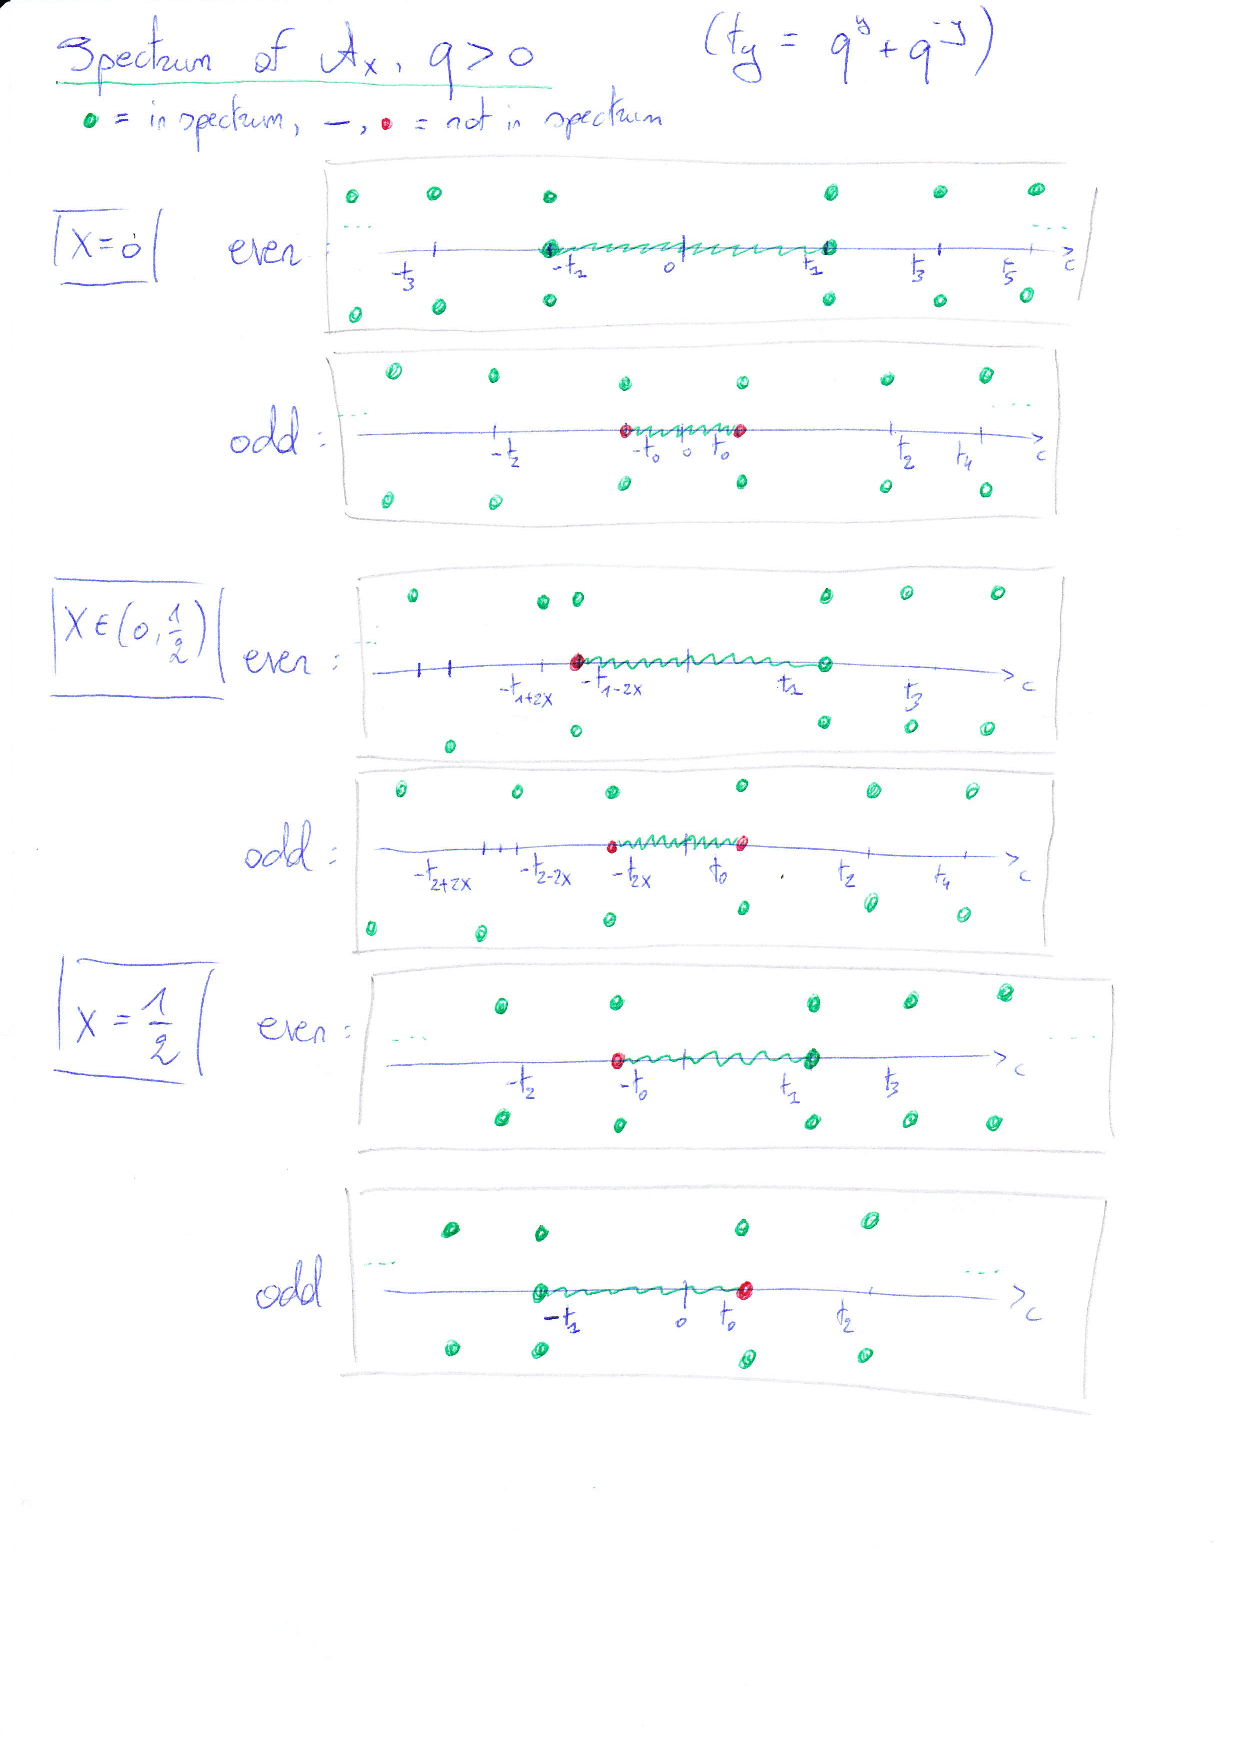
\includepdf[pages={1}]{ScanSpec.pdf}


% Make remark on regular representation cf. Koelink-Rosengren

% Include a concrete descripition of the universal envelope of $A_x$ from this?


%More generally, 

%As a concrete instance of the example of monoidal equivalence, let $\tilde{A}$ be the generalized compact Hopf face algebra obtained from the set $\tilde{I} =I_1\sqcup I_2$ with $I_1= \Z$ and $I_2= \{\bullet\}$ with the $B_{kl} =\emptyset$ and $E(k,l)$ for $k,l\neq \bullet$ as in section ..., with $B_{k,\bullet} = B_{\bullet,k}= \emptyset$, and $B_{\bullet,\bullet} = \{\pm\}$ with $E_{\bullet,\bullet} = \begin{pmatrix} 0 & |q|^{1/2} \\ -\sgn(q)|q|^{-1/2}&0\end{pmatrix}$ (with the basis ordered as $-,+$). Then this will be obtained from the direct sum of the functor from ... and the ordinary forgetful functor from $\Rep(SU_q(2))$ into $\Hilb$. It follows that the components $\tilde{A}(ij)$ can be described by the generators and relations as in ..., but with $F(\lambda)$ and $F(\rho)$ set equal to 1 whenever the corresponding index is $\bullet$.




% Study spectrum fundamental character
% Study dual quantum groupoid
% Make connection with dynamical cocycle
% In case of qgroupoid constructed from identity functor for Rep(SU_q(2)): rep theory of associated Galois object should just be: a single representation (Galois object is type I factor, cutdown of $B(\mathscr{L}^2(SU_q(2)))$). Yes: in general, Galois object is Morita equivalent with algebra of original ergodic action, should also be stressed for Podles spheres

\subsection{The reduced C$^*$-algebra of the dynamical quantum $SU(2)$ group}



% Notation $\weps$ should be recalled?
In \cite{KoR1}, the corepresentation theory of the dynamical quantum $SU(2)$ group is investigated. Transporting their definition to our setting, let us say an \emph{$n$-dimensional KR-corepresentation} consists of $n^2$ elements $t_{kl} \in M(A_x)$, together with an assigment $k \mapsto q_k \in q^{\Z}$ such that \begin{align*} \Delta(t_{km}) = \Delta(1)\left(\sum_{l=1}^n t_{kl}\otimes t_{lm}\right)&& \weps(t_{kl})\delta_y = \delta_{kl} \delta_{q_ky},&& f(\lambda,\rho)t_{kl} = t_{kl}f(q_k\lambda,q_l\rho),\end{align*} where $\widetilde{\epsilon}$ was introduced in \eqref{eq:weps}. Moreover, a KR-corepresentation is called \emph{unitary} if $S(t_{ij})^* =t_{ji}$, with $S$ the antipode of $SU_{q,x}^{\dyn}(2)$. For example, we see that the generating matrix $(u_{\epsilon,\nu})$ is a unitary 2-dimensional KR-corepresentation.  

To relate this to the corepresentations of Definition \ref{DefUniCorep}, put \[\left(\Gr{t}{y}{z}{v}{w}\right)_{kl} = \delta_{y}(\lambda)\delta_v(\rho) t_{kl} \delta_{z}(\lambda)\delta_{w}(\rho).\] Then this defines a unitary corepresentation on the collection of Hilbert spaces $V_{y,z}$ where $V_{y,z}=\{0\}$ except when there exists $k$ with $y = q_kz$,  in which case $V_{y,z} = \mathbb{C}^n$ (and with the matrix coefficients with respect to the canonical basis). 

According to \cite{KoR1}, there is a unitary $2N+1$-dimensional KR-corepresentation $t^N$ for each half-integer $N$ (dropping the tilde appearing in \cite{KoR1}), and moreover the fusion rules of the $t^N$ are the same as for $SU(2)$. On the other hand, we know from \cite[Section 5]{DCT1} that the tensor category of unitary representations of $SU_{q,x}^{\dyn}(2)$ is the same as the one for $SU_q(2)$, so we can also find a natural family of mutually non-equivalent irreducible unitary corepresentations $\mathscr{X}^{N}$ labelled by half-integers $N$. As the tensor products of corepresentations in the sense of \cite{KoR1} and \cite{DCT1} are compatible, we can thus deduce that the unitary corepresentations associated to the unitary KR-corepresentations $t^N$ also form a maximal family of non-equivalent irreducible unitary corepresentations. By using the concrete identification of \eqref{EqKR}, we have in particular that $t^{1/2}$ coincides with $(u_{\epsilon,\nu})_{\epsilon,\nu}$. 

  %Moreover, we can label the bases of our vector spaces by integers or halfintegers in such a way that $f(\lambda,\rho)t_{kl}^N = t_{kl}^Nf(q^{-k}\lambda,q^{-l}\rho)$. 

%From the general theory of \cite{DCT1}, we infer that the $\delta_y(\lambda)\delta_z(\rho)t_{kl}^N$ form an orthogonal (but not necessarily orthonormal) basis of $L^2(SU_q(2)_{\dyn})$. 

It then follows straightforwardly from \cite[Section 7]{KoR1} that, with $\varphi_{y,z}$ denoting the invariant integral on $\Gr{(A_x)}{y}{y}{z}{z}$ and $p$ any polynomial,  \[\varphi_{y,z}(p(\Omega)) = \int_{\R} p(s)\rd m_{y,z}(s),\] where $m_{y,z}$ is the normalized orthogonality measure for the (rescaled) Askey-Wilson polynomials \[p_k(s) = p_k(2s;qz/y,qy/z,-qyz,-q/yz;q^2).\]  From \cite[Theorem 2.1 and Theorem 2.5]{AsW1}%see also Koelink-Verding
, it follows that the support of $m_{y,z}$ is the union of the interval $\lbrack -2,2\rbrack$ with the set \[D_{y,z} = \{\tau(eq^k)\mid e\in \{qz/y,qy/z,-qyz,-q/yz\}, k\geq 0, |eq^k|>1\}.\]

In particular, we deduce the following corollary. Let us write $\mathcal{A}_x^r$ for the reduced C$^*$-algebra of $SU_{q,x}^{\dyn}(2)$.

\begin{Cor} The spectrum of $\Omega \,\eta\, \mathcal{A}_x^r$ equals $\lbrack -2,2\rbrack \cup \tau(q^{\Z}) \cup \tau(-x^2q^{\Z})$.
\end{Cor} 

In particular, as this spectrum is strictly smaller than the spectrum of $\Omega$ in $\mathcal{A}_x^u$ in Corollary \ref{CorSpecUni}, we obtain the following theorem.

\begin{Theorem} The partial compact quantum group $SU_{q,x}^{\dyn}(2)$ is not coamenable.
\end{Theorem} 




%%% Local Variables: 
%%% mode: latex
%%% TeX-master: "dynamical-SUq-file"
%%% End: 

%\section{The C$^*$-algebras of the canonical partical compact quantum group $\mathscr{G}(\Rep(SU_{\sigma q}(2))$}\label{SecUni}

In this final section, we look at the canonical partial compact quantum group associated to the Temperley-Lieb C$^*$-tensor category $\Rep(SU_{\sigma q}(2))$, and show that it is coamenable.

\subsection{Definition}

Denote $\tau_{\pm}(y) = y\pm y^{-1}$. Fix also $q>0$ and $\sigma\in \{\pm\}$. Consider the following $-\sigma(q+q^{-1})$-reciprocal random walk $\Gamma_{\can}$ \cite[Definition 5.1]{DCT1}: the underlying graph has vertices $q^{\N_0}$ and edge set $\{(y,z)\mid y/z \in \{q^{\pm 1}\}\}$, and we give them the weights $w(y,z) = \frac{\tau_-(z)}{\tau_-(y)}$ and signs $\sgn(y,qy) = +, \sgn(y,y/q) = -\sigma$. The involution is given by $\overline{(y,z)} = (z,y)$. This is the reciprocal random walk associated to $\Rep(SU_{\sigma q}(2))$ considered as a module category over itself, see the discussion following \cite[Definition 5.1]{DCT1}.

By that same discussion, we have an associated non-trivial partial compact quantum group $\mathscr{G}_{\can}$ with the same representation tensor C$^*$-category as $SU_{\sigma q}(2)$. By \cite[Theorem 5.2]{DCT1}, its associated partial Hopf $^*$-algebra $A =A_{\can}$ is generated by two copies of the finite support functions on $q^{\N_0}$ as well as elements $u_{e,f} \in \Gr{A}{s(e)}{t(e)}{s(f)}{t(f)}$ for each couple of edges $e,f$, with relations \begin{align*} &u_{e,f}^* = \frac{\sgn(f)\sqrt{w(f)}}{\sgn(e)\sqrt{w(e)}}u_{\bar{e},\bar{f}},\end{align*} \begin{align*}
 &\sum_{t(g) = w} u_{g,e}^* u_{g,f} = \delta_{e,f} \UnitC{w}{t(e)}, &&\sum_{s(g) = v} u_{e,g}u_{f,g}^* = \delta_{e,f} \UnitC{s(e)}{v}.\end{align*} 

As the graph underlying the above reciprocal random walk is not homogeneous, we can not find as nice a subalgebra inside $M(A)$ as in the previous section. However, there is still a suitable analogue available. Namely, for $\epsilon,\nu \in \{-,+\}$, define inside $M(A)$ the elements \[u_{\epsilon,\nu} =\underset{q^{\epsilon}y,q^{\nu}z \in q^{\N_0}}{ \sum_{y,z\in q^{\N_0}}} u_{(y,q^{\epsilon}y),(z,q^{\nu}z)}.\] Then we have the grading relation  $f(\lambda,\rho) u_{\epsilon,\nu} = u_{\epsilon,\nu}f(q^{-\epsilon}\lambda,q^{-\nu}\rho)$, where the value of a function is defined to be zero if its input is outside its domain of definition, together with \begin{align*}
& u_{\epsilon,\nu}^* \left(\tau_-(q^{\epsilon}\lambda)/\tau_-(\lambda)\right)^{1/2} = \sgn(\epsilon)\sgn(\nu) u_{-\epsilon,-\nu}\left(\tau_-(q^{\nu}\rho)/\tau_-(\rho)\right)^{1/2},\end{align*} 
\begin{align*} 
&\sum_{\mu} u_{\mu,\epsilon}^* u_{\mu,\nu} = \delta_{\epsilon,\nu}(1- \delta_{\epsilon,+}\delta_{q}(\rho)), && \sum_{\mu} u_{\epsilon,\mu}u_{\nu,\mu}^* = \delta_{\epsilon,\nu}(1-\delta_{\epsilon,-}\delta_{q}(\lambda)).\end{align*}

Let us denote as before $u_{-,-}=\alpha$ etc. Then the defining relations become 

\begin{equation*} \left\{\begin{array}{llllllll} \alpha \alpha^* +\beta\beta^* &=& 1-\delta_q(\lambda) && \gamma \gamma^* + \delta\delta^* &=& 1,\\
\alpha^*\alpha + \gamma^* \gamma &=& 1, && \beta^* \beta +\delta^*\delta &=&1-\delta_q(\rho),\\ \\  \alpha \gamma^* = -\beta \delta^*, &&&& \alpha^* \beta = -\gamma^* \delta,\end{array}\right.\end{equation*} 
and, writing $w_{\pm}(y) = \tau_-(q^{\pm 1}y)/\tau_-(y)$, 
\begin{align*} &\delta^* = \alpha \frac{w_-^{1/2}(q\lambda)}{w_-^{1/2}(q\rho)}, &&\gamma^* = -\sigma w_+^{-1/2}(\rho)\beta w_-^{1/2}(q\lambda),\\ 
&\beta^* = -\sigma w_-^{-1/2}(q\lambda)\gamma w_+^{1/2}(\rho),&&\alpha^* =  \frac{w_-^{1/2}(q\rho)}{w_-^{1/2}(q\lambda)}\delta.\end{align*}

Commutation relations between the generators and $\lambda,\rho$ are as before.

\subsection{Representation theory}

As before, we can construct a central element inside $M(A)$.

\begin{Lem} The element $\Omega = \tau_+(\lambda/q\rho)+\tau_-(\lambda)\tau_-(q\rho)\gamma^*\gamma$ is a central and selfadjoint element in $M(A)$.
\end{Lem}
\begin{proof} Elementary.
\end{proof}

Also the following lemma is as straightforward as before.

\begin{Lem}\label{LemOm}  \begin{align*}  & \alpha^*\alpha = \frac{\tau_+(q\lambda\rho)-\Omega}{\tau_-(\lambda)\tau_-(q\rho)}, && \gamma^*\gamma = \frac{\Omega - \tau_+(\lambda/q\rho)}{\tau_-(\lambda)\tau_-(q\rho)} 
\end{align*}
%\\ &\gamma \gamma^* = \frac{\Omega- \tau_+(q\lambda/\rho)}{\tau_-(q\lambda)\tau_-(\rho)} \\ &\delta \delta^* = \frac{\tau_+(q\lambda\rho)-\Omega}{\tau_-(q\lambda)\tau_-(\rho)} \\ & \delta^*\delta \tau_-(\rho/q)\tau_-(\lambda) = \tau_+(\lambda\rho/q)-\Omega.
\end{Lem} 

\begin{Lem} For each $m\in \N_0$, there exists exactly one irreducible representation $\pi_m$ of $A$ with $\pi_m(\Omega) = \tau_+(q^m) = q^m+q^{-m}$, and this exhausts all irreducible representations. Moreover, a concrete realization of $\pi_m$ is on the Hilbert space $\mathscr{H}_m = l^2(W_{m})$ with $W_m$ the `well' \[W_m = \{(q^k,q^l)\mid k,l\in \N_0, |k-l\pm1|\leq m \leq k+l-1\}\] and where the representation is determined by \begin{align*} & \lambda e_{y,z} = ye_{y,z},&& \rho e_{y,z} = z e_{y,z},\\
&\alpha e_{y,z} = \left(\frac{\tau_+(qyz)-\tau_+(q^m)}{\tau_-(y)\tau_-(qz)}\right)^{1/2} e_{qy,qz}, &&\beta e_{y,z} = \sigma_y \left(\frac{\tau_+(q^m)-\tau_+(qy/z)}{\tau_-(y)\tau_-(z/q)}\right)^{1/2}e_{qy,z/q}, \\
&\gamma e_{y,z} = -\sigma_y \left(\frac{\tau_+(q^m)-\tau_+(y/qz)}{\tau_-(y)\tau_-(qz)}\right)^{1/2} e_{y/q,qz}, && \delta e_{y,z} = \left(\frac{\tau_+(yz/q)-\tau_+(q^m)}{\tau_-(y)\tau_-(z/q)}\right)^{1/2} e_{y/q,z/q},\end{align*}
where $e_{y,z}$ is interpreted as the zero vector when $(y,z)\notin W_m$. 
\end{Lem} 

\begin{proof}% Elegant proof of first assertion? 
It can be proven in a straightforward (but slightly tedious) way that the set of elements \[\{\delta_{y}(\lambda)\delta_{z}(\rho)\alpha^m\beta^n\gamma^k\delta^l\mid k,l,m,n\in \N,y,z\in q^{\N_0}\}\] spans $A$. It follows that if $(\Hsp,\pi)$ is any non-degenerate irreducible representation of $A$, then the $\Hsp^y_z$ are at most one-dimensional for each $y,z\in q^{\N_0}$. 

Fix $(\Hsp,\pi)$, and write again $H = \oplus_{y,z\in q^{\N_0}} \Hsp^y_z$ for the algebraic direct sum of all $\Hsp^y_z$. It follows as before that the generators $\alpha,\beta,\gamma,\delta$ act as adjointable endomorphisms on $H$, and that $\Omega$ then acts as a scalar $c$. Write $T_{\pi} =\{(y,z)\mid \Hsp^{y,z}\neq \{0\}, y,z\in q^{\N_0}\}$. We can hence pick unit vectors $e_{y,z}\in \Hsp^y_z$ on which $A$ acts as in the statement of the lemma with $W_m$ replaced by $T_{\pi}$ and $q^m$ replaced by $c$.

Choose now $(y,z)\in T_{\pi}$ with $(y/q,qz)\notin T_{\pi}$. Then $\gamma^*\gamma e_{y,z} = 0$, hence $c=\tau_+(y/qz)$. So $c= \tau_+(q^m)$ for some $m\in \N$.

Let us first show that the kernel of $\alpha$ is zero. Suppose not, then there exists $(y,z)\in T_{\pi}$ with $\alpha e_{y,z}=0$. This implies $y= q^k$ and $z=q^l$ with $k,l\in \N_0$ and $k+l+1 = m$. In particular, $m\geq 2$. It follows from the well-definedness of the square root in the formula for $\delta$ that then necessarily $y=q$ or $z=q$, and in particular $e_{y,z}$ also in the kernel of $\delta$. It follows from irreducibility and the commutation relations between $\{\alpha,\delta\}$ and $\{\gamma,\beta\}$ that $\pi(\alpha) = \pi(\delta)=0$. But it is easy to check that dividing out by these relations forces also $\pi(\beta)=\pi(\gamma)=0$, giving a contradiction. 

As the kernel of $\alpha$ is zero, it follows that $(y,z)\in T_{\pi}$ implies $(qy,qz)\in T_{\pi}$. Denote now by $S_{\pi}$ the set of all $s\in \Z$ with $\{(y,q^sy)\mid y\in q^{\N_0}\}\cap T_{\pi}\neq \emptyset$. Then for each $s\in S_{\pi}$, we can find a unique element $(y_s,q^sy_s) \in T_{\pi}$ such that all $(y,z)\in T_{\pi}$ with $z/y= q^s$ are of the form $(q^ny_s,q^{n+s}y_s)$ for $n\in \N$, with all such elements appearing inside $T_{\pi}$. Looking at the actions of $\gamma$ and $\beta$, we see that if $s\in S_{\pi}$, then necessarily $-m+1\leq s\leq m-1$, enforcing $m\geq 1$. On the other hand, if $(q^k,q^l)\in T_{\pi}$, we see from the action of $\delta$ that necessarily $k+l-1\geq m$. 

It follows that $T_{\pi} \subseteq W_m$. To conclude the proof, it suffices to show that the proposed action on $l^2(W_m)$ is well-defined and irreducible. Well-definedness is immediate. Irreducibility follows also straightforwardly.
\end{proof}


\subsection{Coamenability}

In this section, we prove that $\mathscr{G}_{\can}$ is coamenable. For this, we consider the auxiliary partial compact quantum group $\widetilde{\mathscr{G}}_{\can}$, obtained by enlarging our previous graph $\Gamma_{\can}$ `at infinity' with the vertex $0$ and two edges $e_{\pm}$ from 0 to itself with weights $q^{\mp 1}$ and signs $\sgn(e_+)=+,\sgn(e_-)=-\sigma$. The resulting algebra $\widetilde{A}$ will then split into a direct sum of four $^*$-algebras \[\widetilde{A} = A_{\can,\can} \oplus A_{\can,\bullet} \oplus A_{\bullet,\can} \oplus A_{\bullet,\bullet},\] where for example $A_{\can,\bullet} = \delta_{q^{\N_0}}(\lambda)\delta_0(\rho) \widetilde{A}$. From the discussion in \cite[Section 4.2]{DCT1}, it follows that $A_{\can,\can}$ is the $^*$-algebra $A_{\can}$ from before, whereas $A_{\bullet,\bullet}$ will be the $^*$-algebra associated to the compact quantum group $SU_q(2)$. The same discussion also provides us with homomorphisms \[\Delta_{a,b}^c: A_{ab}\rightarrow M(A_{ac}\otimes A_{cb}),\qquad a,b,c \in \{\bullet,\can\},\] which allows us to take tensor representations of $A_{ac}$ and $A_{cb}$ to a representation of $A_{ab}$.

Note that the Haar functional on $\widetilde{A}$ restricts to a faithful functional on each of the components, so it makes sense to talk of the regular representation. Moreover, the restriction of the Haar functional to $A_{\can,\can}$ gives precisely the Haar functional on $A_{\can}$.

\begin{Lem} Let $\pi_{\reg}^{a,b}$ be the regular representation of $A_{a,b}$ for $a,b\in \{\can,\bullet\}$. Then $\pi_{\reg}^{\can,\can} \preceq \pi_{\reg}^{\can,\bullet}\boxtimes \pi_{\reg}^{\bullet,\can}$. 
\end{Lem} 

\begin{proof} Let $\phi$ be the Haar functional on $\widetilde{A}$, and denote by $\phi_{km}$ its restriction to $\gr{\widetilde{A}}{k}{k}{m}{m}$. Then by definition of invariance, we find by invariance of $\phi$ (and the fact that $\UnitC{k}{\bullet}\neq 0$ for all $k$) that for all $a\in A_{\can,\can}$, \[(\phi\otimes \phi)\Delta_{\bullet,\bullet}(a) = \phi(a).\] This implies the lemma.
\end{proof}


Hence, we want to study the representation theory of $A_{\can,\bullet}$ and its companion $A_{\bullet,\can}$. Note that inside $M(A_{\can,\bullet})$ we can define `generators' $\alpha,\beta,\gamma,\delta$ just as before, by putting all occurences of $\rho$ in the defining relations equal to $0$. 

\begin{Lem} Up to equivalence, there is only one irreducible $^*$-representation $\pi_L$ of $A_{\can,\bullet}$. A concrete realization of it is given on $l^2(W_{L})$ with \[W_L= \{(q^k,q^l)\mid k\in \N_0,l\in \Z, \{k-l,k+l\}\subseteq 2\N+1\}\] by the formulas \begin{align*}& \lambda e_{y,z} =ye_{y,z},\\
 &\alpha e_{y,z}  = \left(\frac{qz-1/y}{\tau_-(y)}\right)^{1/2} e_{qy,qz}, && \beta e_{y,z}= \sigma_y \left(\frac{y-z/q}{\tau_-(y)}\right)^{1/2} e_{qy,z/q}\\ &\gamma e_{y,z} = -\sigma_y \left(\frac{y-qz}{\tau_-(y)}\right)^{1/2}e_{y/q,qz} &&\delta e_{y,z} = \left(\frac{z/q-1/y}{\tau_-(y)}\right)^{1/2} e_{y/q,z/q},\\ 
\end{align*}
\end{Lem}

\begin{proof} Consider the element $\Omega_{\rho} = \lambda/q+q^{-1}\tau_-(\lambda)\gamma^*\gamma$, which is a formal limit $\lim_{\rho\rightarrow 0} \rho\Omega$ with $\Omega$ in $A_{\can}$ as before. Then it follows that $\Omega_{\rho}$ $q$-commutes with the generators $\alpha,\beta,\gamma,\delta$. 

Let $\pi$ be an irreducible representation of $A_{\can,\bullet}$. It is easy to see that, by irreducibility and $q$-commutation rules, the spectrum of $\Omega_{\rho}$ is purely discrete. Moreover, by the precise formula of $\Omega_{\rho}$, it follows that the spectrum is strictly positive. It then follows as before, using the limit analogues of the identities in Lemma \ref{LemOm}, that if $S_{\pi}$ is the spectrum of $\Omega_{\rho}$, each $\Hsp^y_z$ with $y\in q^{\N_0}$ and $z\in \Spec(\Omega_{\rho})$ is at most one-dimensional, and that, denoting $T_{\pi}$ for the set of $(y,z)\in q^{\N_0}\times S_{\pi}$ with $\Hsp^y_z\neq \{0\}$, we can find unit vectors $e_{y,z}$ for $(y,z)\in T_{\pi}$ such that the representation acts as in the statement of the lemma.  

Now choose $(y,z)\in T_{\pi}$ with $(y/q,qz)\notin T_{\pi}$. Then we deduce from the action of $\gamma$ that $y=qz$, and in particular $S_{\pi} \subseteq q^{\Z}$. But it is also clear that $e_{y,y/q}$ is not in the kernel of $\delta$ for $y\neq q$. It follows that $(q,1) \in T_{\pi}$. Moreover, as $\gamma e_{q,1} = \delta e_{q,1}$, it follows that $T_{\pi}\subseteq W_L$. As before, it then suffices to check that the given action on $l^2(W_L)$ is well-defined and irreducible.

\end{proof}

It follows in particular that the regular representation of $A_{\can,\bullet}$ is just a multiple of the above representation.

Using the unitary antipode of $\widetilde{A}$, we can find a $^*$-isomorphism $\theta:A_{\bullet,\can}\rightarrow A_{\can,\bullet}$ by \begin{align*} &\alpha \mapsto q^{-1/2}w_-^{1/2}(\lambda)\alpha,&&\beta \mapsto -\sigma \beta^* &&\rho\mapsto \lambda\end{align*} 

As a result, we obtain the next corollary. 

\begin{Cor} Up to equivalence, there is only irreducible $^*$-representation $\pi_R$ of $A_{\bullet,\can}$. A concrete realization of it is given on $l^2(W_R)$ with \[W_R= \{(q^k,q^l)\mid k\in \Z,l\in \N_0, \{l-k,k+l\}\subseteq 2\N+1\}\] by the formulas \begin{align*} & \rho e_{y,z} =z e_{y,z} \\ &\alpha e_{y,z}  = \left(\frac{y-1/qz}{\tau_-(qz)}\right)^{1/2} e_{qy,qz},&& \beta e_{y,z}= -\sigma_z \left(\frac{z/q-y}{\tau_-(z/q)}\right)^{1/2} e_{qy,z/q},\\ &\gamma e_{y,z} = \sigma_z \left(\frac{qz-y}{\tau_-(qz)}\right)^{1/2}e_{y/q,qz},  &&\delta e_{y,z} = \left(\frac{y-q/z}{\tau_-(z/q)}\right)^{1/2} e_{y/q,z/q}.\\ 
\end{align*}
\end{Cor}

\begin{Theorem} The partial compact quantum group $\mathscr{G}_{\can}$ is coamenable.
\end{Theorem}
\begin{proof} It suffices to check that the trivial representation of $\mathscr{G}_{\can}$ is weakly contained in $\pi = \pi_L\boxtimes \pi_R$. Now the latter is a (non-degenerate) representation on $l^2(W_L)\otimes l^2(W_L)$, and a small calculation yields \begin{align*} &\hspace{-0.4cm}\pi(\Omega)e_{y,z,y',z'} \\ &= -\sigma_y\sigma_{z'} \left[(1-yz/q)(1-z/qy)(1-y'/qz')(1-y'z'/q)\right]^{1/2} e_{y,z/q^2,y'/q^2,z'} \\ &+ \left[\tau_+(y/qz') -\frac{qz'}{y}(1-yz/q)(1-y'/qz') -\frac{y}{qz'}(1-qz/y)(1-qy'z')\right] e_{y,z,y',z'} \\ & - \sigma_y\sigma_z'\left[(1-qyz)(1-qz/y)(1-qy'/z')(1-qy'z')\right]^{1/2} e_{y,q^2z,q^2y',z'}.\end{align*} 

It follows immediately that $e_{q,1,1,q}$ is an eigenvector of $\pi(\Omega)$ at eigenvalue $q+q^{-1}$, hence the representation spanned by $e_{q,1,1,q}$ is nothing but the trivial representation itself. 
\end{proof} 







%%% Local Variables: 
%%% mode: latex
%%% TeX-master: "dyn-suq-main"
%%% End: 

\bibliographystyle{abbrv}
\bibliography{referencesSUq}
% \begin{thebibliography}{99}
% \bibitem{AN1} N. Andruskiewitsch and S. Natale, Double categories and quantum groupoids, \emph{Publ. Mat. Urug.} \textbf{10}, 11--51 (2005).
% \bibitem{BDV1} J. Bichon, A. De Rijdt and S. Vaes, Ergodic coactions with large multiplicity and monoidal equivalence of quantum groups, \emph{Comm. Math. Phys.} \textbf{262} (2006), 703--728.
% \bibitem{Boh1}  G. B\"{o}hm, J. Gómez-Torrecillas and E. López-Centella, Weak multiplier bialgebras, \emph{Trans. Amer. Math. Soc.}, in press., arXiv:1306.1466. 
% \bibitem{Dau1} J. Dauns, Multiplier rings and primitive ideals, \emph{Trans. Amer. Math. Soc} \textbf{145} (1969), 124--158.
% \bibitem{DCY1} K. De Commer and M. Yamashita, Tannaka-Kre\u{\i}n duality for compact quantum homogeneous spaces II. Classification of quantum homogeneous spaces for quantum $SU(2)$, J. Reine Angew. Math., DOI: 10.1515/crelle-2013-0074 (2013).
% \bibitem{Eti1} P. Etingof and V. Ostrik, Module categories over representations of $\SSL_q(2)$ and graphs, \emph{Math. Res. Lett.} \textbf{11} (1) (2004), 103--114.
% \bibitem{Hay1} T. Hayashi, Compact Quantum Groups of Face Type, \emph{PRIMS} \textbf{32} (1996), 351--369.
% \bibitem{KoR1}  E. Koelink and H. Rosengren, Harmonic Analysis on the $SU(2)$ Dynamical Quantum Group, \emph{Acta Applicandae Mathematica} \textbf{69} (2) (2001), 163--220.
% \bibitem{Pin2} C. Pinzari, The representation category of the Woronowicz quantum group $S_{\mu}U(d)$ as a braided tensor C$^*$-category, \emph{Int. J. Math.} \textbf{18} (2) (2007), 113--136.
% \bibitem{Pin3} C. Pinzari and J.E. Roberts, Ergodic actions of compact quantum groups from solutions of the conjugate equations, preprint (2008) {\tt arXiv:0808.3326 [math.OA]}.
% \bibitem{Tur1} V. Turaev, Quantum invariants of knots and 3-manifolds, \emph{de Gruyter Studies in Mathematics} \textbf{18}, Walter de Gruyter \& Co., Berlin (1994).
% \bibitem{VDae1} A. Van Daele, Multiplier Hopf algebras, \emph{Trans. Amer. Math. Soc.} \textbf{342} (1994), 917--932.
% \bibitem{VDae2} A. Van Daele, An algebraic framework for group duality, \emph{Adv. in Math.} \textbf{140} (1998), 323--366.
% \bibitem{VDW2} A. Van Daele and  S. Wang, Weak multiplier Hopf algebras. Preliminaries, motivation and basic examples, \emph{Banach Center Publ.} \textbf{98} (2012), 367--415.
% \bibitem{VDW1} A. Van Daele and S. Wang: Weak multiplier Hopf algebras I. The main theory, \emph{Preprint University of Leuven and Southeast University of Nanjing} (2012), to appear in
% \emph{Crelles Journal}, {\tt arXiv:math/1210.4395 [math.RA]}.
% \bibitem{Yam1} S. Yamagami, A categorical and diagrammatical approach to Temperley--Lieb algebras, preprint (2004) {\tt arXiv:math/0405267 [math.QA]}.
% \bibitem{Wor1} S.L. Woronowicz, Twisted $\mathrm{SU}(2)$ group. An example of a non-commutative differential calculus, \emph{Publ. Res. Inst. Math. Sci.} \textbf{23} (1) (1987), 117--181.
% \end{thebibliography}

\end{document}
